% !TEX TS-program = lualatexmk

\documentclass[10pt, a4paper]{scrbook}
% !TEX root = ../main.tex
\KOMAoptions{
    headings=standardclasses,
    bibliography=totoc,
    toc=indentunnumbered,
    usegeometry
}

%%% FIX
\let\ifstr\Ifstr

%%% GEO
% \usepackage[bottom=3.5cm, inner=2.5cm,outer=3.5cm, marginpar=3.5cm, includeheadfoot]{geometry} % NEL CASO b5paper
\usepackage[bottom=3.5cm, inner=3.5cm,outer=4.5cm, marginpar=3.5cm, includeheadfoot]{geometry} % NEL CASO a4paper

%% Pagestcyle
\usepackage[automark]{scrlayer-scrpage}
\pagestyle{scrheadings}
\lehead{\thepage \qquad \leftmark}
\rohead{\rightmark \qquad \thepage}
\ofoot{}

%%% LANGUAGE AND FONT
\usepackage[english]{babel}
\usepackage[utf8]{inputenc}
\usepackage[T1]{fontenc}

% \usepackage[babel=true]{microtype}
\usepackage{helvet}
\usepackage{mathpazo}
% \usepackage{vicent}


\usepackage{amsmath,amssymb,amsfonts}
\usepackage[makeroom]{cancel}
\usepackage{siunitx}
\usepackage{physics}
% SIUNITX
\sisetup{
    per-mode=symbol,
    separate-uncertainty=true,
    range-units=single,
    range-phrase=\text{\ to\ }
}
\DeclareSIPrefix\micro{\text{\textmu}}{-3}

\usepackage[numbers, sort&compress]{natbib}
\usepackage[american, useregional]{datetime2}

\usepackage[pagebackref=true]{hyperref}
% Hyperref setup, hidelinks in definition.
\hypersetup{
    pdfauthor={M Sotgia <mattia.sotgia@ge.infn.it>},
    pdfcreator={Latex/UNIGE (\DTMnow)},
    pdftitle={Opening Pandora's box},
    pdfsubject={A dedicated study of the automatic event reconstruction in the ICARUS experiment}
}
\usepackage{lastpage}
\usepackage[figure,table]{totalcount}

\usepackage[dvipsnames]{xcolor}

\usepackage{graphicx}
\graphicspath{{6_figures/}}
\usepackage{marginnote}
\usepackage[some]{background}
\usepackage{subfig}
\usepackage{sidecap}
\usepackage{booktabs}
\usepackage{longtable}
\usepackage{multirow}

\usepackage{paralist}

\usepackage{rotating}

\usepackage{tikz}
\usepackage{pgfplots}
\usepackage{tikz-feynman}
% Tikz libraries
\usetikzlibrary{
    angles, 
    arrows, 
    arrows.meta, 
    backgrounds,
    calc, 
    decorations.pathmorphing, 
    intersections, 
    positioning, 
    quotes, 
    shapes, 
    shapes.geometric,
    spath3
}
\pgfplotsset{compat=1.18}


% Table of contents style
\RedeclareSectionCommands[%
  toclinefill={,\qquad},%
  tocraggedpagenumber,%
  tocpagenumberbox=\mbox,
]{part,chapter,section, subsection, subsubsection}

\RedeclareSectionCommands[%
    tocdynindent,
    tocindentfollows=chapter
]{section}

\RedeclareSectionCommands[%
    tocdynindent,
    tocindentfollows=section
]{subsection}

\RedeclareSectionCommands[%
    tocdynindent,
    tocindentfollows=subsection
]{subsubsection}

\addtokomafont{chapterentry}{\mdseries}
\DeclareTOCStyleEntry[
  entrynumberformat=\bfseries\sffamily,
  dynnumwidth
]{chapter}{chapter}
\let\oldaddchaptertocentry\addchaptertocentry
\renewcommand{\addchaptertocentry}[2]{%
    \ifstr{#1}{}{%
        \oldaddchaptertocentry{#1}{#2}}{%
        \oldaddchaptertocentry{\chapapp{} #1}{#2}%
}}


% update \appendix definition
\let\oldappendix\appendix
\renewcommand{\appendix}{
\oldappendix
\counterwithin{equation}{chapter}
\counterwithin{figure}{chapter}
\counterwithin{table}{chapter}
}

% Figures and tables style
\setcapindent{0pt}
\addtokomafont{captionlabel}{\bfseries}
\renewcommand*{\captionformat}{\ }



% Chapter style
% \renewcommand{\thechapter}{\Roman{chapter}}
% \renewcommand{\thesection}{\normalfont \arabic{section}} % Workaraund
% \addtokomafont{subsection}{\normalfont\itshape}
% \addtokomafont{chapter}{\MakeUppercase}

% Marginnotes
% \renewcommand{\marginfont}{\sffamily\small}
% \newcommand{\note}[1]{\marginnote{
% \colorbox{yellow}{\begin{minipage}{\marginparwidth}
% #1
% \end{minipage}}
% }}

% \usepackage{showframe}

% Background WM
\backgroundsetup{
    % position={-1.5cm,-16cm},
    position={-1.5cm,-13cm},
    color=black, opacity=1, scale=1,
    angle=90
}
\SetBgContents{
    % \hspace{0.1cm}
    \begin{minipage}[b]{8cm}
        \fontfamily{ptm}\selectfont
        UNIGE / FNAL / THESIS-\the\year-\the\month\ % \\
        % \DTMNow\
        (\pageref{LastPage} pp, \totalfigures\ figs.)
    \end{minipage}
\includegraphics[height=1cm]{6_figures/FNAL/FNAL-Logo-Black}
}

% bibliography pageref

\renewcommand*{\backref}[1]{}
\renewcommand*{\backrefalt}[4]{
    % \color{gray}
    \color{chaptergrey}
    \ifcase #1 (Not cited.)%
          \or{Cited on p. #2}%
          \else{Cited on pp. #2}%
    \fi%
}

\renewcommand\bibnumfmt[1]{#1.}
\urlstyle{sf}

% dictum redefinitions
% \setkomafont{dictum}{\normalfont}
\renewcommand*\dictumwidth{0.45\linewidth}

% Title and other strong commands definitions

\DeclareRobustCommand\title[1]{
\gdef\@title{#1}
}

% \usepackage[Lenny]{fncychap}
\usepackage[utopia]{quotchap}

\makeatletter 
\renewcommand*{\sectfont}{\bfseries}
\renewcommand*{\chapnumfont}{%
% \usefont{T1}{\@defaultcnfont}{b}{n}\fontsize{130}{160}\selectfont% Default: 100/130
% \cursiveshape
\usefont{T1}{phv}{bx}{n}%
\fontsize{100}{130}\selectfont% Default: 100/130
\color{chaptergrey}%
\phantom{0}% This fixes chapter w/o number
}
\makeatother
\addtokomafont{chapter}{\usefont{T1}{phv}{b}{n}\selectfont}
% \addtokomafont{section}{\sffamily}
% \addtokomafont{subsection}{\sffamily}
% \addtokomafont{subsubsection}{\sffamily}

\definecolor{chaptergrey}{rgb}{0.6862745098,0.1529411765,0.1843137255}
% \colorlet{chaptergrey}{PineGreen}
\colorlet{chaptergrey}{ForestGreen}
% \definecolor{chaptergrey}{rgb}{0.2980392157,0.5490196078,0.168627451} % 76, 140, 43
% \colorlet{chaptergrey}{NavyBlue}

\hypersetup{colorlinks, allcolors=chaptergrey}

\newenvironment{abstract}
    {%
    \cleardoublepage
    \phantom{.}\par%
    \vfill\par%
    \begin{center}
    {\bfseries Abstract}
    \end{center}
    }
    {%
    \par%
    \vfill\vfill\phantom{.}
    }

\usepackage{listings}
    
\definecolor{codegray}{gray}{0.9}
\definecolor{darkblue}{rgb}{0,0,0.6}
\definecolor{darkgreen}{rgb}{0,0.5,0}
\definecolor{darkred}{rgb}{0.6,0,0}

%% LISTINGS (ahaahha there ill be a lot :)
\lstdefinestyle{xmlstyle}{
    language=XML,
    % basicstyle=\small,
    columns=flexible,
    numbers=left,
    numberstyle=\tiny\color{gray},
    stepnumber=1,
    % numbersep=5pt,
    % backgroundcolor=\color{codegray},
    showspaces=false,
    showstringspaces=false,
    breaklines=true,
    frame=single,
    % frame=l,
    morekeywords={pandora, algorithm,InputCaloHitListName, ClusterListName, ReplaceCurrentCaloHitList, ReplaceCurrentClusterList, CollapseToPrimaryMCParticles, MCParticleListName},
    keywordstyle=\color{RoyalBlue},
    stringstyle=\color{Peach},
    commentstyle=\itshape\color{gray}
}

\renewcommand{\labelitemi}{$\textcolor{chaptergrey}{\circ}$}
\renewcommand{\labelitemii}{$\textcolor{chaptergrey}{\circ}$}
\renewcommand{\labelitemiii}{$\textcolor{chaptergrey}{\circ}$}
\renewcommand{\labelitemiv}{$\textcolor{chaptergrey}{\circ}$}

\renewcommand{\labelenumi}{\textcolor{chaptergrey}{\arabic{enumi}.}}
\renewcommand{\labelenumii}{\textcolor{chaptergrey}{\alph{enumii})}}
\renewcommand{\labelenumiii}{\textcolor{chaptergrey}{\roman{enumiii}.}}
\renewcommand{\labelenumiv}{\textcolor{chaptergrey}{\Alph{enumiv}.}}

\newif\ifdraft
\draftfalse


\usepackage{eso-pic}
\usepackage{duerer}

\renewcommand{\floatpagefraction}{.95}%


\usepackage{longtable}
\newenvironment{abbreviations}[1][.5em]{
\par\vspace{#1}\noindent\begin{longtable}{@{}>{\bfseries}p{0.25\linewidth}@{\hspace{0.025\linewidth}}p{0.725\linewidth}@{}}
}{
\end{longtable}
}

%%%---thumb indices using chapterthumb

% the following bases on an example in the KOMA-Script book:
\newcommand*{\firstchapterthumbskip}{.1\paperheight}
\newcommand*{\lastchapterthumbskip}{\firstchapterthumbskip}
\newcommand*{\chapterthumbheight}{.1\paperheight}
\newcommand*{\chapterthumbwidth}{.01\paperheight}
\newcommand*{\chapterthumbskip}{.1\paperheight}
\colorlet{chapterthumbboxcolor}{chaptergrey!75}
\newcommand*{\chapterthumbcolor}{white}
\newcommand*{\chapterthumbformat}{\thechapter}
\newkomafont{chapterthumb}{\normalfont\Large\color{\chapterthumbcolor}}

\makeatletter
\newcommand*\chapterthumb@box{%
    \usekomafont{chapterthumb}%
    \parbox[c][\chapterthumbheight][c]{\chapterthumbwidth}{%
        \centering
        \begin{tikzpicture}
        \node[minimum width=2.5cm, minimum height=2.5cm, fill=chapterthumbboxcolor] % chapterthumbboxcolor
        {\ifodd\value{page}\makebox[0pt][c]{\hspace{-1cm}\chapterthumbformat} \else\makebox[0pt][c]{\hspace{1cm}\chapterthumbformat}\fi};
        \end{tikzpicture}%
    }%
}
\newcommand*{\chapterthumbbox}{%
    \if@mainmatter
    \ifnum\value{chapter}>\z@
    \ifnum \value{chapterthumb}<\z@
    \else
    \begingroup
    \protected@edef\reserved@a{\chapterthumbformat}%
    \ifx\reserved@a\lastchapterthumbformat\else
    \stepcounter{chapterthumb}%
    \global\let\lastchapterthumbformat\reserved@a
    \fi
    \@tempcnta=\numexpr
    \dimexpr
    \paperheight
    -\firstchapterthumbskip
    -\chapterthumbwidth
    -\lastchapterthumbskip
    \relax / \dimexpr
    \chapterthumbskip
    \relax
    +1
    \relax
    \ifnum \value{chapterthumb}<\@tempcnta
    \else
    \setcounter{chapterthumb}{0}%
    \fi
    \vspace*{%
        \dimexpr
        \firstchapterthumbskip
        + ( \chapterthumbskip )
        * \value{chapterthumb}%
        - \baselineskip
        \relax
    }\par
    \setlength{\fboxsep}{0pt}%
    \ifodd\value{page}
    \hfill
    \makebox[0pt][r]{%
        \rotatebox[origin=c]{0}{\chapterthumb@box}}%
    \hspace*{1.5cm}
    \else
    \hspace*{-0.8cm}
    \makebox[0pt][l]{%
        \rotatebox[origin=c]{0}{\chapterthumb@box}}%
    \fi
    \endgroup
    \fi
    \fi
    \fi
}
\makeatother

\newcounter{chapterthumb}
\setcounter{chapterthumb}{10000}
\newcommand*{\lastchapterthumbformat}{\relax}

\DeclareNewLayer[%
background,%
outermargin,%
contents=\chapterthumbbox
]{chapterthumb}

\newcommand*\EnableChapterthumb{%
    \IfLayerAtPageStyle{scrheadings}{chapterthumb}{}
    {\AddLayersToPageStyle{@everystyle@}{chapterthumb}}%
}
\newcommand*\DisableChapterthumb{%
    \RemoveLayersFromPageStyle{@everystyle@}{chapterthumb}%
}

\EnableChapterthumb

\newcommand{\tikzxmark}{%
\tikz[scale=0.23] {
    \draw[Red, line width=0.7,line cap=round] (0,0) to [bend left=6] (1,1);
    \draw[Red, line width=0.7,line cap=round] (0.2,0.95) to [bend right=3] (0.8,0.05);
}}
\newcommand{\tikzsmark}{%
\tikz[scale=0.23] {
    \draw[Peach, line width=0.7,line cap=round] (0,0.1) to [bend left=6] (1,1);
    \draw[Peach, line width=0.7,line cap=round] (0.,0.65) to [bend left=4.5] (1.1,0.25);
    \draw[Peach, line width=0.7,line cap=round] (0.35,1.15) to [bend right=5] (0.6,0.0);
}}
\newcommand{\tikzcmark}{%
\tikz[scale=0.23] {
    \draw[Green, line width=0.7,line cap=round] (0.25,0) to [bend left=10] (1,1);
    \draw[Green, line width=0.8,line cap=round] (0,0.35) to [bend right=1] (0.23,0);
}}

\usepackage{mathtools}
\DeclarePairedDelimiter\ceil{\lceil}{\rceil}
\DeclarePairedDelimiter\floor{\lfloor}{\rfloor}

% !TEX root = ../main.tex
\def\mboone{mB}
\def\uboone{\textmu B}


\DeclareRobustCommand{\looongrightarrow}{%
  \DOTSB\relbar\joinrel\relbar\joinrel\relbar\joinrel\rightarrow
}

\DeclareRobustCommand{\PGns}{{\HepParticle{\PGn}{\!s}{}}\Xspace} % sterile neutrino

\usepackage{relsize}
\newcommand{\brabar}[1]{\overset{\text{\relsize{-1}(}-\text{\relsize{-1})}}{#1}}

\usepackage[
    colorinlistoftodos,
    textsize=footnotesize,
    linecolor=orange!50!yellow,
    bordercolor=white, 
    backgroundcolor=white!50!yellow,
    format=sffamily
]{todonotes}
\todostyle{red}{linecolor=Red,bordercolor=white, backgroundcolor=white!50!Red}
\todostyle{green}{linecolor=Green,bordercolor=white, backgroundcolor=white!50!Green}
\usepackage[normalem]{ulem}

% \usepackage{fixmetodonotes}

% \drafttrue %%> Change to \draftfalse to remove draft in titlepage

\ifdraft
\usepackage[displaymath, mathlines, switch*]{lineno}
\linenumbers
\fi

\linespread{1.25}

\usepackage[pazoGreek]{heppennames2}
% \usepackage{ptdr-definitions}

\begin{document}

% \title{Dedicated study of the automatic event reconstruction in the ICARUS experiment}
% \begin{titlepage}
    \ifdraft\BgThispage\fi
    \setlength{\parindent}{0pt}
    \color{white}
    \AddToShipoutPictureBG*{
        \AtPageLowerLeft{%
                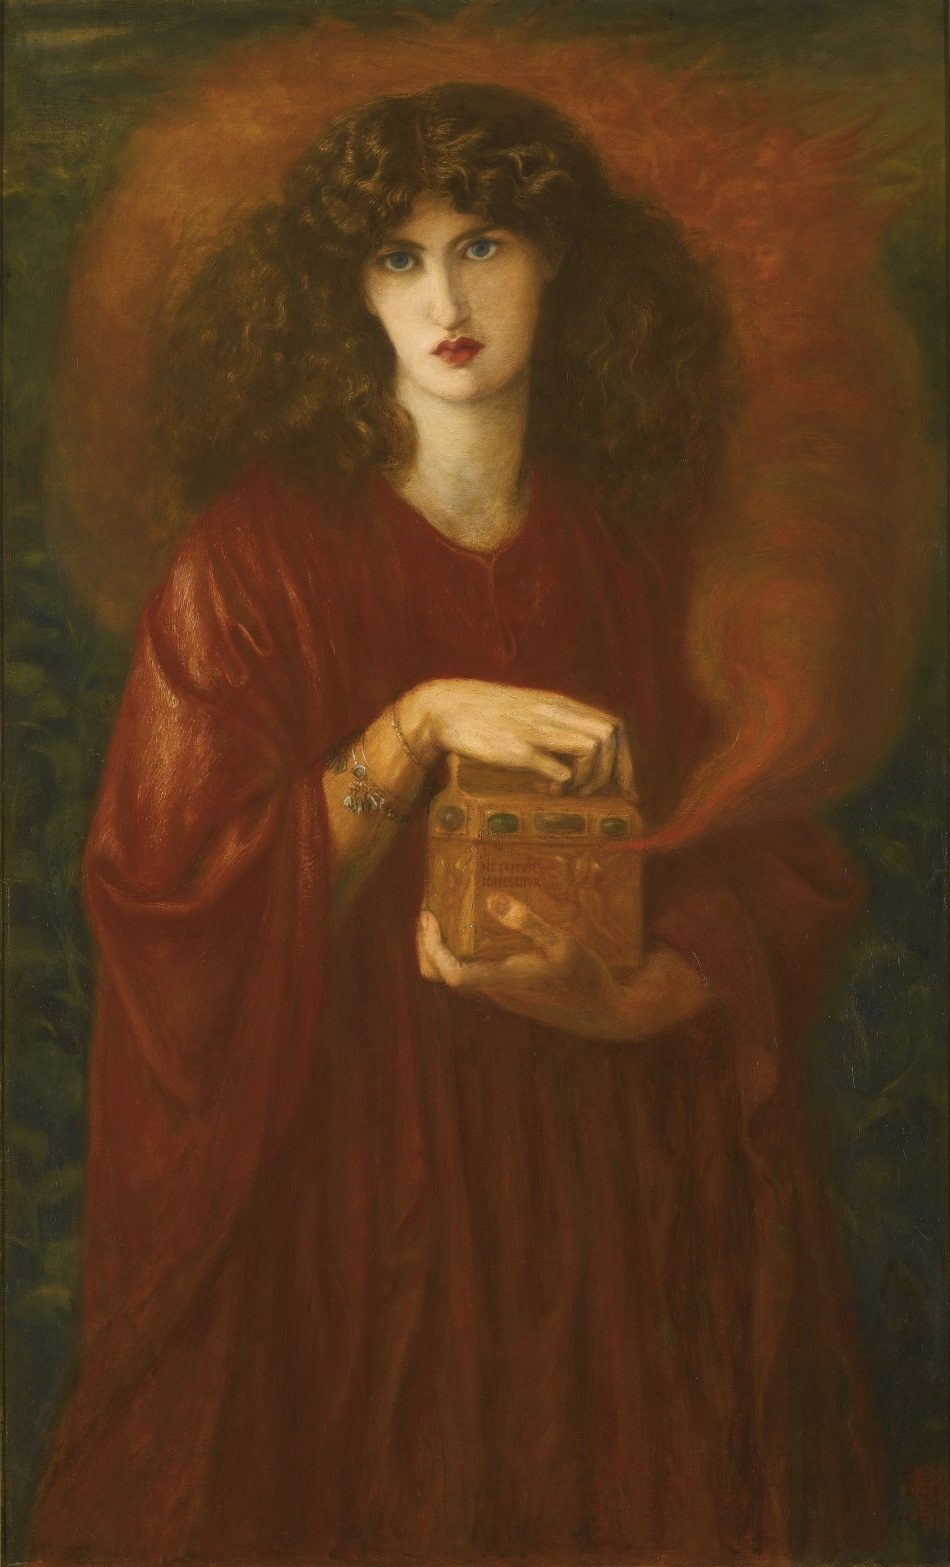
\includegraphics[width=\paperwidth, trim={0 3cm 0 0}]{thesis/6_figures/COVER/Dante_Gabriel_Rossetti_-_Pandora.jpg}%
        }%
    }

    \phantom{.}
    \vfill

    \dusffamily
    
    \fontsize{12}{12}\selectfont 
    MATTIA SOTGIA
    
    {
        \fontsize{45}{45}\selectfont
        \bfseries
        OPENING THE PANDORA JAR\par
        
        \vspace{1em}
        
        \fontsize{15}{25}\selectfont 
        A DEDICATED STUDY OF THE AUTOMATIC EVENT RECONSTRUCTION IN THE ICARUS EXPERIMENT
        % A dedicated study of the automatic event reconstruction in the ICARUS-T600 experiment
    }
\end{titlepage}


% \cleardoublepage

\begin{titlepage}
    \ifdraft\BgThispage\fi
    \begin{center}
        
        {{Università degli Studi di Genova}}\par

        {Scuola di Scienze Matematiche, Fisiche e Naturali} \par

        \vspace{0.5cm}

        {Anno Accademico 2024/2025}

        \vfill

        Tesi di Laurea Magistrale in Fisica\par
        Curriculum di Fisica delle Interazioni Fondamentali

        \vfill

        \begin{minipage}{0.775\linewidth}
            \centering
            \huge
            \bfseries
            {\LARGE Opening Pandora's box}\par%
            {\Large A dedicated study of the automatic event reconstruction in the ICARUS-T600 experiment}%
        \end{minipage}

        \vfill

        \textbf{\small Candidato}\\{Mattia Sotgia}%
%
        \vfill%

        \begin{minipage}{0.45\linewidth}%
            \textbf{\small Relatrice}\par%
            {Dr. Alice Campani}\par\vspace{1em}%
            % {Universit\`a degli studi di Genova}\par\vspace{1em}
            \textbf{\small Relatore}\par%
            {Prof. Marco Pallavicini}%
            % \par{Universit\`a degli studi di Genova}
        \end{minipage}%
        \hfill%
        \begin{minipage}{0.45\linewidth}
            \raggedleft
            \textbf{\small Correlatrice}\par
            {Carla Biggio}
        \end{minipage}

        \vspace{2cm}

		Genova, 15 settembre 2025
        % Genova, 25 ottobre 2025
    \end{center}
\end{titlepage}


\cleardoublepage

\thispagestyle{empty}
\phantom{.}
\vspace{8cm}
\dictum[Wolfgang Pauli]{I have done something very bad today by proposing a particle that cannot be detected; it is something no theorist should ever do.}
\cleardoublepage

% !TEX root = ../main.tex

% \addchap{Abstract}

% \addsec{\@title}

\begin{abstract}
The three-flavor neutrino mixing minimal extension of the Standard Model (SM) has been established by a number of experiments in the past two decades. However, a series of experimental anomalies were observed, indicating a possible hint of the existence of a fourth neutrino, called \emph{sterile neutrino} because it does not undergo weak interaction.

This $3+1$ extension of the SM is the main physics target of the ICARUS experiment as part of the Short-Baseline Neutrino (SBN) program at Fermilab. The ICARUS-T600 760-ton detector is a Liquid Argon Time Projection Chamber (LAr-TPC) successfully employed at the LNGS laboratories for a three-year physics run and now collecting data at Fermi National Accelerator Laboratory (FNAL). The physics program of the ICARUS experiment also includes the measurement of neutrino-Argon cross sections employing the off-axis Neutrino at the Main Injector (NuMI) beam and several Beyond Standard Model studies.

The automatic TPC event reconstruction in ICARUS is performed using the Pandora Pattern Finding Algorithm framework that performs a 3D reconstruction of the image recorded in the collected event, including the identification of interaction vertices and the classification of tracks and showers inside the TPC.

In view of the standalone ICARUS oscillation $\PGnGm\text{CC}$ analysis and of the future combined SBN oscillation analysis, a thorough evaluation of the performances of reconstruction chain, as well as the systematic uncertainties induced on the reconstructed neutrino energy spectrum is essential. The main objective of this work is to evaluate the performances of single steps of the reconstruction sequence, while possibly testing improvements of the machine learning algorithms employed in specific stages of the chain.
\end{abstract}


\frontmatter
% !TEX root = ../main.tex
\chapter*{Acknowledgement}



\begin{flushright}
    \emph{Mattia}\par
    15 ottobre 2025
\end{flushright}
\tableofcontents

\listoffigures

\mainmatter
% !TEX root = ../main.tex

\addchap{Introduction}

% Catchy introduction: neutrino world, something hystorical and so on...
Neutrinos are the most abundant particle in the universe, with billions of neutrinos passing trough each square centimeter each second, primarily coming from our neighbour star, the Sun: within nuclear reactions inside the Sun's core, billions of neutrino are created, and, due to their weakly interactive nature they travel unaltered to Earth. Other neutrino sources are also core-collapse supernovae, interacting cosmic ray within Earth's atmosphere, and, nonetheless, nuclear reactors and accelerator complexes. 

The discovery of neutrino oscillations, hence the evidence for neutrino masses, is a striking proof of Beyond the Standard Model (BSM) physics. 
Generating neutrino masses is qualitatively different from generating masses for any other fermionic particle content of the Standard Model (SM).  
Several are the possible scenarios for introducing neutrino masses in the SM: in general, the mechanism of neutrino masses would require addition of new particle state to the SM that have never been observed. The addition of this particle states would modify substantially neutrino-related observables, and would have effects, for example, on oscillation phenomenology. 

Interest in this direction has been fanned, more recently, by a series of neutrino anomalous measurement at short-baseline oscillation experiments, at accelerating complexes, like the LSND and MiniBooNE collaborations, at Gallium-based experiments, like GALLEX, SAGE and BEST collaborations, and at reactors baselines, like the Neutrino-4 collaboration.

None of these short-baseline experimental anomalies, hovewer, proved to be definitive, even if the global picture shows a strong tension with the current model. An individual program aiming at a $>5\sigma$ sensitivity, on multiple short-baseline oscillation channels experiment is needed to test these results and draw a complete picture for these short-baseline experimental anomalies. 

The Short Baseline Neutrino (SBN) program at Fermilab is a three detector, short-baseline, multiple oscillation channel experimental effort, located along the Booster Neutrino Beam (BNB) baseline. All the three detectors in the beamline are Liquid Argon Time Projection Chambers (LArTPC(s)), exploiting on the high precision calorimetric power and mm-scale three dimensional tracking capabilities of such detectors to archive unprecedented sensitivity on the sterile neutrino search. 

The ICARUS T600 detector acts as the SBN Far Detector (SBN-FD) at a baseline of \SI{600}{\meter}.
The location of both the ICARUS detector and of the SBN Near Detector, SBND, where chosen to optimize neutrino oscillation sensitivity and minimize the impact of flux systematics. Among the Booster Neutrino Beam, the ICARUS T600 detector is also on the baseline of the Neutrino from the Main Injector (NuMI) Beam, crossing the detector $\SI{6}{\degree}$ off-axis wih respect to the detector principal axis. 
The ICARUS detector is now finishing its fourth physics run, three of which were done while the SBN near detector was preparing to start its physic operation. With all this data the collaboration has started to look into $\PGnGm$-disappearance studies, with the simplest topologies being $1\PGm1\Pp$ and $1\PGm N\Pp$. 

% Thesis main goal, supported by nothing else than the idea
In order to reduce the systematic uncertainties related to the reconstruction efficiency, a detailed study of the event reconstruction inside the ICARUS TPC is needed, alongside an effort to align the ICARUS and SBND detectors signal processing and event reconstruction chain, in view of the future SBN joint analysis. 

Of all steps involved in the event processing and reconstruction, one of great importance is related to the particle objects building from the signals left on the wireplanes, and the subsequent event hierarchy creation (that is defining which are the primary particles originating from the interaction vertex and the interaction \emph{structure}), which is the centerpiece of many further analysis. 
This process is performed by a set of algorithms shared across the LArTPC technology detectors. The common framework is based on the Pandora Patter Finding Algorithm software. This feature, alongside the various algorithms suited for the reconstruction, a set of tools that can be used to perform studies on the reconstruction efficiency, previously unused by the ICARUS collaboration. 

The goal of this thesis is to validate this set of tools for further use in the ICARUS collaboration, and show their power by performing a detailed efficiency analysis of the TPC reconstruction chain. 
This will likely serve both as a validation for the current analysis, as wall as a foundation for later works --- such as the future $\PGne$-appearance analysis --- where these tools can be used to validate the reconstruction for the shower-like particles, where the reconstruction hit a big wall due to the particle-argon interaction topology and the signal that it produces. 

% Thesis structure
The thesis structure is as follows\begin{itemize}
    \item \autoref{chap:theory_introduction} is devoted to introducing the theoretical framework of the Standard Model of Particle Physics, with a great interest on the physics of neutrinos, their \emph{classical} picture, the phenomenology of neutrino oscillator behaviour and some of the anomalies driving the sterile neutrino picture. 
    \item \autoref{chap:icarus_detector} tries to get a detailed description of the ICARUS T600 detector, its three sub-systems, the Liquid Argon Time Projection Chamber, the light collection system and the cosmic ray tagging system, and its role in the Fermilab Short Baseline Neutrino Program. 
    \item \autoref{chap:event_reconstruction} is dedicated to an overview of the event reconstruction in all the T600 sub-detectors, with a primary focus on the TPC event reconstruction. 
\end{itemize}


% !TEX root=../main.tex

\chapter{Active and sterile neutrinos}

% !TEX root = ../main.tex

\chapter{The SBN program at Fermilab and the ICARUS experiment}
\label{chap:icarus_detector}

\section{The Short Baseline Neutrino program at Fermilab}
%% BRIEF INTRODUCTION
The Short Baseline Neutrino experimental program at Fermi National Accelerator Laboratories aims to  draw a complete and consistent picture of the sterile neutrino scenario, depicted in detail in \autoref{chap:theory_introduction}. 
% The main physics goal of the SBN collaboration is to test with great sensitivity the presence of a fourth sterile neutrino state, as suggested by multiple experimental anomalies. 
To achieve a level of statistical significance greater than $5\sigma$ for the LSND-allowed region (at \SI{90}{\percent} CL), SBN will carry out precision searches, recording millions of NC and CC neutrino interactions on argon. 

The key to such high sensitivity, other than the great statistic of events collected, is the design paradigm of the program. It will employ the Liquid Argon Time Projection Chamber (LArTPC) technology \cite{rubbiaLiquidArgonTime1977}, with two functionally identical detectors placed at different distances from the neutrino source. This way, the oscillatory behaviour is observed by comparing the neutrino flux at the far detector with the ``control'' flux recorded at the near detector, reducing the systematic uncertainties related to neutrino production and neutrino interaction in argon. 

Albeit the original plan for a three-detector program \cite{acciarriProposalThreeDetector2015}, MicroBooNE finished its data-taking period in 2020, two years prior to ICARUS starting its data collection campaign and five prior to SBND, so the SBN program will perform a search for the sterile neutrino as a two-detector experiment \cite{acciarriProposalThreeDetector2015, machadoShortBaselineNeutrinoProgram2019}. 

Both collect data from the common Booster Neutrino Beam (BNB); additionally, the ICARUS detector is located such that it is sensible to off-axis neutrinos coming from the Neutrino at the Main Injector (NuMI) beam. 

ICARUS is the far detector for the SBN programme, employing an active mass of \SI{476}{\tonne} of liquid argon (LAr), at a distance of \SI{600}{\meter} from the neutrino source; its position was chosen so as to maximise the oscillation probability. The ICARUS detector started its data taking independently from the SBN program in June of 2022, after the initial commissioning phase. It has now finished the fourth data collection campaign, collecting $\sim \SI{7.54e20}{POT}$ (proton-on-target), corresponding to about \num{e6} neutrino events.

At a distance of \SI{110}{\meter}, SBND is the near detector of the SBN program, with an active LAr mass of \SI{112}{\tonne}. After commissioning, it started data taking in December of 2024, joining the far detector and allowing for a precise knowledge of the neutrino flux. 

\paragraph{Oscillation measurements with a two-detector experiment} The main physics goal of the SBN program is the search for a fourth sterile neutrino state in the $3+1$ model. Using multiple LArTPC detectors, a high-sensitivity search for a high-$\Delta m^2$ splitting is possible by studying muon-neutrino oscillations in the $\PGnGm\to\PGnGm$ disappearance and $\PGnGm\to\PGne$ appearance channels. 

\begin{figure}
    \centering
    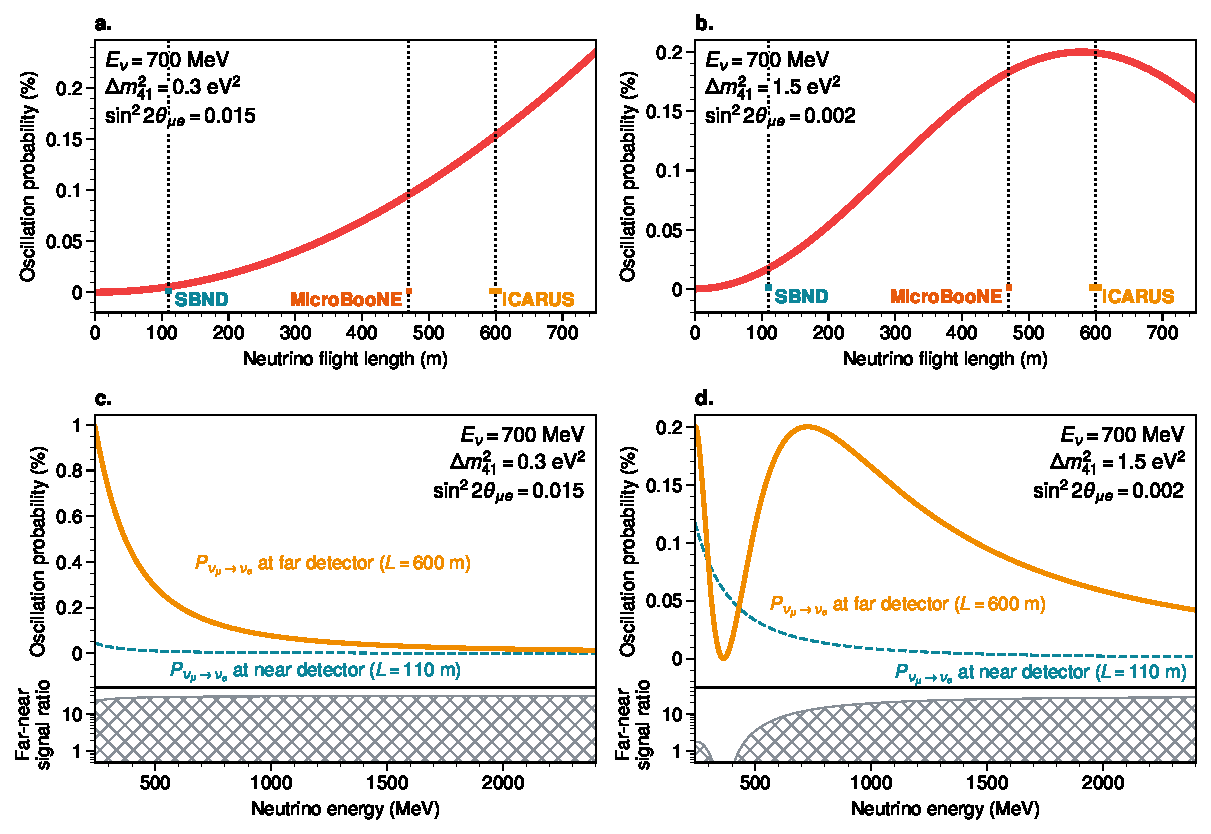
\includegraphics[width=\linewidth]{SBN_sensitivity/appearance_signal.pdf}
    \caption[Electron neutrino appearance probability in the $3+1$ sterile oscillation scenario]{(a) and (b) show the oscillation probability for a \SI{700}{MeV} muon neutrino into an electron neutrino as a function of the length of the neutrino flight using two benchmark values of $(\sin^22\theta_{\PGm\Pe}, \Delta m^2)$. (c) and (d) show the same oscillation probability as a function of the neutrino energy. Additionally, the bottom panels show the far-over-near ratio. Adapted from \cite{machadoShortBaselineNeutrinoProgram2019}.}
    \label{fig:oscillation_2body_SBN}
\end{figure}

The oscillation probability for both channels is presented in \eqref{eq:2body_oscillation_sterile_disapp} and \eqref{eq:2body_oscillation_sterile_app} for the disappearance and appearance channels, respectively, with the assumption of the $3+1$ model. Looking at the $\PGnGm\to\PGne$ appearance channel, from the experimental results shown in \autoref{fig:all_experimental_searches}, the allowed parameter space lies in $\sin^22\theta_{\PGm\Pe} \in (\num{e-3},\num{e-1})$ and $\Delta m^2 \in (\num{e-1}, \num{e1})\ \si{eV^2}$; the location of the near and far detector  has been optimised to maximise the oscillation probability in this region of parameters. \autoref{fig:oscillation_2body_SBN} show $P(\PGnGm \rightarrow \PGne)$ for two benchmark values of $(\sin^22\theta_{\PGm\Pe}, \Delta m^2)$, assuming a neutrino energy of $\sim\SI{700}{MeV}$. Exploiting the strong correlations between the fluxes collected at the near and far detectors --- both use the same interaction medium and functionally identical revelation techniques --- the major impacting systematic uncertainties, which are those arising from the production mechanisms and the $\PGn$-Ar interaction cross-sections, can be mitigated in the two-detector configuration. 

With a planned collected statistics of \SI{6.6e20}{POT}, the $\PGnGm\to\PGnGm$ disappearance channel can also be probed to search for neutrino oscillation mediated by a sterile state. The unitarity of the $3+1$ PMNS matrix has to be preserved so that in the event of $\PGnGm\to\PGne$ appearance, meaning a nonzero value of $\sin^22\theta_{\PGm\Pe}$, a nonzero value of $\sin^22\theta_{\PGm\PGm}$, or a $\PGnGm\to\PGnGm$ disappearance signature, should be observed. 

Both channels will be studied to either pinpoint the correct $(\sin^22\theta, \Delta m^2)$ values or exclude some regions in the parameter space. \autoref{fig:sbn_2det} shows the projected excluded and allowed regions of the parameter space in both the \ref{sub@fig:nue_app_sbn_2det} $\PGne$-appearance and \ref{sub@fig:numu_disapp_sbn_2det} $\PGnGm$-disapperance channels of the two-detector operation of the SBN experiment. It should be noted that the projected \SI{6.6e20}{POT} was the original plan that was presented in the experiment proposal \cite{acciarriProposalThreeDetector2015}; however, BNB will operate until 2027, allowing the ICARUS detector to collect three times the statistics in standalone operation. 

\begin{figure}
    \centering
    \subfloat[]{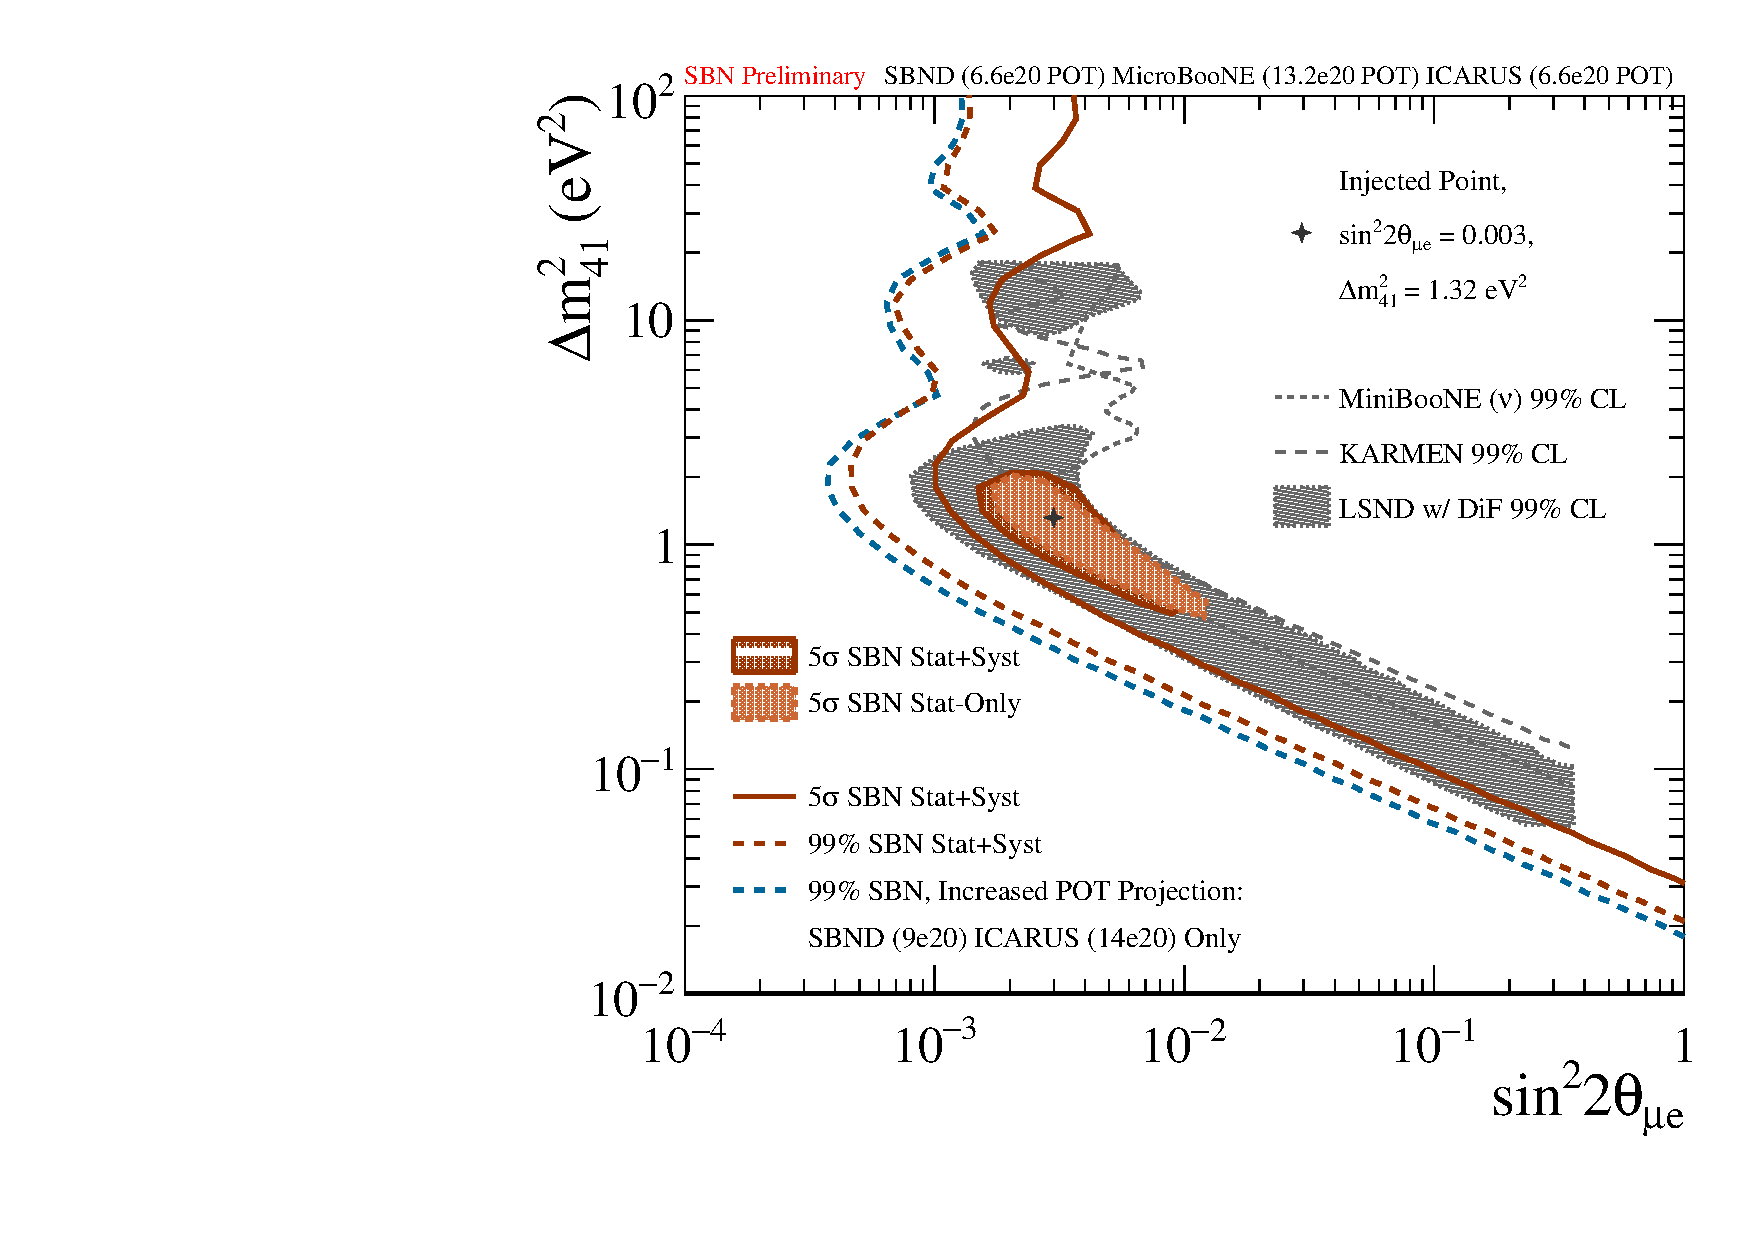
\includegraphics[width=0.5\linewidth]{SBN_sensitivity/nue_app_2det_newPOT_sensitivity_comparison.pdf}\label{fig:nue_app_sbn_2det}}
    \subfloat[]{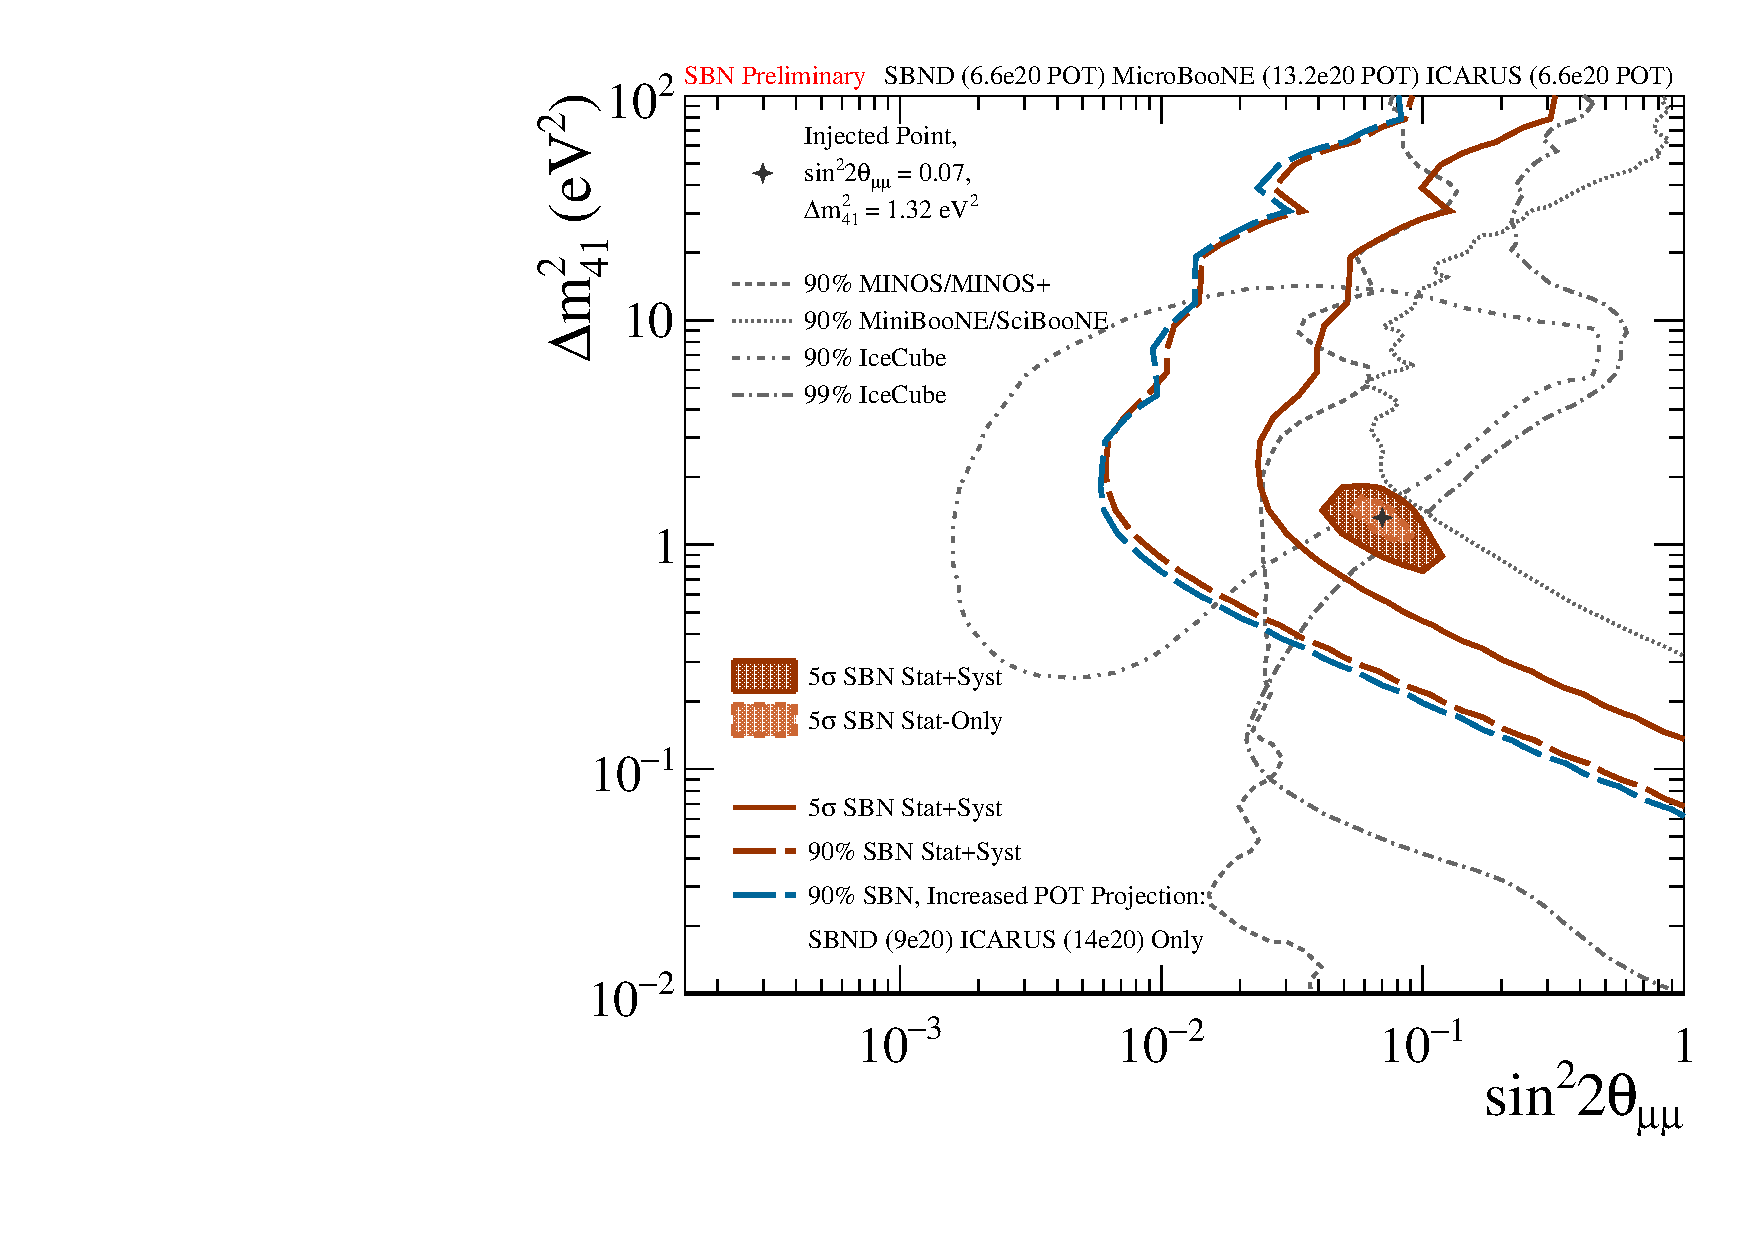
\includegraphics[width=0.5\linewidth]{SBN_sensitivity/numu_disapp_2det_newPOT_sensitivity_comparison.pdf}\label{fig:numu_disapp_sbn_2det}}
    \caption[SBN sensitivity plots in both appearance and disappearance channels]{\ref{sub@fig:nue_app_sbn_2det} and \ref{sub@fig:numu_disapp_sbn_2det} show, respectively, the expected sensitivity curves in the $\PGne$-appearance and $\PGnGm$-disappearance channels under the hypothesis of no observation (solid and dashed lines, respectively at $5\sigma$ and 99\% CL) and under the hypothesis of observing an oscillatory signature in both channels (filled regions). These projections account for a collected \SI{6.6e20}{POT} and a two-detector configuration. }
    \label{fig:sbn_2det}
\end{figure}

Additionally, since a nonzero value of both $\sin^2 2\theta_{\PGm\Pe}$ and $\sin^22\theta_{\PGm\PGm}$ leads to a nonzero value of $\sin^22\theta_{\Pe\Pe}$, both the ICARUS detector, making use of the Booster and NuMI neutrino beams, and the SBND detector, only with data from the Booster beam, will explore the $\PGne$-disappearance channel $\PGne\to\PGne$. The combined result of this multi-channel search will provide strong evidence in favour of or against the $3+1$ sterile neutrino scenario. 

\paragraph{Cross-sections and BSM physics} In addition to the primary physics goals, the SBN programme, with its two LArTPC detectors, delivers a rich physics opportunity. 

Starting from particle interaction in liquid argon, both SBND and ICARUS detectors will use the Booster and NuMI (ICARUS-only) neutrino beams to perform cross-section measurements, exploiting the great amount of collected data with both detectors. 
For SBND, the proximity with respect to the neutrino source leads to a very large flux collected by the detector --- each run approximately of \SI{2.2e20}{POT} corresponds to 1.5M $\PGnGm$ and \num{12000} $\PGne$s; 
the same measurements can be performed with the ICARUS detector, which at the moment benefits from a longer data collection period and an accumulated statistic of \SI{7.5e20}{POT} in standalone operation. The larger dimension of the ICARUS detector also allows for more contained events, where all the final state interactions (FSI) are contained inside the detector active volume, allowing for a better particle identification (PID). 
Additionally, the position of the ICARUS detector allows the collection of neutrinos from the NuMI beam at an off-axis angle of \SI{6}{\degree} with respect to BNB direction. 
The added value of the NuMI beam comes from the energy range it covers. 
Using protons from the Main Injector at an energy of \SI{120}{GeV}, it is able to cover the \qtyrange{1}{3}{GeV} energy range, which overlaps greatly with the DUNE operational energy range. Neutrinos from the NuMI beam will also feature an enriched electronic component from the three-body decay of the kaon, allowing for precise $\PGne$ cross-section measurements. At the moment of writing this thesis, two $\PGnGm$ charged current mesonless cross-section analyses, $\PGnGm\mathrm{CCN>1}\Pp0\PGp$ and $\PGnGm\mathrm{CCN}\Pp0\PGp$, are being carried on and are in the final phases before publication. 

Finally, exploiting the great tracking and calorimetric power of liquid argon TPCs, with exceptional precision and high-performance event reconstruction capabilities, opens up invaluable opportunities for new physics searches. Using high-intensity neutrino beams, with large statistics, it is possible to explore beyond standard model theories. A detailed description of possible searches is presented in refs. \cite{machadoShortBaselineNeutrinoProgram2019, acciarriProposalThreeDetector2015}. 
Recently the first physics paper by the ICARUS collaboration was published, exploring some of these BSM models involving the scalar sector using data from the NuMI beam \cite{icaruscollaborationSearchHiddenSector2025}. 

\subsection{Neutrino beam}

The location for the SBN programme was selected to make use of the already existing accelerator infrastructure at Fermilab. \autoref{fig:accelerator_complex} shows the FNAL accelerator complex schematic overview. This complex provides a powerful beam of neutrinos using protons extracted from the Booster accelerator, core to the operation of the SBN experiment, as well as multiple other particle beams (neutrinos and muons, as well as protons) which are employed in other experiments, such as the Neutrinos at the Main Injector Beam. 

The common starting point is the Linac (linear accelerator), boosting protons up to \SI{400}{MeV} of energy (or $\sim\SI{954}{MeV}$ of momentum) using radiofrequency (RF) cavities. Accelerated protons are extracted and boosted to an energy of \SI{8}{GeV} within the Booster ring. 

\begin{figure}
    \centering
    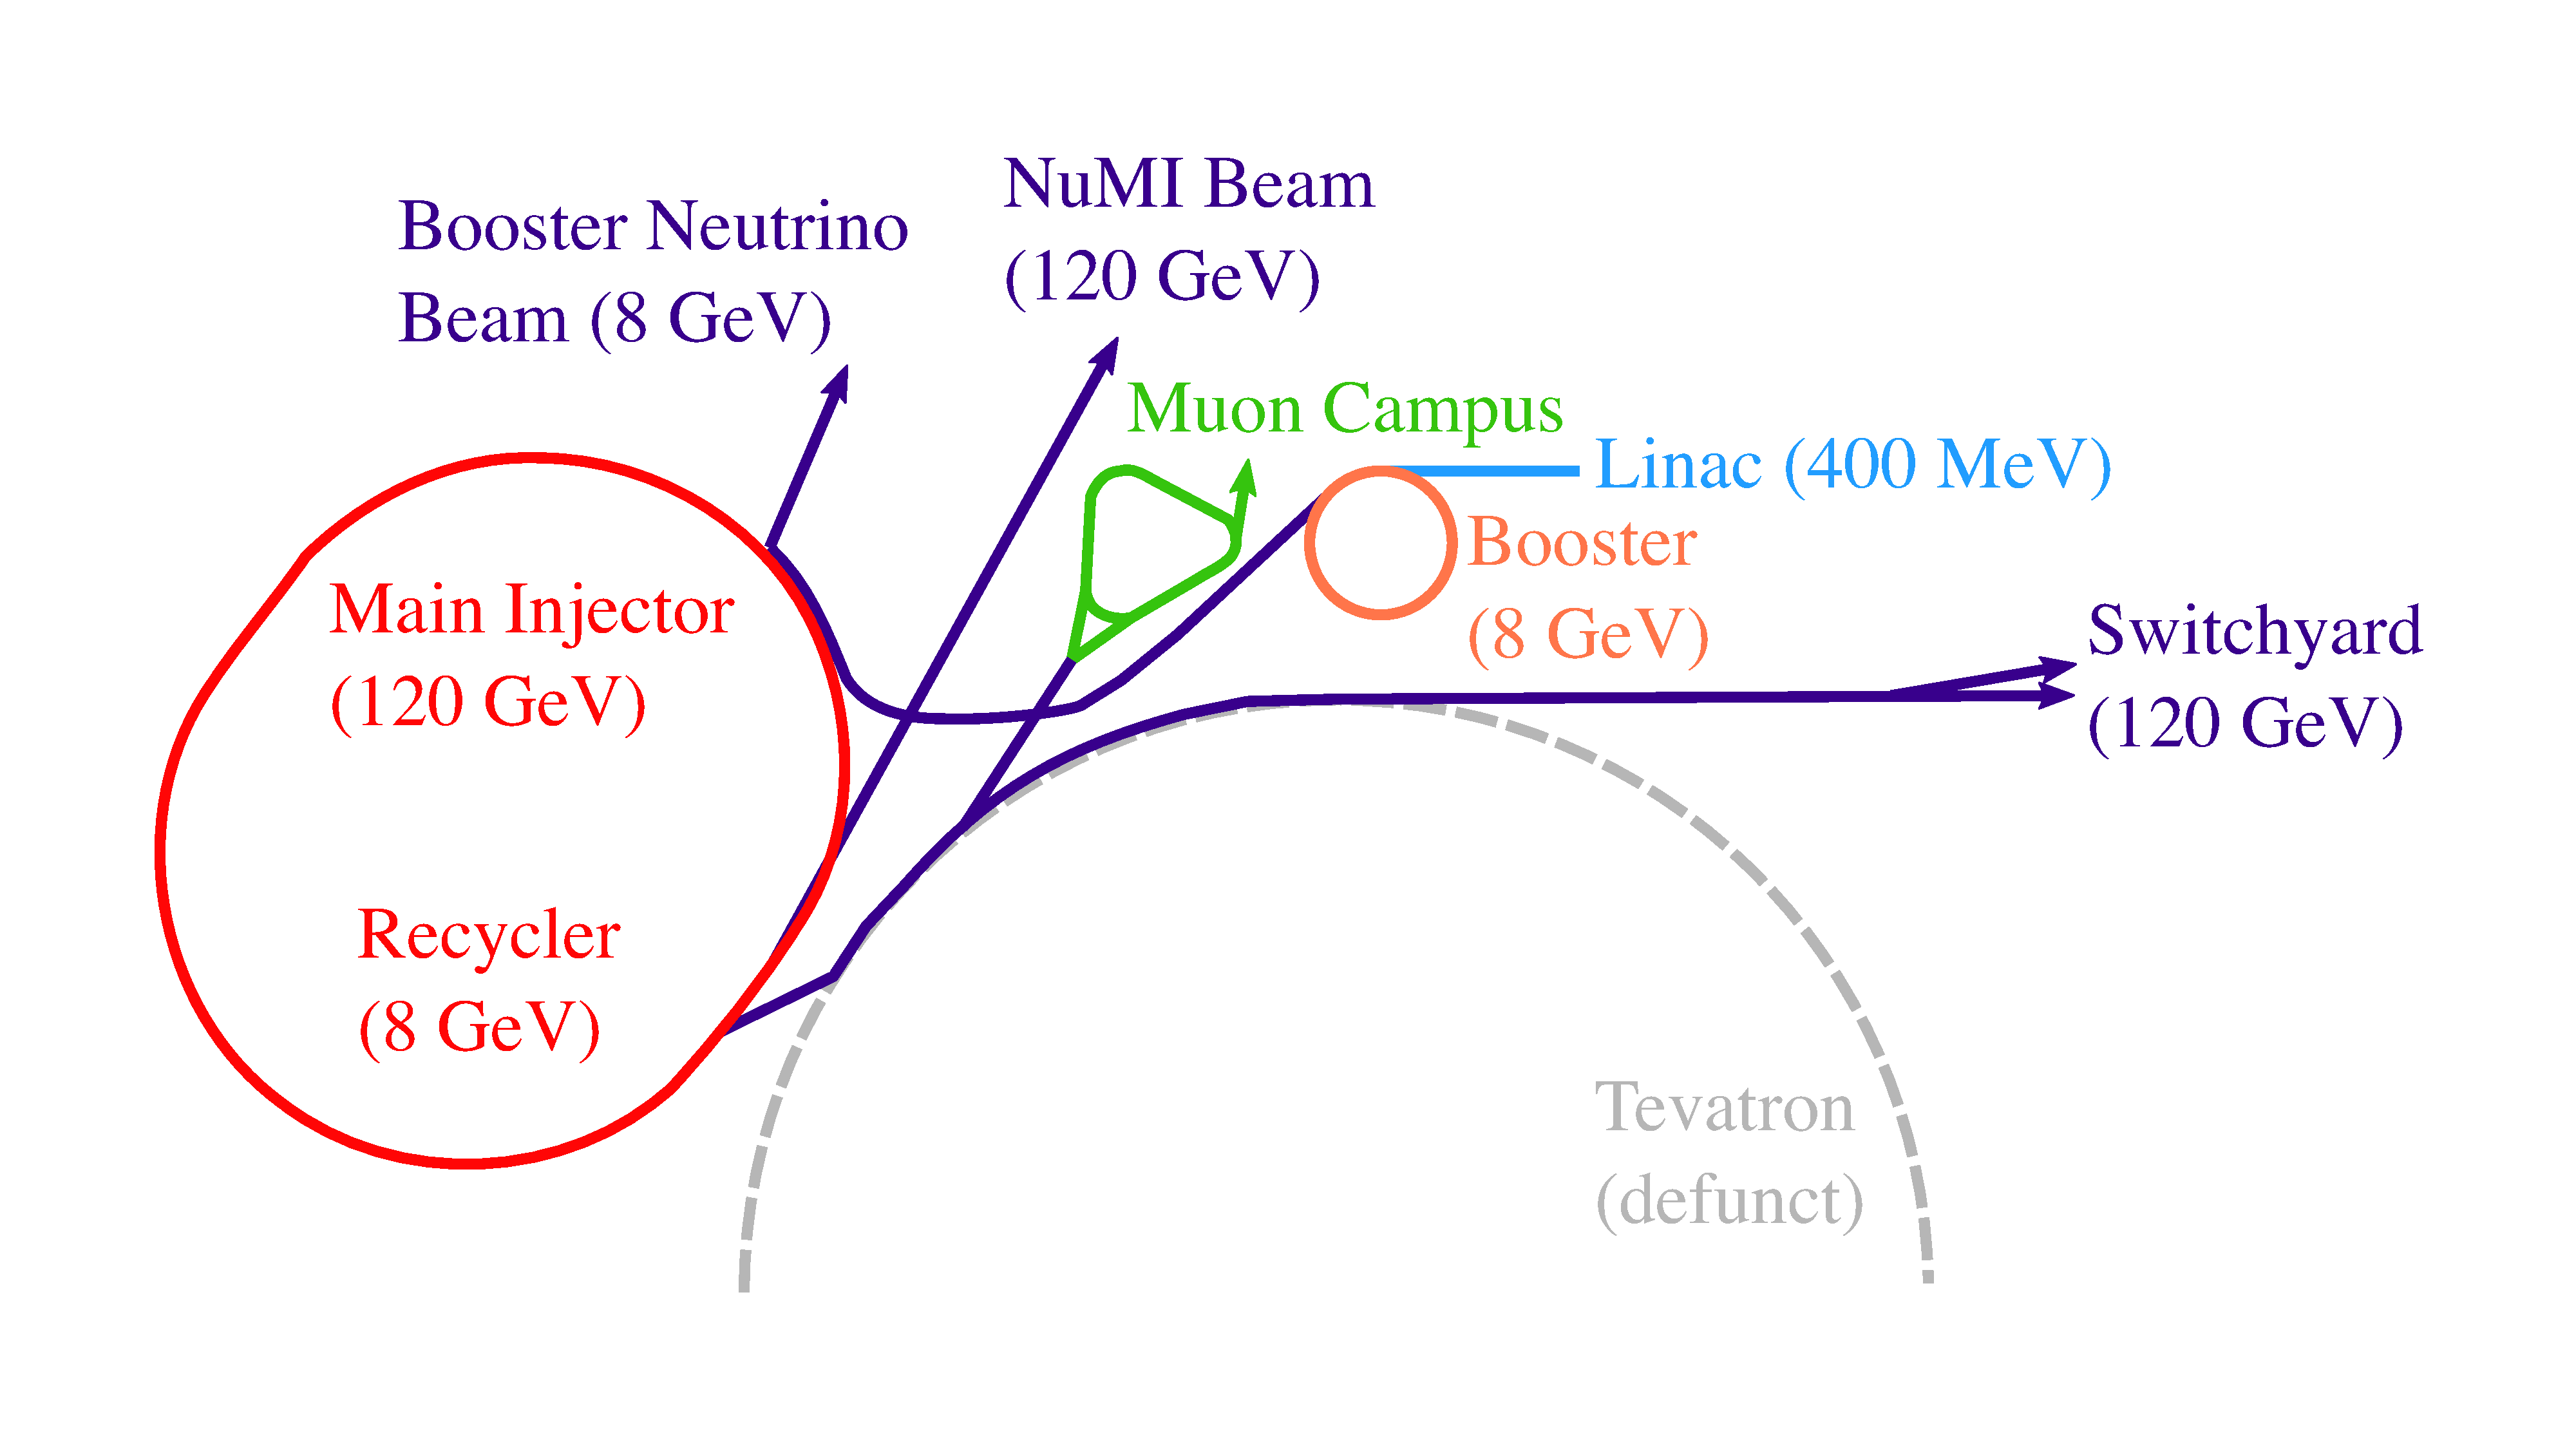
\includegraphics[width=0.75\linewidth]{detector/BNB_NuMI_beams.pdf}
    \caption[Fermilab Accelerator complex]{Schematics of the accelerator complex at Fermilab. Both Booster and NuMI neutrino beams serve the ICARUS detector, with different energy  ranges, \SI{700}{MeV} for BNB and \SI{2.5}{GeV} for NuMI. Taken from \cite{ainsworthHighIntensityOperation2020}.}
    \label{fig:accelerator_complex}
\end{figure}

From the Booster ring, a fraction of protons is extracted to be used for the Booster Neutrino Beam, whereas the remaining fraction is sent into the Main Injector accelerator. From there a second Neutrino beam is extracted, the Neutrinos at the Main Injector (NuMI) beam. 

\begin{figure}
    \centering
    \subfloat[]{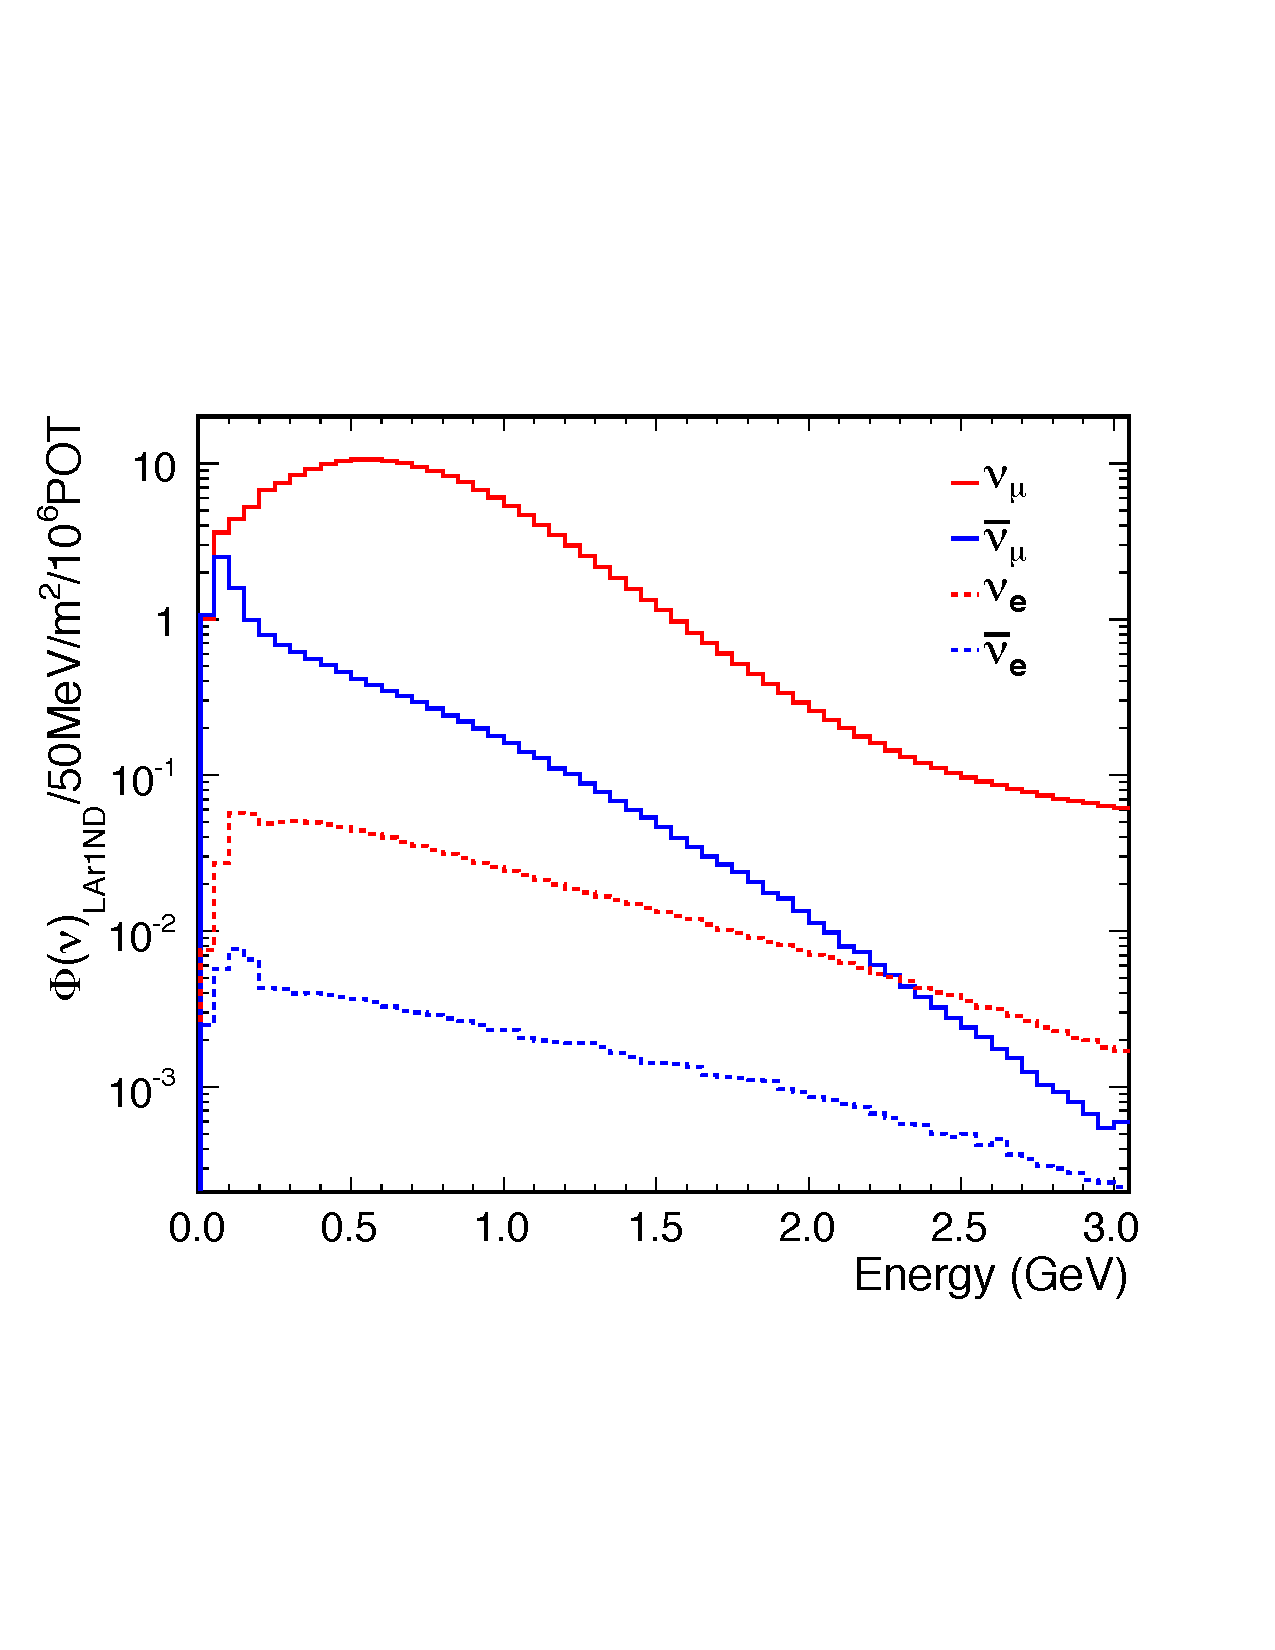
\includegraphics[trim={0 6cm 0 6cm}, width=0.5\linewidth]{beams/BNB_flux_lar1nd.pdf}\label{fig:BNB_flux_SBND}}
    \subfloat[]{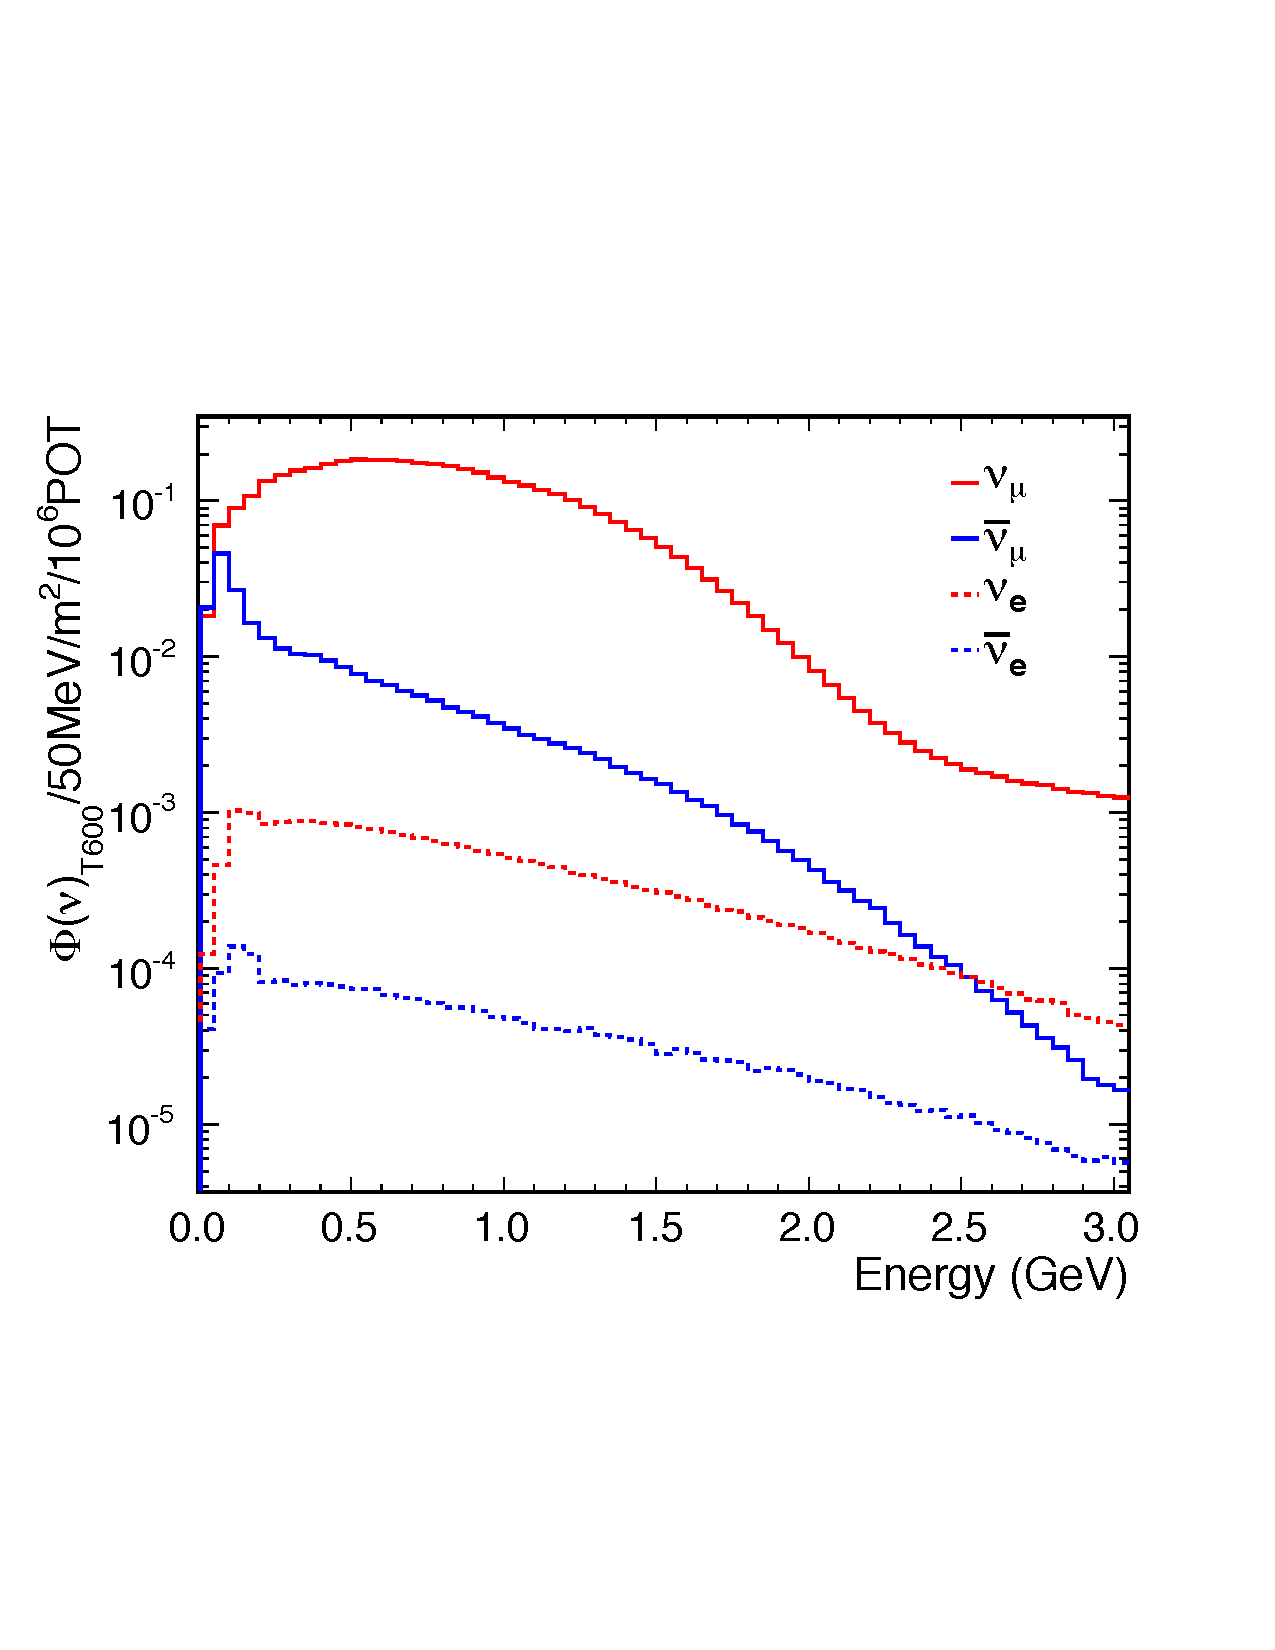
\includegraphics[trim={0 6cm 0 6cm}, width=0.5\linewidth]{beams/BNB_flux_icarus.pdf}\label{fig:BNB_flux_ICARUS}}

    % \subfloat[]{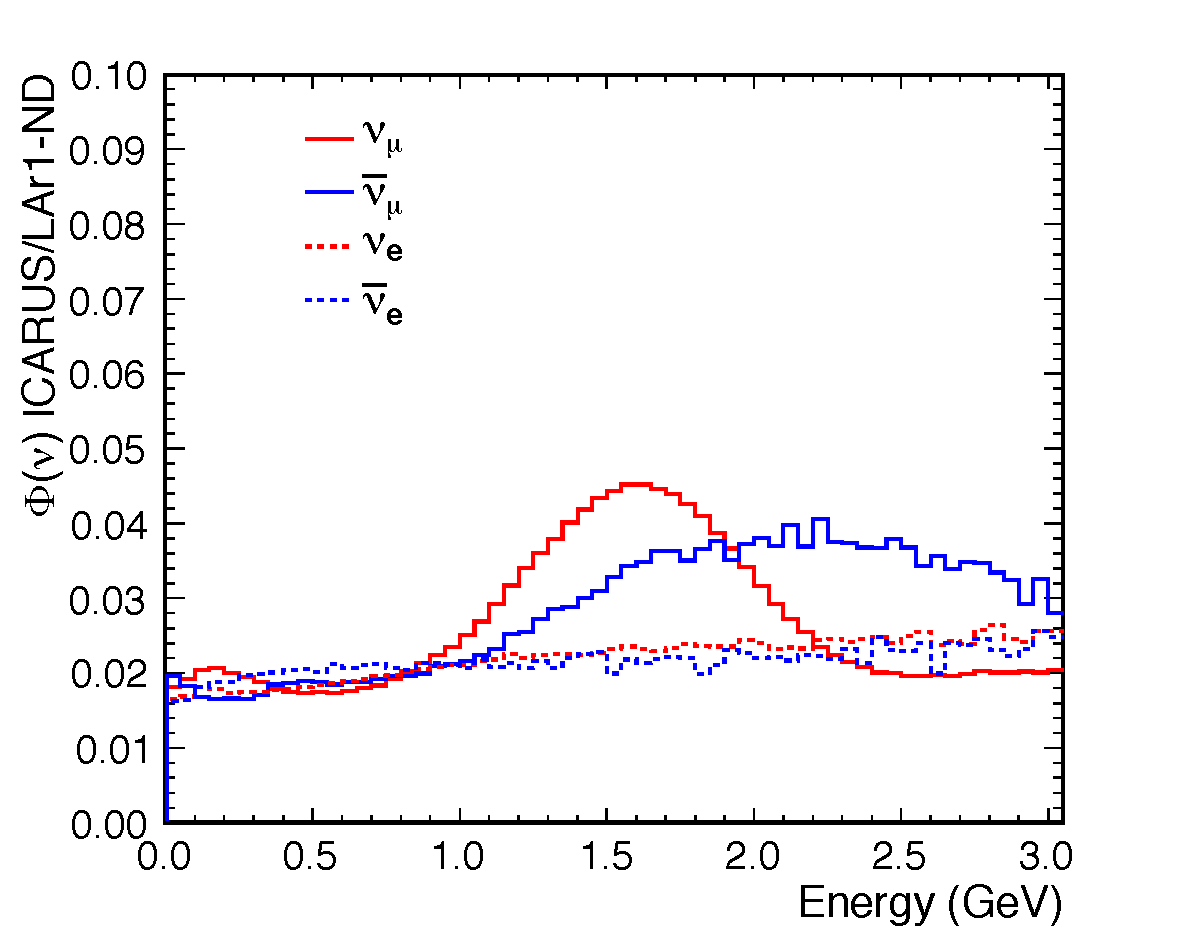
\includegraphics[trim={0 0cm 0 0cm}, width=0.5\linewidth]{thesis/6_figures/beams/BNB_flux_ratio_icarus_lar1nd.pdf}\label{fig:BNB_flux_ICARUS_SBND_ratio}}
    \caption[BNB flux predictions at the near and far detectors]{Predictions of the neutrino flux as computed by the MicroBooNE collaboration \cite{miniboonecollaborationNeutrinoFluxPrediction2009} at distances of \SI{110}{m} \ref{sub@fig:BNB_flux_SBND} and \SI{600}{m} \ref{sub@fig:BNB_flux_ICARUS} from the beryllium target, i.e., for the SBND and ICARUS detectors, respectively. Taken from \cite{acciarriProposalThreeDetector2015}. }
    % \ref{sub@fig:BNB_flux_ICARUS_SBND_ratio} shows the predicted ratio of the two fluxes under the hypothesis of no sterile-mediated oscillation anomaly. }
    \label{fig:BNB_flux}
\end{figure}

\paragraph{Booster Neutrino Beam} Protons accelerated up to \SI{8}{GeV} inside the Booster ring are extracted in groups of 81 bunches, each wide $\sim\SI{2}{ns}$ and \SI{19}{ns} apart. The repetition rate for the extraction, mainly limited by the focusing horn power supply, is of \SI{5}{\hertz}. Each pulse collides \SI{5e12}{p} onto a beryllium target. The target is embedded within a pulsed electromagnet (the ``horn'') that produces a toroidal magnetic field to focus positive secondary particles and defocus negative secondary particles emerging from proton-beryllium interactions. Charged mesons, which constitute the majority of the secondary particles emerging from $\Pp$-Be interaction, decay in a 50-meter-long decay region. Within the decay region, charged pions undergo weak decay \begin{equation}
    \PGppm \to \PGmpm + \brabar\PGnGm, \label{eq:pion_decay}
\end{equation} resulting in an (anti)neutrino beam. The length of the decay pipe was chosen so as to maximise the muon (anti)neutrino content and minimise the electron (anti)neutrino content coming from the decay of secondary muons \begin{equation}
    \PGmpm \to \Pepm + \brabar \PGnGm + \brabar \PGne \label{eq:muon_decay}
\end{equation} at $\sim \SI{0.5}{\percent}$ level. Neutrinos produced by BNB have a most probable value for the energy at $E_\PGn\simeq \SI{700}{MeV}$, and a maximum energy around \SI{2.5}{GeV}. When the beam is in FHC (forward horn current, selecting primarily positive mesons), the beam composition is dominated by muon neutrinos $\sim\SI{93.6}{\percent}$, with neutrinos coming from pion decay and kaon decay for neutrinos with energies greater than \SI{2}{GeV}; the second major component is given by $\PAGnGm$ coming mainly from not-defocused $\PGpm$ \eqref{eq:pion_decay} and decaying muons \eqref{eq:muon_decay}; the same decay accounts for, together with neutral kaon decays, an intrinsic $\sim\SI{0.5}{\percent}$ fraction of $\PGne + \PAGne$. 

A detailed study of the beam profile and composition, to allow for precise simulations, was performed by the MiniBooNE collaboration \cite{miniboonecollaborationNeutrinoFluxPrediction2009}, and experimentally verified using the Hadron Production Experiment (HARP). \autoref{fig:BNB_flux} shows the beam fractional composition as a function of the energy of the neutrino. 

\paragraph{Neutrinos at the Main Injector off-axis beam} Once protons are accelerated within the Booster ring, they are then transferred inside the Main Injector ring. There protons are accelerated up to an energy of \SI{120}{GeV}. The MI circumference is roughly seven times that of the Booster ring, so it can hold up to seven entire Booster cycles in it. However, to make space for the pulse kicker rise time, only six are filled, adding up the spill time to \SI{9.5}{\micro\second}: in such time window, NuMI is able to provide a flux of \SI{6.5e13}{POT}. Protons are collided against a graphite target, and produced mesons decay inside a \SI{675}{\meter} long decay tunnel. As for BNB, the main decay products are \eqref{eq:pion_decay} muons and muon neutrinos, with a small fraction of muon antineutrinos and electron neutrinos. 

ICARUS is, however, detecting neutrinos from NuMI at an off-axis angle of $\sim\SI{5.7}{\degree}$ with respect to the detector $z$ coordinate, corresponding to BNB direction. This changes drastically the composition of the beam detected by ICARUS, as off-axis neutrinos and antineutrinos have pretty much the same flux, and overall the fraction of electron (anti)neutrinos is larger. This different beam composition, added to the fact that the energy range is higher than BNB energy range, peaking at \SI{1.5}{GeV} and extending up to \SI{4}{GeV}, allows NuMI to be crucial for ICARUS operations: higher energies overlap better with the expected energy spectrum of future experiments, as for example the DUNE experiment, whilst a greater fraction of electron neutrinos allows for the study of both muon- and electron-neutrino argon interaction cross-sections. Additionally, off-axis detection is core for BSM physics searches since it allows to probe the decay of high-energy mesons at high angles with respect to the beam direction. This is the case, for example, for the first physics paper published by the ICARUS collaboration at Fermilab, looking at di-muon final state topologies to probe the existence of long-lived particles (LLPs) in kaon decays involving a di-muon FSI, $\PK \to \PGp + \mathrm{LLP}(\to \PGm\PGm)$ \cite{icaruscollaborationSearchHiddenSector2025}. 

\section{Liquid Argon Time Projection Chambers} 

Core to the high sensitivity of the SBN programme is the shared Liquid Argon Time Projection Chamber technology between the two functionally identical near and far detectors, respectively the SBND and ICARUS detectors. The Time Projection Chamber technology was first proposed by David R. Nygren \cite{Marx:1978zz}. This technology, whose working principle is pictured in \autoref{fig:TPC}, allows both 3D reconstruction as well as calorimetric capabilities. The basic idea of a TPC detector is that of a large volume, filled with gas or liquid, acting as the interaction medium. Charged particles interact inside this volume, producing ionisation pairs. Free electrons produced in the ionisation process are drifted by means of a strong electric field from the cathode toward the anode, where the ionisation electron charge information is collected by a position-sensitive plane, providing one or more 2D projections of the interaction. The drifting time is used as the third missing component to perform 3D event reconstruction inside the detector. 

\begin{figure}
    \centering
    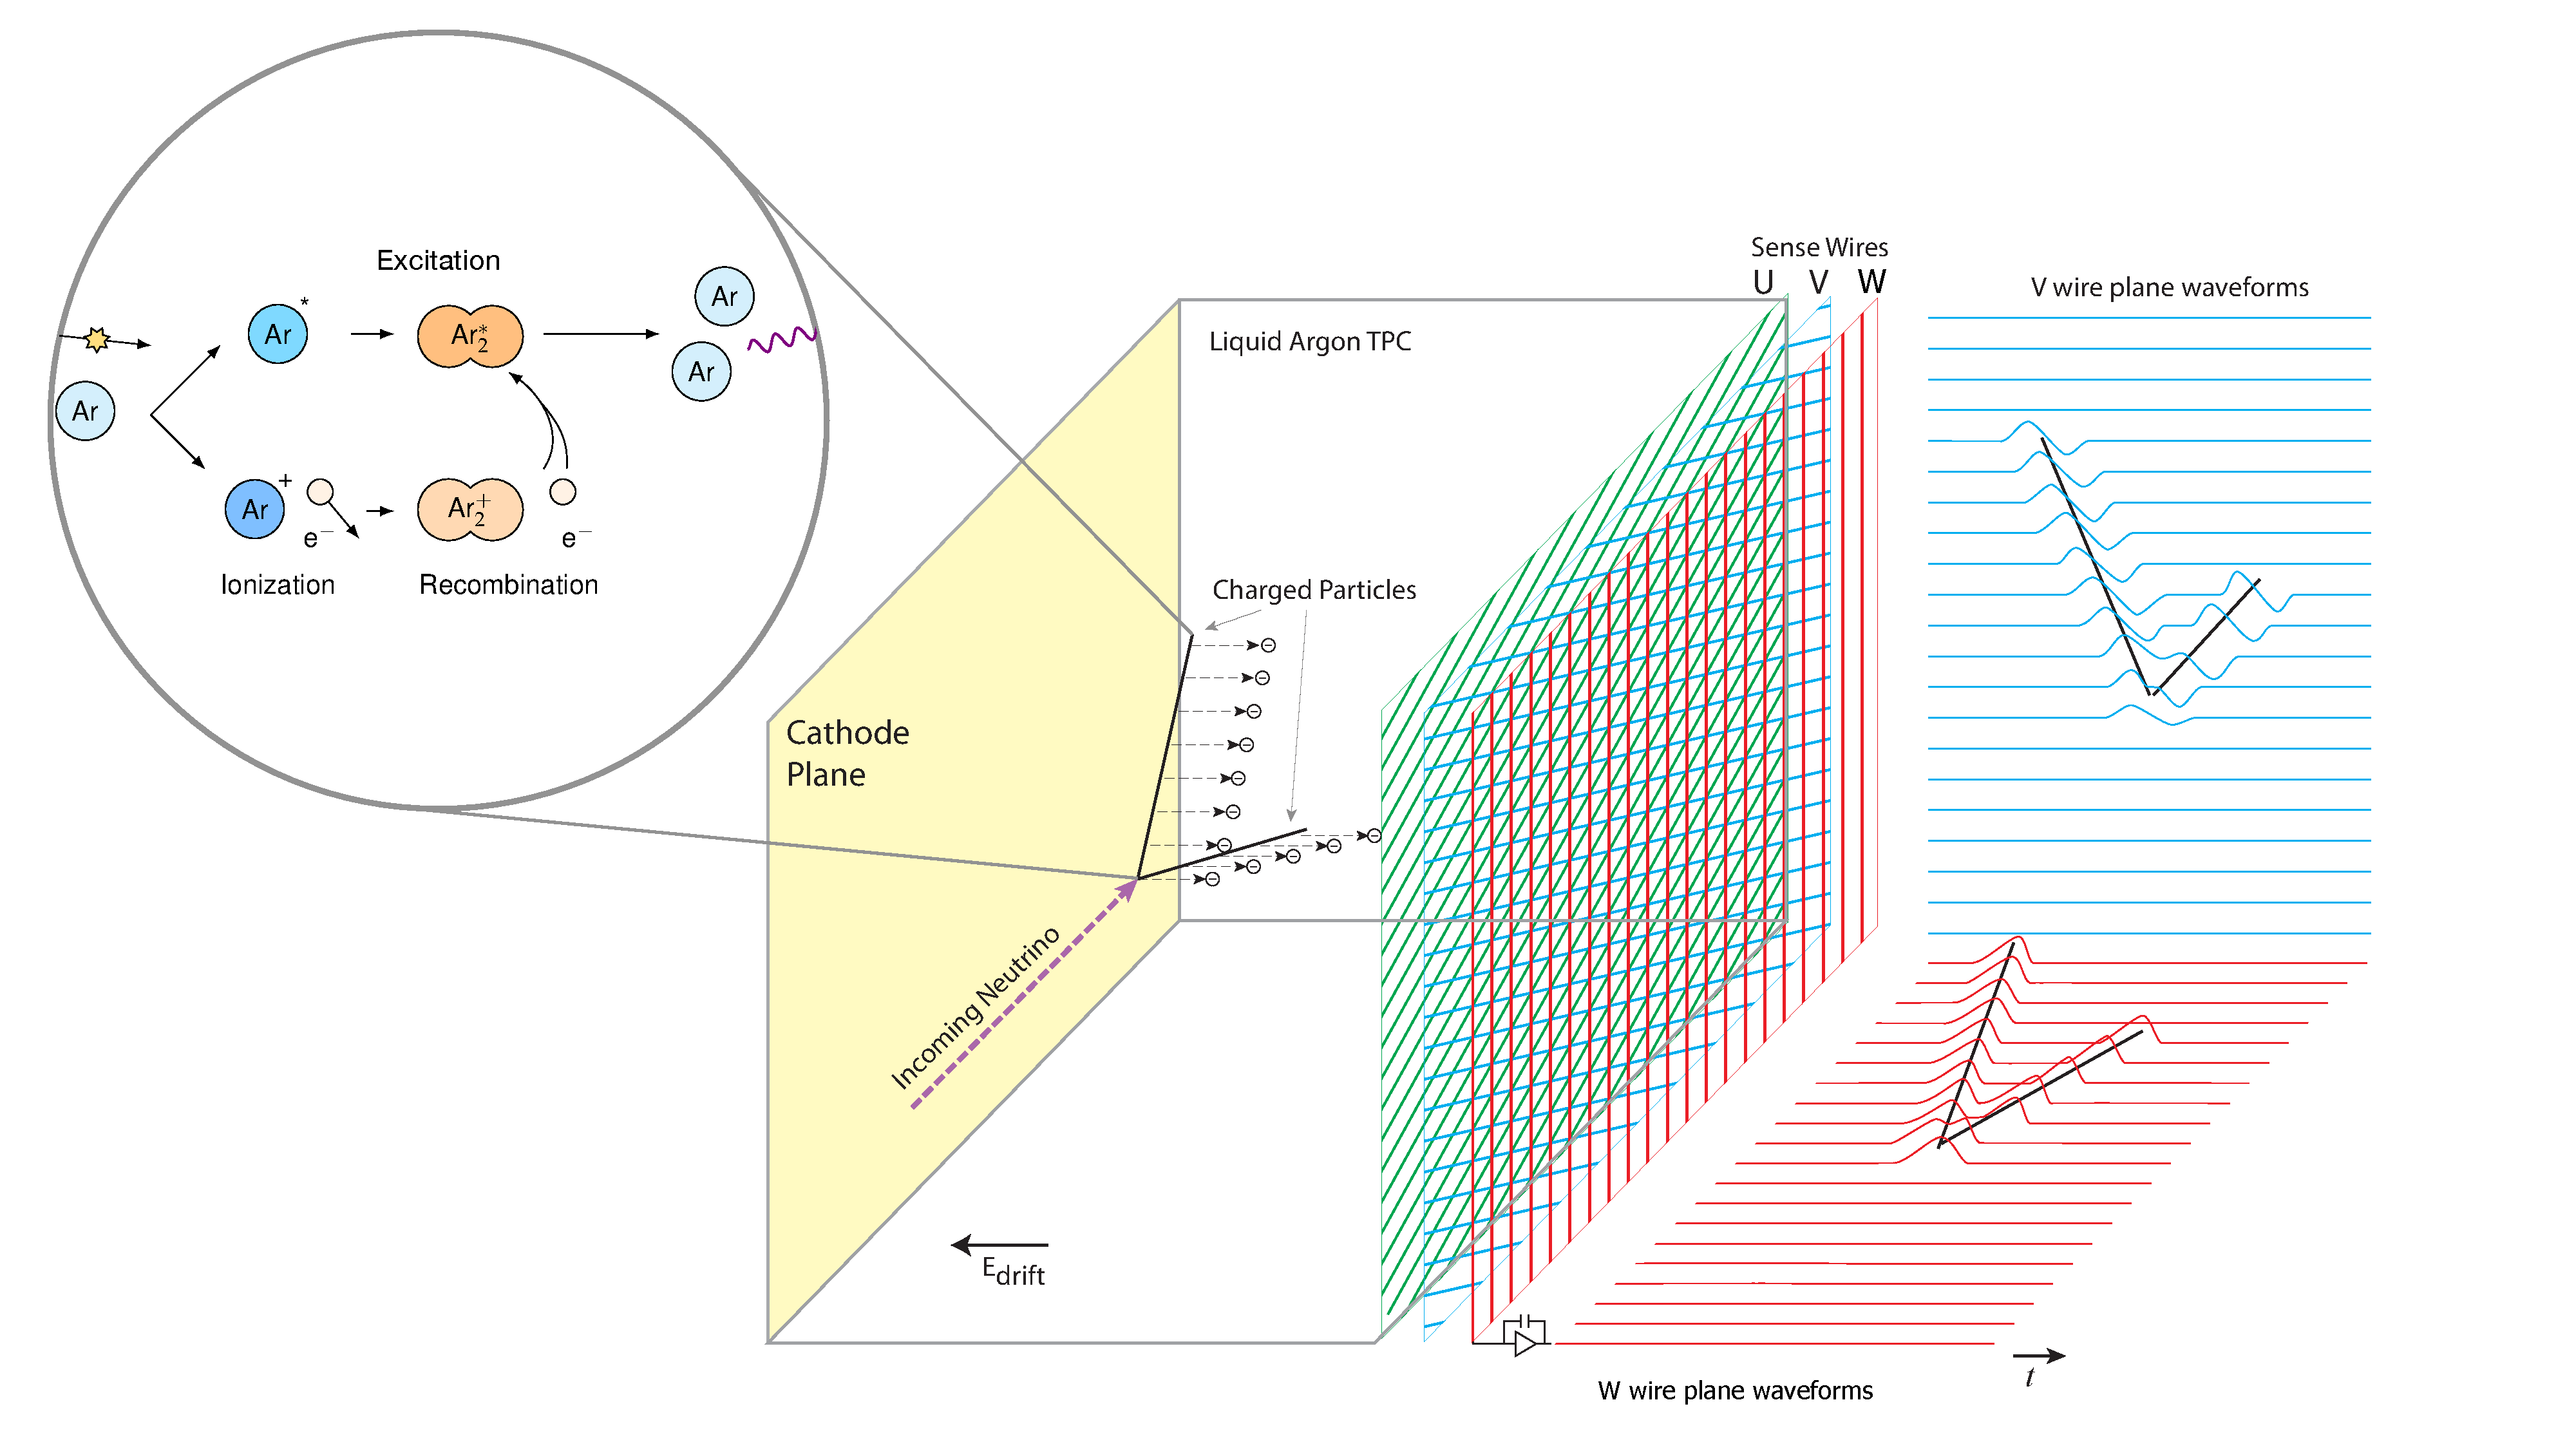
\includegraphics[width=\linewidth, trim={0 0 1.5cm 0}]{detector/TPC_argon.pdf}
    \caption[LArTPC illustration]{Illustration of the working principle of a LArTPC detector. Once neutrinos undergo weak interaction, they ionise the material, producing a large quantity of free electrons that are drifted towards the wire planes. Image adapted from \cite{triozziStudyTriggerSystem}. }
    \label{fig:TPC}
\end{figure}

The first TPCs were built primarily for high energy physics (HEP) applications, and many are still in use for major experiments, such as the ALICE tracker \cite{Lippmann:2014lay}. Carlo Rubbia proposed using liquid argon (LAr) as an interaction target for a TPC, thereby inventing the LArTPC concept for neutrino detection \cite{rubbiaLiquidArgonTime1977}. Liquid argon is an attractive material for particle detection, especially for neutrino physics, given its physical properties \begin{enumerate}
    \item LAr has a high density at \SI{1.39}{\gram\per\centi\meter\cubed} and a high atomic mass, which, combined with the small cross-section of $\PGn$-Ar interaction, allows for more probable detection than most gases.
    \item Being argon a noble gas, it does not attach free electrons, allowing for a longer drift lifetime.
    \item It has high electron mobility, $\mu\simeq \SI{320}{\centi\metre\squared\per\volt\per\second}$ for $E\simeq\SI{0.5}{\kilo\volt\per\centi\metre}$ and $T=\SI{87}{\kelvin}$, allowing for fast drift velocity $v=\mu E \simeq \SI{1.6}{\metre\per\milli\second}$.
    \item The LAr radiation length $X_0\simeq\SI{14}{\centi\metre}$ allows mm-scale calorimetry sampling of neutrino events while having a precise discrimination between electron- and photo-induced electromagnetic showers. Photons produced at the primary vertex usually show a greater conversion gap between the interaction and the starting points of the EM shower; additionally, photo-induced electromagnetic showers display an ionisation pattern in the first centimetres of the shower development compatible with two minimum ionising particles (MIP), whereas electron-induced showers show a pattern compatible with a single MIP.
    \item Ar is both easy and cheap to obtain. In Earth's atmosphere, it is the third most abundant gas, and can be liquified using nitrogen: this allows for great scalability required to use it for large-scale detectors.
    \item LAr boiling temperature of \SI{87.3}{\kelvin} causes most organic impurities to be frozen out to very low levels. This increases the drift electron lifetime. 
\end{enumerate}

Inside a LArTPC, once the neutrino undergoes weak interaction, it produces secondary charged ionising particles. These ionise LAr nuclei, creating $\mathrm{Ar^+},\ \Pem$ ionisation pairs and producing scintillation light. Roughly \SI{42}{\kilo e} are produced for each MeV of deposited energy\footnote{This number is dependent on the electric field strength inside the detector. This value is the reference with a nominal electric field of $\sim \SI{500}{\volt\per\centi\meter}$.}, which are then drifted by means of an electric field toward the anode plane assembly (APA). At the anode three planes of wires are placed in sequence, referred to as induction-1 (I-1), induction-2 (I-2) and collection (C) planes --- \autoref{fig:TPC} shows the common convention, which is to call the three planes $u$ (I-1), $v$ (I-2) and $w$ (C). The planes are properly voltage biased to achieve a nearly perfect transparency of the first two wire planes (I-1 and I-2) with respect to the drift electrons, enabling them to induce a charge on the first two planes and only be collected by the third plane. Given a nominal electric field inside the detector $E$, a good ``transparency'' of the successive wire planes to the drifting electrons is obtained by requiring that $E_2\geq F\times E_1$, and $E_1 \geq F \times E$ --- where $E_1$ and $E_2$ are respectively the field values in the I-1 to I-2 gap and I-2 to C gap --- with the scaling factor $F\in(1.2, 1.5)$. Due to the ionisation charge inducing a current on the first two planes and depositing the charge only on the third, the signal collected by the three sets of wires is intrinsically different: on the first two, the signal is bipolar, whereas on the third plane, the signal is unipolar. 

The three planes have their wires orientated at different angles to be able to  collect different ``projections'' of the same interaction happening inside the detector. Using this information, it is possible, in the reconstruction stage, to obtain a $\mathcal O(\si{mm^2})$-scale $(y,z)$ image of the interaction. The third $x$ coordinate is recovered using the timing information. In fact, when charged particles cross LAr, aside from creating ionisation pairs, they produce scintillation light, which constitutes a prompt signal used to assign the $t_0$ information. This way, the missing coordinate is reconstructed by comparing the time at which the electron is recorded on the wire with the prompt scintillation reference time $t_0$, and knowing the drift velocity of ionisation electrons inside LAr, $x = v_\mathrm{d}\times (t - t_0)$. 

Contributing to the formation of scintillation light within LAr are two processes, pictured in the inset of \autoref{fig:TPC} \begin{itemize}
    \item excitation of Ar followed by the formation of the excimer state $\mathrm{Ar_2^*}$, which decay with the production of scintillation photons, \begin{equation}
        \mathrm{Ar^* + Ar} \to \mathrm{Ar_2^*} \to \mathrm{2Ar}+\PGg;
    \end{equation}
    \item recombination of ionized argon atoms with a free electron, especially frequent with clouds of $\Pem$ around ionized $\mathrm{Ar^+}$ nuclei, \begin{equation}
        \mathrm{Ar^++Ar} \to \mathrm{Ar_2^+}\Pem \to \mathrm{Ar_2^*} \to \mathrm{2Ar}+\PGg;
    \end{equation}
\end{itemize}

These two processes combined produce \num{20000} monochromatic vacuum ultraviolet (VUV) photons per MeV of deposited energy, with a wavelength of $\lambda = \SI{128}{\nano\metre}$. This light presents two components, one so-called ``fast'', with a characteristic time $\tau\sim\SI{6}{\nano\second}$, and one ``slow'', $\tau\sim\SI{1.5}{\micro\second}$ components. Scintillation light is crucial, as already mentioned, for precise determination of the global timing required to reconstruct the missing coordinate in the 3-dimensional interaction from the 2-dimensional ``views''. Additionally, as I will briefly discuss later on, scintillation light is core for double-checking the $(y,z)$ positioning of the interaction, providing the so-called ``light barycenter''. 

It should be noted, however, that aside from all the mentioned great properties, there are some drawbacks to the use of LAr for particle detection. First and foremost, a complete understanding of the $\PGn$-Ar interaction has not been reached yet, so there are great systematic uncertainties related to the parametrisation of the interaction cross-section. Secondly, in order to keep argon in its liquid phase and minimise the organic impurities, a great effort is required for the design of the cryogenic infrastructure. 

Whilst this latter problem is intrinsic to the LArTPC design and requires ad hoc designs and implementations of the cryogenic infrastructure to be optimised, the former problem is addressed in the SBN programme by using two functionally identical LArTPC detectors, which allows the cancellation of many systematic uncertainties when performing a joint oscillation analysis. 

Finally, even though LAr was chosen for its large electron mobility, LArTPCs are intrinsically slow detectors, with drift times in the order of milliseconds. Hence, detectors operating at shallow depth, much like the two LArTPCs in the SBN programme, during the readout time window record significant cosmic activity. This reason led both the SBND and ICARUS collaborations to design the detectors to include an external cosmic ray tagger detector system (CRT) with nearly complete $4\pi$ coverage to veto most of the cosmic activity. 

\section{The SBN near detector: SBND} 

The Short Baseline Near Detector (SBND) is the near detector of the SBN programme at Fermilab. Located \SI{110}{\metre} from the proton-beryllium interaction target and containing \SI{112}{\tonne} of liquid argon, the SBND will provide precise flux measurements of unoscillated neutrinos for the far detector, ICARUS. As a ``flux monitor'', SBND will greatly reduce the impact of systematic uncertainties related to neutrino interactions in argon and the event reconstruction inside a LArTPC. Following nearly a decade of design, construction, and installation, SBND began operating in July 2024, commencing the collection of stable BNB data at an unprecedented rate of approximately \num{7000} neutrino events per day in December 2024 \cite{SBND:2025lha}. 

As for the ICARUS experiment, the physics goals of the SBND collaboration extend beyond the search for eV-scale sterile neutrinos; making use of its huge statistics, due to its proximity to the beam source point, SBND will allow for extremely precise $\PGn$-Ar interaction cross-section measurements in both the sub-GeV and GeV energy ranges. Additionally, the proximity to the neutrino source point allows the detector to cover both the on-axis as well as the off-axis phase space for BNB, expanding its capabilities to BSM physics studies like what is possible using NuMI for the ICARUS detector. 

SBND's LarTPC consists of a single module, with dimensions of $\qtyproduct[product-units = power]{5x4x4}{\meter}$, holding a total of \SI{112}{\tonne} of LAr. The structure contains two TPCs sharing two common cathode plane assemblies (CPAs) at the centre, parallel to the beam direction, and four anode plane assemblies (APAs) at the other two ends. The maximum drift length for the SBND detector is \SI{2}{\meter} which, for the nominal electric field of \SI{500}{\volt\per\cm}, leads to a maximum drift time of \SI{1.3}{\ms}. Each APA holds three planes of wires spaced \SI{3}{\mm} apart from each other, each hosting \num{2816} wires orientated at \SI{+-60}{\degree} (I-1/$u$ and I-2/$v$, respectively) and \SI{0}{\degree} with respect to the vertical $y$ axis. 

The photon detection system of SBND was developed to enhance the light collection and at the same time provide R\&D for future detectors. The first is addressed by making the cathode reflective and also coated in TPB, allowing the full scintillation light to be collected, while shifting the light from VUV to $\sim\SI{400}{\nm}$, making it detectable by PMTs. The second request for SBND's PDS was addressed by adopting two different light collection systems, PMTs, as for many other LArTPCs, and X-ARAPUCA. These are new innovative light collection technologies developed for the future detectors like protoDUNE and DUNE, adopting the silicon photomultiplier technology for light collection. 

The SBND detector finished its commissioning phase last summer and has since started collecting physics data alongside the ICARUS detector for use in the SBN programme. 

\section{The ICARUS-T600 detector}  \label{sec:ICARUS_T600}

The ICARUS (Imaging Cosmic And Rare Underground Signals) detector, the far detector for the SBN programme, with an active mass of \SI{476}{\tonne} of liquid argon, is the first ever large-scale operating LArTPC detector. It consists of two identical adjacent T300 modules with internal dimensions \qtyproduct[product-units = power]{3.6x3.9x19.6}{\meter}. Each T300 module houses two adjacent LArTPCs separated by a common cathode, with a maximum drift distance of $\simeq\SI{1.5}{\m}$, equivalent to a drift time of $\sim\SI{1}{\ms}$ for the nominal \SI{500}{\volt\per\cm} electric drift field.

The cathode is built up by an array of nine panels made of punched stainless steel, allowing for a \SI{58}{\percent} optical transparency between the two drift regions. The anode plane assemblies are made of three parallel wire planes, spaced \SI{3}{\mm} apart; each plane holds \SI{150}{\um} stainless steel wires orientated on each plane at different angles with respect to the horizontal direction. The wire orientation for the planes in the ICARUS detector is quite unique with respect to other operational LArTPCs. For both TPC in a T300 module, the Induction-1 wires are at \SI{0}{\degree}. The orientation of the  Induction-2 and Collection planes is different for the East and West TPC in each T300 module. \autoref{fig:i2_c_planes_wirepitch_detail} illustrate this difference. For the East APAs, Induction-2 is orientated at \SI{+60}{\degree} and Collection at \SI{-60}{\degree}, whereas for the West APAs, their orientation is reversed, with I-2 at \SI{-60}{\degree} and C at \SI{+60}{\degree}. With this design, as clearly illustrated in the images on both sides of \autoref{fig:i2_c_planes_wirepitch_detail}, electrons drifting from either TPC ``see'' the wires in both the I-2 and C planes as identically orientated \cite{amerioDesignConstructionTests2004c}. 

\begin{figure}
    \centering
    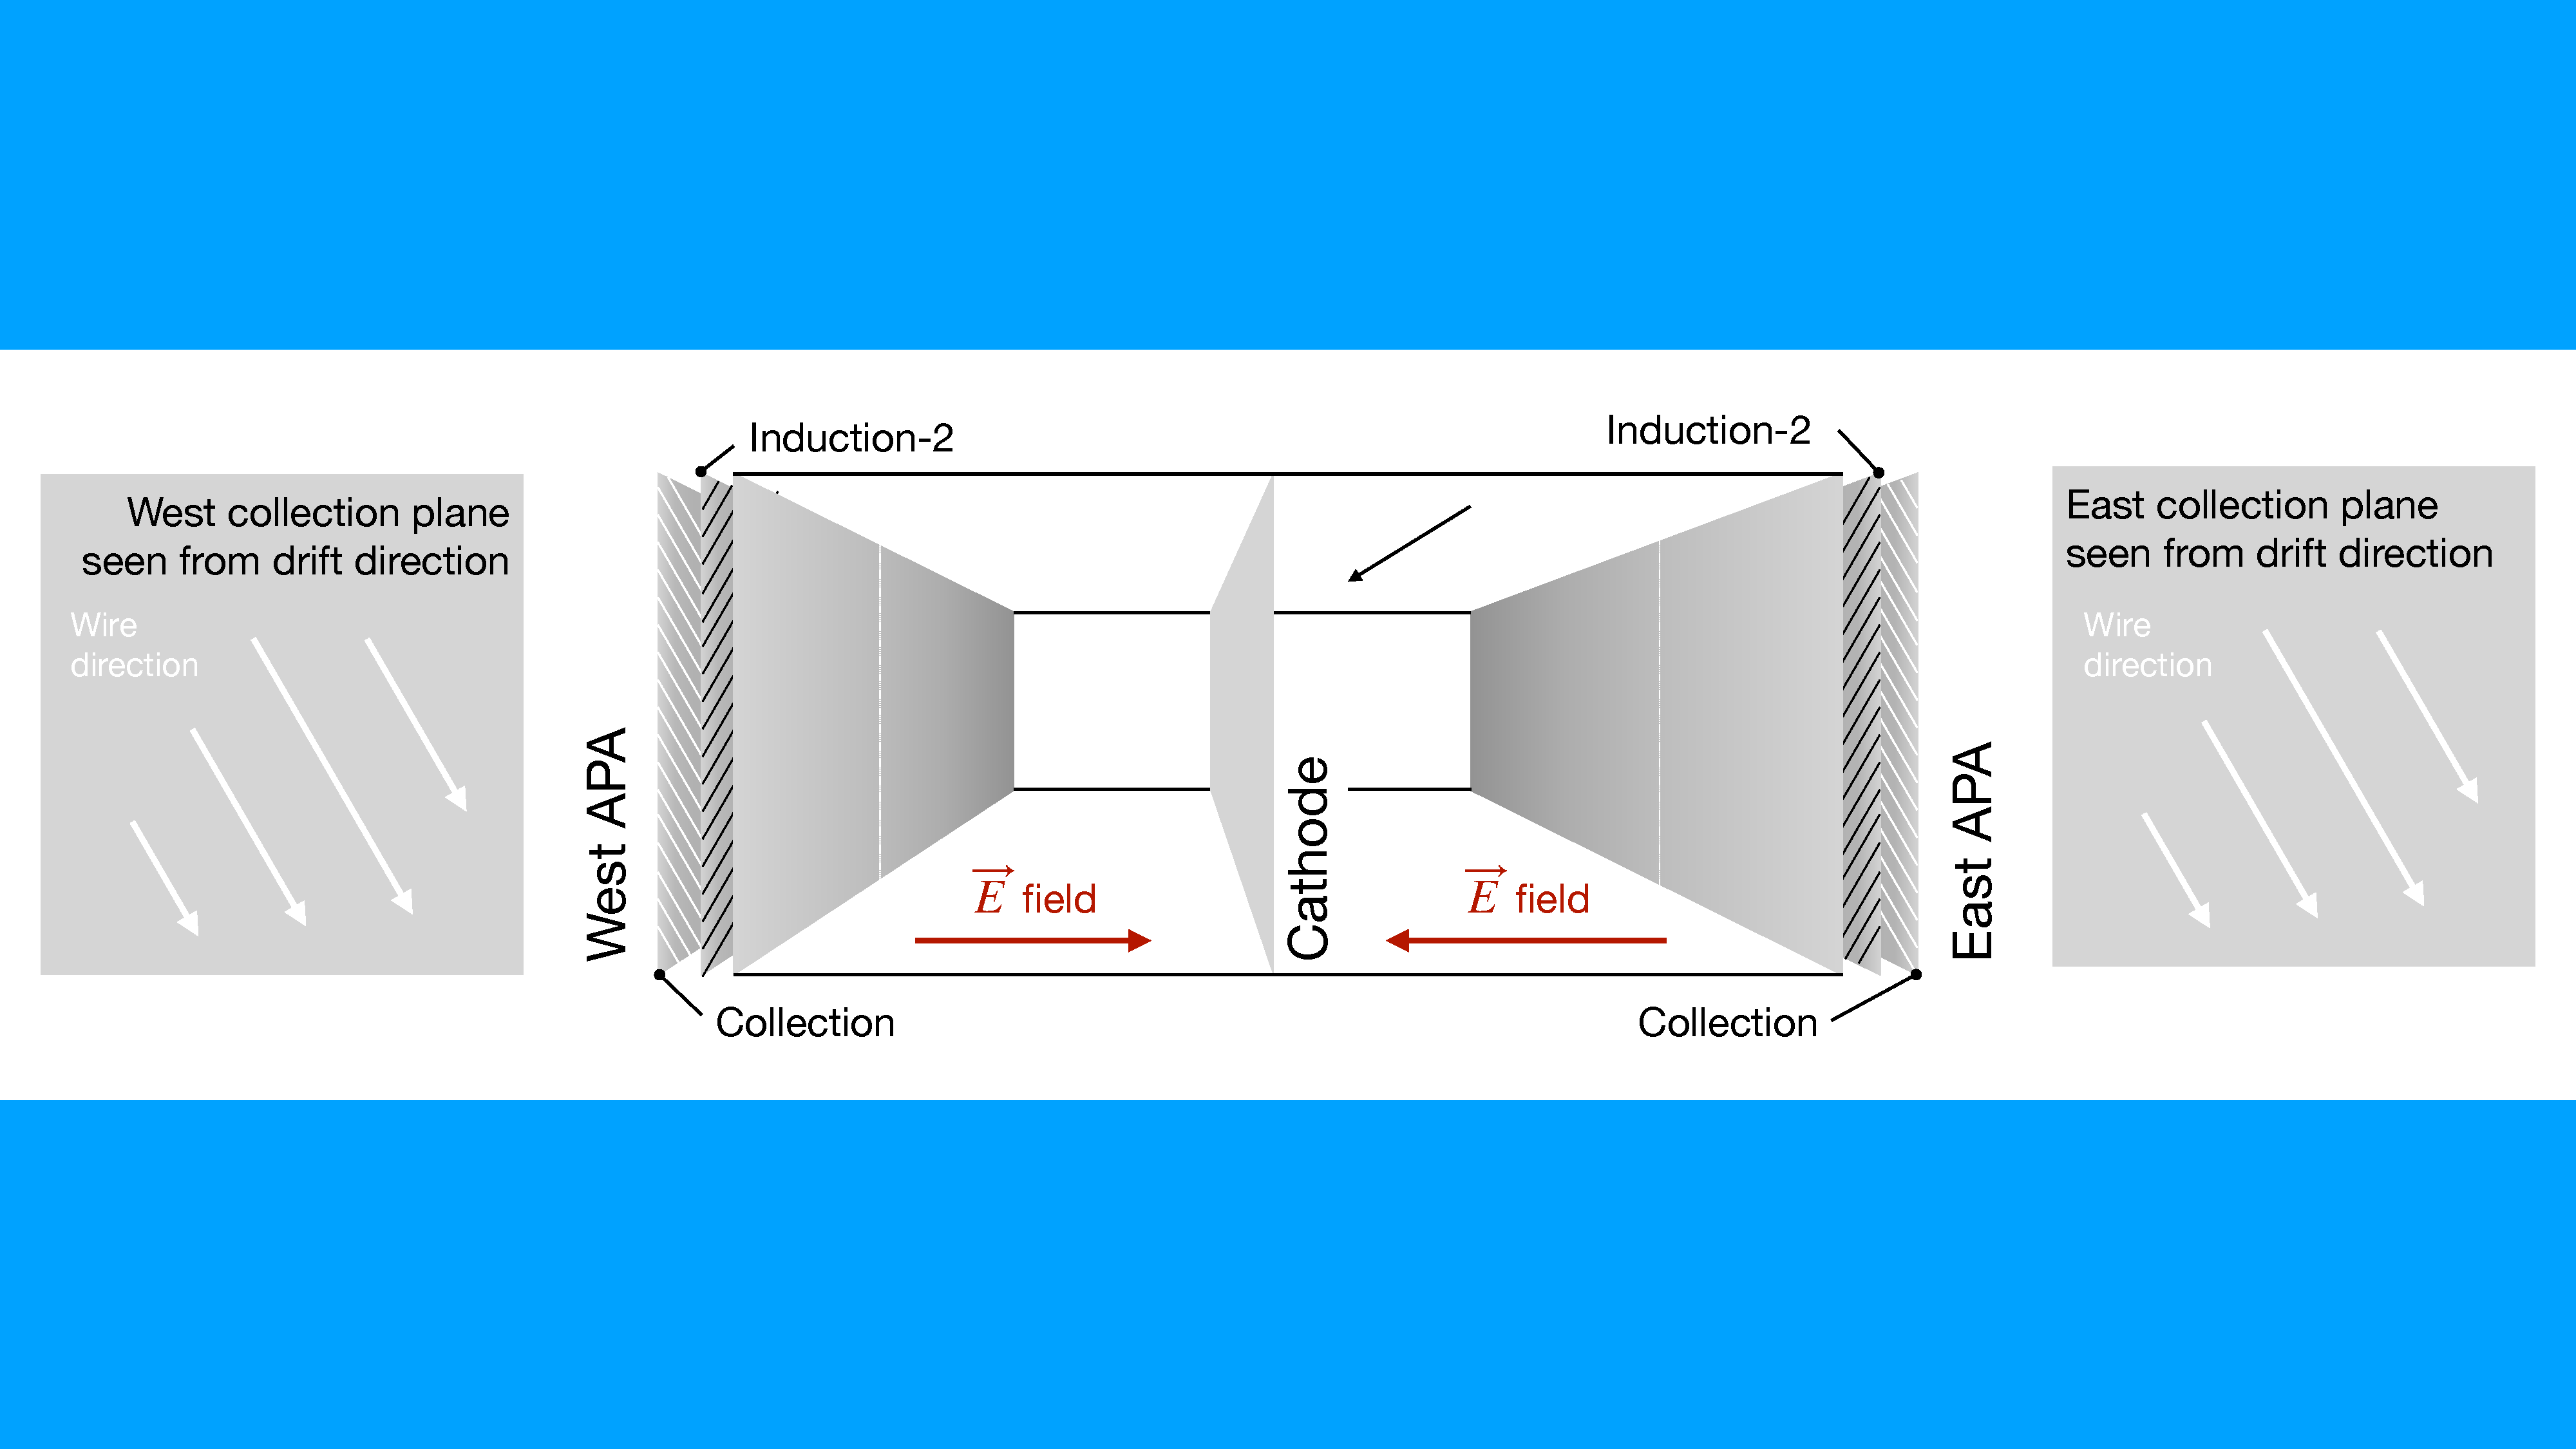
\includegraphics[width=\linewidth, trim={0 9.5cm 0 9.5cm}, clip]{detector/wire_orientation.pdf}
    \caption[T300 module Induction-2 and collection planes wire orientation]{Illustration of the wire direction for the I-2 and C planes for the East and West APA for each T300 module. The two side panels show the wire direction as seen by an observer located at the central cathode plane looking in the drift direction. }
    \label{fig:i2_c_planes_wirepitch_detail}
\end{figure}

In total \num{53248} wires spaced \SI{3}{\mm} apart with lengths up to \SI{9}{\m} across the three planes are installed inside the detector. By appropriately voltage biasing the first two planes (Induction-1 and Induction-2), a non-destructive charge measurement is provided, whereas the full ionisation charge gets collected by the Collection plane. The three planes are kept at $-\SI{250}{\volt}$ (I-1), $-\SI{30}{\volt}$ (I-2) and $+\SI{250}{\volt}$. The scintillation light is collected by a set of \num{360} PMTs located behind the wireplanes in the APAs. Photos of the installed planes of wires and PMT mounting are in \autoref{fig:ICARUS_photo}. 

\begin{figure}
    \centering
    \subfloat[]{\includegraphics[height=5.5cm]{detector/TPC_wires_texts.pdf}\label{fig:ICARUS_wires}}
    \hspace{1em}
    \subfloat[]{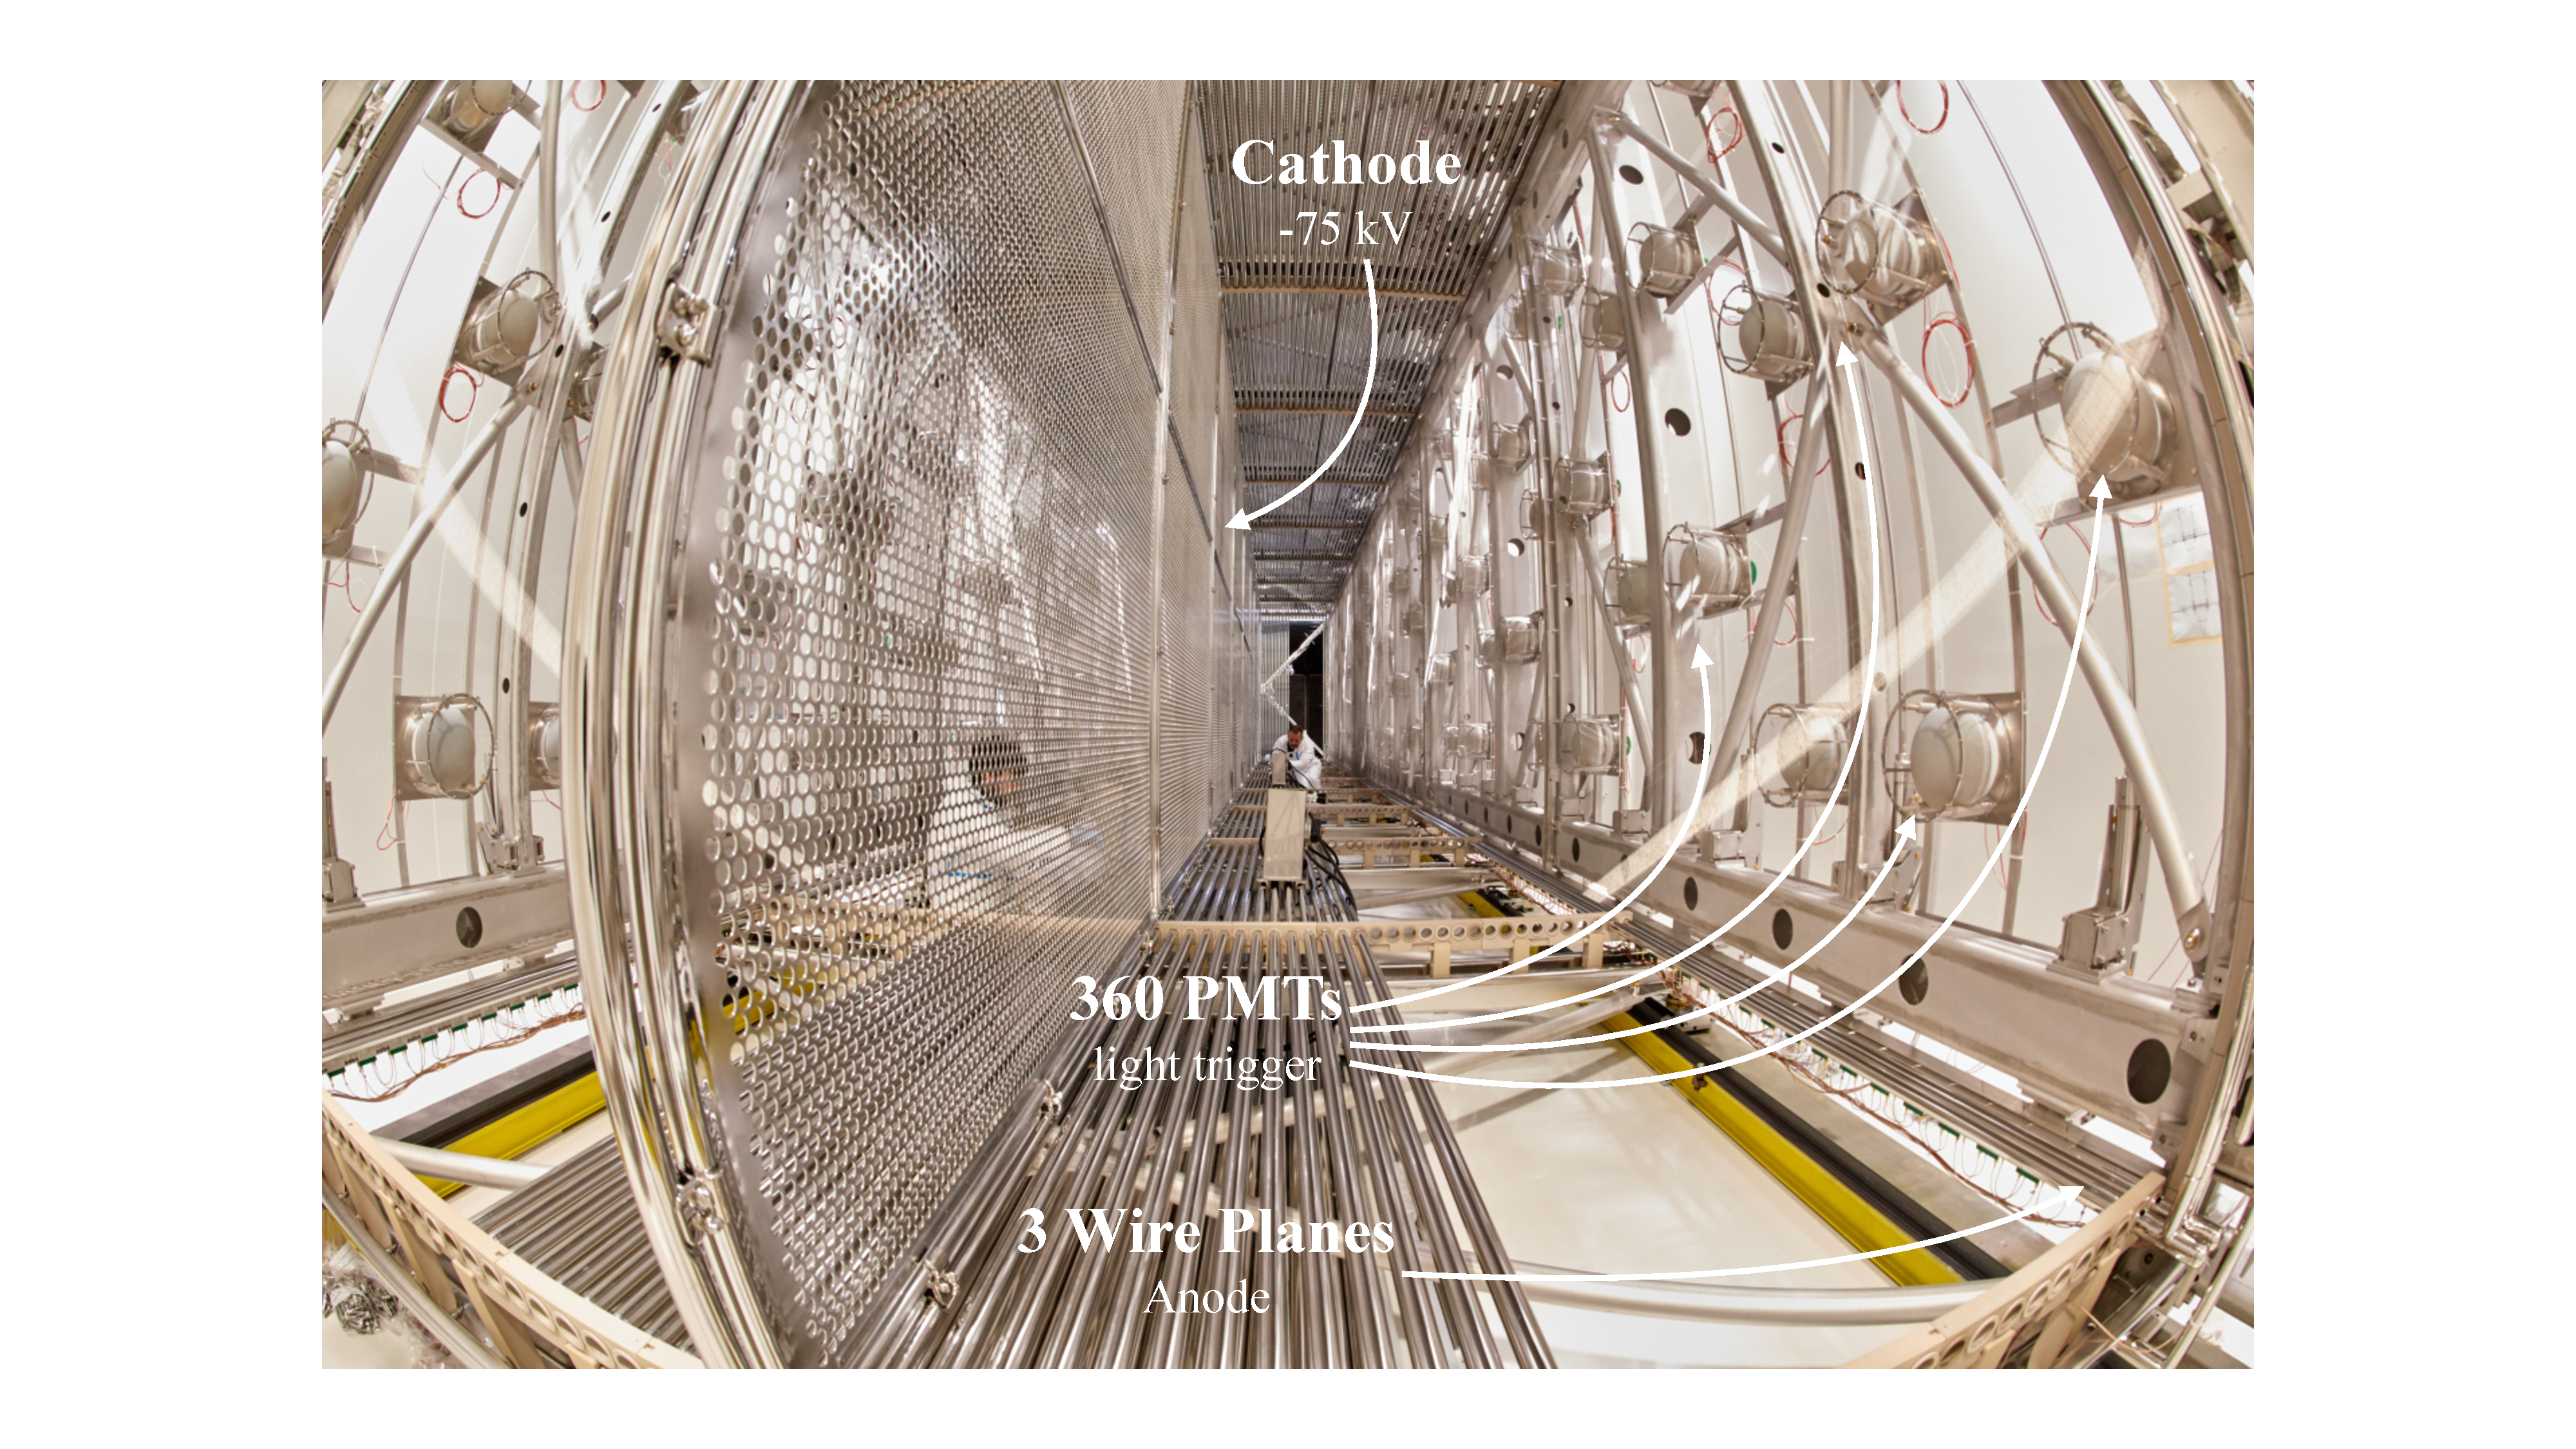
\includegraphics[height=5.5cm, trim={8cm 2cm 8cm 2cm}, clip]{detector/TPC_inner.pdf}\label{fig:ICARUS_PMTs_cage}}
    \caption[ICARUS TPC wires and field cage]{\ref{sub@fig:ICARUS_wires} shows the three planes of wires as installed in the ICARUS detector. \ref{sub@fig:ICARUS_PMTs_cage} shows one of the ICARUS TPCs's internals, with the common central cathode on the left and the anode plane assembly on the right, with the PMTs installed. Figures taken from \cite{amerioDesignConstructionTests2004c,abratenkoICARUSFermilabShortBaseline2023}. }
    \label{fig:ICARUS_photo} 
\end{figure}

The two T300 adjacent modules making up the ICARUS detector are housed inside a warm vessel, in which LN$_2$ is circulated, acting as a cold shield, preventing heat from external thermal insulation from reaching the LAr containers. The external warm vessel uses \SI{60}{\cm} of polyurethane foam to keep argon at its liquid phase just below the boiling point at \SI{87}{\kelvin}. The overall design of the ICARUS detector and the positioning of the two T300 modules are illustrated in \autoref{fig:ICARUS_scheme}. 

\begin{sidewaysfigure}
    \centering
    \begin{tikzpicture}
        \node at (0,0) {\includegraphics[width=\linewidth]{detector/SBN-FD_composite}};

        \draw[-*, white] (-1,2.5) node [left, white, fill=Gray!15!black] {TPC electronics} -- (0.5,2.25);
        \draw[-*, white] (-9,.5) node [right, white, fill=BrickRed] {Warm vessel} -- (-7.25,-1.5);
        \draw[-*, white] (4,2) node [right, white, fill=Plum!50!black] {Cryogenics} -- (3.25,3.5);
        \draw[-*, white] (7,-0.5) node [below, white, fill=Gray!15!black] {Top-CRT} -- (6.5,4);
        \draw[-*, white] (6,-1.75) node [right, white, fill=Gray!15!black] {Side-CRT} -- (5,-1);
        \draw[-*, white] (6,-3) node [above, white, fill=Gray!15!black] {Bottom-CRT} -- (3.5,-3.75);

        \draw[-*, white] (0,-4.5) node [below, white, fill=Gray!25!black] {East T300 cryostat} -- (-1,-3.5);
        \draw[-*, white] (-4.5,-4.5) node [left, white] {
            \begin{minipage}{4cm}
                \raggedleft
                TPC wireplanes + PMTs
            \end{minipage}} -- (-2.5,-2.5);

        \draw[-Latex, white] (-7,-3.5) -- (-7, -2.5) node[above] {$y$};
        \draw[-Latex, white] (-7,-3.5) -- (-6, -3.2) node[right] {$z$ (beam)};
        \draw[-Latex, white] (-7,-3.5) -- (-7.5, -3.35) node[left] {(drift) $x$};

        \draw[-*, black] (-4.5,5) node [left, black] {\SI{3}{m} concrete overburden} -- (-3,4.5);

        % \draw[step=1.0,white,thin] (-10,-5.5) grid (10,5.5);
        % \foreach \i in {-10,...,10} {
        %     \node [below] at (\i,-5.5) {$\i$};
        % }
        % \foreach \i in {-5,...,5} {
        %     \node [left] at (-10,\i) {$\i$};
        % }

        
    \end{tikzpicture}
    \caption[ICARUS detector illustration]{Illustration of the ICARUS T600 detector at Fermilab. Surrounding the warm vessel is the $4\pi$ coverage CRT. Above the warm vessel, the TPC readout warm electronics are placed, alongside the proximity cryogenics. Inside the warm vessel two identical (east and west) T300 modules are hosted, each containing two TPCs sharing a common cathode at the centre and two anode plane assemblies, one on each side.}
    \label{fig:ICARUS_scheme}
\end{sidewaysfigure}

The ICARUS collaboration successfully collected neutrino interactions during a three-year run at the deep underground laboratories beneath the Gran Sasso Mountains, LNGS (Laboratori Nazionali del Gran Sasso) from 2010 to 2013 \cite{amerioDesignConstructionTests2004c}. The nearly \num{3000} neutrinos collected by the ICARUS detector at LNGS were produced by the CERN to Gran Sasso Neutrinos beam (CNGS) with energy of \qtyrange{10}{30}{\GeV} using protons from the S$\Pp\PAp$S accelerator at CERN. 

The ICARUS detector operating at LNGS demonstrated the superior detection capabilities of the liquid argon TPC design: the detector showed a remarkable $\Pe/\PGg$ separation and particle identification exploiting the measurement of $\dv*{E}{x}$ versus range. The momentum of escaping muons has been measured by studying the multiple Coulomb scattering with $\sim\SI{15}{\percent}$ average resolution in the \qtyrange{0.4}{4}{\GeV} energy range. 

LNGS operations demonstrated the feasibility of archiving an exceptionally high level of LAr purity, with a $<\SI{50}{ppt}$ O$_2$-equivalent level of impurities. In 2013 the low-point record of \SI{20}{ppt} O$_2$-equivalent level of impurities was reached \cite{antonelloExperimentalObservationExtremely2014}, corresponding to an exceptionally high electron drift lifetime of \SI{16}{\ms}, marking a milestone for many future experiments, such as the Deep Underground Neutrino Experiment (DUNE). Furthermore, during this activity period, the ICARUS detector probed the sterile neutrino picture alongside the OPERA detector \cite{antonelloSearchAnomaliesNeappearance2013, antonelloConclusiveConsiderationsComparison2015, agafonovaNewResultsNm2013}, providing essential limits toward a better --- tough not definitive --- understanding of the short-baseline neutrino anomaly. 

From 2015 to 2017 the ICARUS detector underwent a thorough overhaul, first at Laboratori Nazionali di Legnano, Padova (Italy) and then at CERN in the Nutrino Platform framework (WA104/NP01 project), where the TPC electronics were updated to withstand the higher throughput a shallow-depth operation could require, as well as the light collection system. It was then moved in 2018 at Fermilab, where it was placed on the BNB baseline at a distance of \SI{600}{\m} from the source target, operating as the far detector for the SBN programme, collecting data from the Booster Neutrino Beam and from the NuMI beam. 

All the ICARUS subsystems --- TPC, PMT and CRT --- were commissioned from early 2021 to June 2022, when also the deployment of the concrete overburden was completed \cite{abratenkoICARUSFermilabShortBaseline2023}. This avoids heavy neutral particles entering the TPC volume, resulting in a less noisy event. 

After commissioning ended, the first physics data collection run started, lasting until the summer shutdown. Following Run-1, the ICARUS detector was able to collect three more physics runs until the recent summer shutdown. The collected/delivered efficiency is estimated to be greater than \SI{95}{\percent}, with a collected \SI{7.54e20}{POT} for BNB using the FHC mode and a total \SI{6.35e20}{POT} for the NuMI beam, split between \SI{3.53e20}{POT} in FHC mode and \SI{2.82e20}{POT} in RHC mode. \autoref{fig:BNB_NuMI_POTplot} shows the cumulative POT collected from the start of the ICARUS operations to this day. 

\begin{figure}
    \centering
    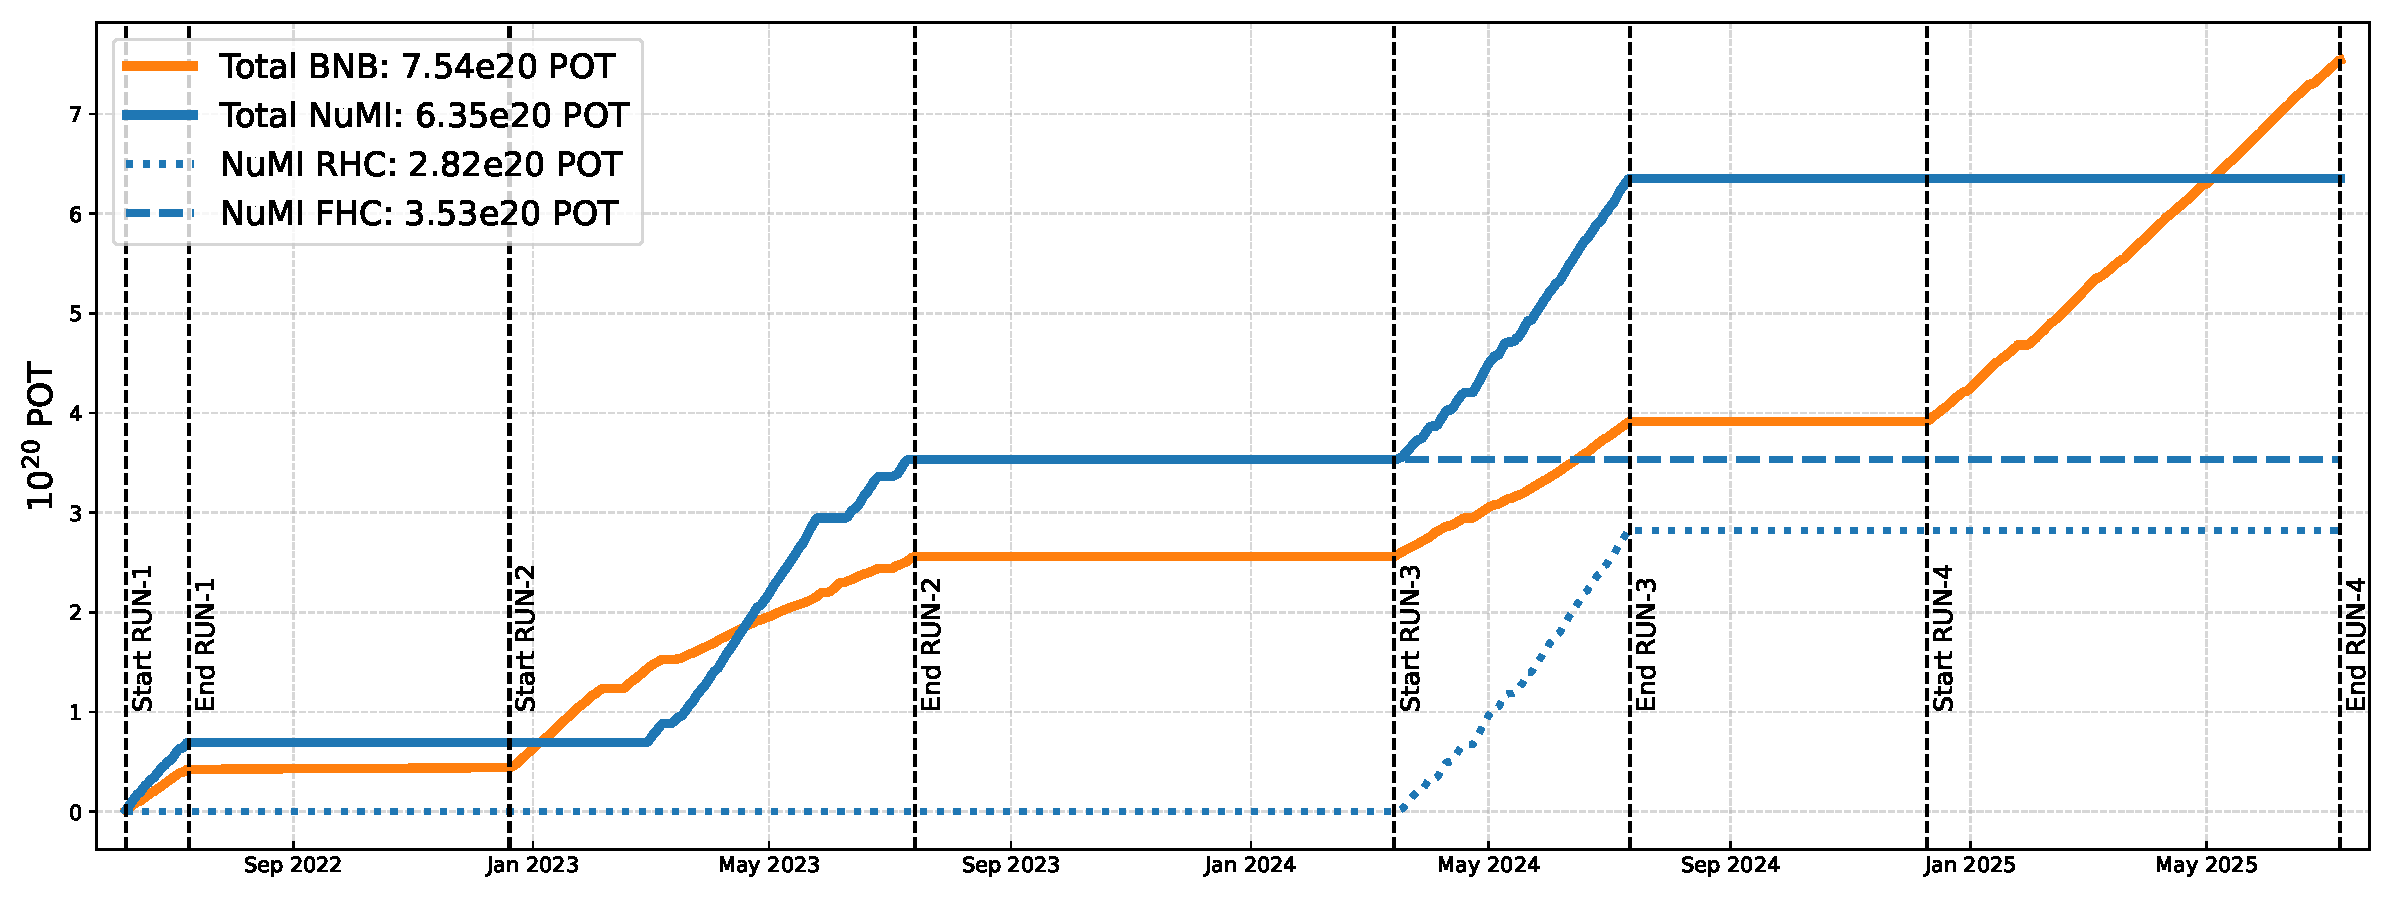
\includegraphics[width=\linewidth]{beams/cumulative_official_runs.pdf}
    \caption[BNB and NuMI collected POT]{Booster Neutrino Beam and NuMI beam collected proton-on-target neutrinos by the ICARUS detector. Courtesy of the run-coordination ICARUS group. }
    \label{fig:BNB_NuMI_POTplot}
\end{figure}

\subsection{The ICARUS subsystems} 

All three components (sub-detectors or sub-systems) of the ICARUS detector, upgraded during the detector overhauling process at CERN, are essential for the detector operation and to accomplish its physics goal.

\paragraph{TPC} One of the largest overhauls performed at CERN was the complete redesign of the TPC electronics \cite{bagbyOverhaulInstallationICARUST6002021}. During operation at LNGS, the wires were grouped in bunches of 576 wires, read out and filtered to achieve a unipolar signal from all planes. This was convenient in terms of post-processing but showed strong limitations in the case of intense showers. Such an approach would not have been compatible with the high rates foreseen for the ICARUS shallow-depth operations at FNAL. The new system maintains the previous architecture, which allows for a continuous triggerable  multi-buffered waveform recorder for each wire of the detector with a more advanced design. 

TPC wires are grouped together in bundles of 18 cables and feed through the 96 chimneys positioned above the TPC cryostats. At the other end of the chimneys, the signal is read by the front-end electronics, contained in custom-designed mini-crates mounted on the ultra-high vacuum feedthrough mounted on top of the chimneys. The interface between the TPC wires and the front-end electronics is given by the Decoupling and Biasing Boards (DBBs); each DBB is designed to house two isolated 32-channel banks, allowing each TPC wire to be biased at the proper voltage, enabling proper transparency to ionisation charges, and at the same time preventing parallel noise contributions to wire signal from leakage currents. DBBs are designed to operate in GAr (gaseous argon) and can provide a maximum of \SI{400}{\volt} of voltage bias. The \num{53248} TPC wires are bundled in \num{1664} 32-channel bunches and fed to \num{856} DBBs on the 96 chimneys: on each chimney flange are installed 9 DBBs, serving 576 TPC wires. It is important to note that, despite both MicroBooNE and SBND having the TPC readout electronic cold to allow for lower noise RMS, ICARUS has opted to keep its TPC electronic partially warm (outside of the TPC cryostat), allowing for easy serviceability. 

The analogue signal is then fed to custom-designed CAEN A2795 boards, housing eight amplifier boards, each capable of integrating and digitising eight channels, for a total of 64 channels for each CAEN board. High throughput is accomplished by employing optical fibre connections in a serial link with a bandwidth of \SI{1.25}{\giga b\per\second}. The digital signal is expressed in units of ADC counts, with the overall TPC electronic giving 1 ADC count per $\sim65\ \Pe$ (or equivalently, $\dv*{Q}{x}\simeq \SI{1000}{ADC\per\cm}$ for a MIP, for which $\dv*{E}{x}\simeq\SI{2.1}{\MeV\per\cm}$).

\paragraph{Light collection system} As mentioned before, once a charged ionising particle crosses liquid argon, ionising it, scintillation light, or VUV photons, is produced from the deexcitation of argon dimers. The light information is crucial for the operation of the ICARUS LArTPC, providing essential information to the event trigger, identifying the interaction occurring in the BNB and NuMI spill gates, as well as calorimetric and position information, useful to complement the 3D track reconstruction by providing absolute timing for each track. 

The ICARUS Light Detection System, or LDS, consists of \num{360} Hamamatsu 8'' R5912-MOD PMTs deployed behind the plane of wires (see figure \ref{fig:ICARUS_PMTs_cage}). Being the PMT glass opaque to the VUV \SI{128}{\nm} light produced by LAr scintillation, they need to be coated with a \SI{200}{\um\per\cm\squared} layer of tetraphenyl butadiene (commonly known as TPB) to convert the VUV light into visible light. 

All PMTs are mounted onto the TPC mechanical frames using a supporting system that allows the PMT to be positioned \SI{5}{\mm} behind the Collection plane. A stainless steel grid cage is mounted around each PMT to mitigate the induction of fake signals on the nearby wire planes by the relatively large PMT signals. The PMTs can be calibrated in time with a laser system based on a Hamamatsu PLP10 laser  diode, emitting laser pulses with $\lambda = \SI{405}{\nm}$ and an FWHM of \SI{60}{ps}, delivered to single PMTs via optical fibres. 

\paragraph{Cosmic ray tagger} Due to its installation at a very shallow depth at the Fermilab BNB baseline, the ICARUS detector is subject to a high rate of cosmic ray-induced interactions inside the detector volume. These particles are one of the primary background components of multiple neutrino physics analyses, as a muon inside the detector volume could be misidentified as a neutrino interaction. The Cosmic Ray Tagger (CRT) is therefore designed to address this very problem. It fully encloses the detector, covering it from all sides, tagging cosmic muons to clearly identify neutrino interactions. 

It is divided into three parts: the top, side and bottom modules. Each of these modules is, in its way, divided to allow for some granularity in the detector, employing the plastic scintillator technology. 

The top CRT is designed to cover the top part of the ICARUS detector; placed just below the \SI{3}{\m} concrete overburden, it intercepts almost \SI{80}{\percent} of the overall cosmic muon flux. It is comprised of 123 detector modules, each with an area of \qtyproduct{1.86x1.86}{\meter}. Each module is made of two orthogonal layers of 8 plastic scintillator bars in which the light is collected by wavelength-shifting optical fibres and read out on both sides by Hamamatsu silicon photomultipliers, enclosed in an aluminium box. The 32 SiPM signals of each Top-CRT module are connected to a CAEN DT5702 Front End  Board (FEB) to produce trigger logic based on  the coincidence between two SiPMs on the same bar and between two layers in a module. 

The side CRT is made using the recovered modules from the MINOS experiment, refurbished with the addition of the SiPM technology to read out the scintillation light.

Finally, the bottom CRT, placed under the detector, is made of 14 modules. Each module, coming from the Double Chooz experiment, is made of polystyrene strips, and the scintillation light is read out by Hamamatsu PMTs. 

In both side and bottom CRTs the scintillation light is collected by wavelength-shifter optical fibres that are read out, either on both ends or on one end, by light-sensitive detectors.  

% !TEX root=../main.tex

\chapter{ICARUS data processing and event reconstruction}
\label{chap:event_reconstruction}

% The ICARUS detector, described in \autoref{sec:ICARUS_T600} is a complex system, and a precise operation is required to make the most out of all its subcomponents. Each part of the online operation is essential and preliminary to the offline operations, consisting of the wireplane signal processing, the reconstruction of all the signals coming from the different subsystems and their combination to obtain a final physics result. 



\section{Data acquisition} \label{sec:DAQ}


\paragraph{ICARUS trigger} In a few words, the ICARUS trigger employs the coincidence between the signal from the beam (BNB and NuMI) spill gates and the scintillation light to provide a global signal that activates  the acquisition windows for the TPC and PMT subsystems \cite{ICARUS:2025kai}. For TPC, the choice of the acquisition window is driven by the distance between the cathode and the anode. This is the maximum drift distance an ionisation electron produced in-time (during the beam spill gate, triggering the event) can travel. With a nominal electric drift field of \SI{500}{\volt\per\cm}, and a half-width of $\sim\SI{1.5}{\m}$, the maximum drift time is $\SI{1.6}{\ms}$. The acquisition window for PMTs is driven by the mean lifetime of LAr excited states. De-excitation of LAr produces scintillation light in two components, one fast $\tau\simeq \SI{6}{\ns}$ and one slow $\tau\simeq\SI{1.6}{\us}$ \cite{Segreto:2020qks}. To collect the entire scintillation light signal, the time window has to be thus greater than the BNB (NuMI) beam gate \SI{2.2}{\us} (\SI{10.1}{\us}). PMT sgnal is read in primitives of \SI{10}{\us}, with \SI{3}{\us} (\SI{7}{\us}) of pre-(post-)tigger buffer.  Additionally, in the case of a second light trigger in the \SI{10}{\us} immediate subsequent window the readout is extended by \SI{7}{\us}. In the case a global trigger is issued, three primitives are recorded, without the first pre-trigger buffer, so a \SI{26}{\us} window is readout \cite{ICARUS:2025kai}. 

The ICARUS trigger architecture allows for multiple configurations, i.e. the acquisition of different types of events \cite{ICARUS:2025kai}. The main ICARUS trigger physics configuration (on-beam majority) is based on the multiplicity of PMT signals in coincidence with the beam ``open'' spill gate. This configuration maximise the probability of collecting neutrino interactions and reduce the rate of cosmic triggered events. To perform detector calibration is however useful to have few runs with collected cosmic interactions. To archive this, Minimum bias configuration are created, bypassing the need of scintillation light signal to perform a global trigger, instead capturing the whole detector at the maximum rate possible with the DAQ capabilities, around \SI{4}{\hertz}. Additionally any mentioned global trigger configuration can be issued on- and off-beam, by adjusting a delay. The on-beam configuration has no delay with respect to the configuration, whereas the off-beam trigger has a delay of \SI{+33}{\ms}. 

\paragraph{Collection of the triggered events. } Once a global trigger is issued, the data acquisition system (DAQ), which communicates via TCP/IP protocol with the trigger system \cite{ICARUS:2025kai}, activates the readout of the whole detector, opening \SI{1.6}{\ms} and \SI{26}{\us} acquisition windows for the TPC and PMTs, respectively. ICARUS DAQ system is based on the \emph{artdaq} data acquisition software development kit (SDK) developed and maintained at Fermilab for use in several accelerator-based experiments \cite{Biery:2013cda}.  

% in the \emph{artdaq} language, and configurable applications for performing event-building (i.e. merging together the collected data fragments from each \emph{BordReader}, performed by objects inherited from \emph{EventBuilder} instances), data-logging and data-dispatch to downstream online data quality monitoring processes. 

The \emph{artdaq} SDK provides  customisable applications for reading data fragments (buffered piece of data form each of the ICARUS subdetectors modules) from detector elements identified as \emph{BoardReader} objects. Each BoardReader acquire the data stream for a part of one of the ICARUS subdetectors: TPC, PMT and CRT readout electronics, and from trigger and White Rabbit. 
The White Rabbit is one very important piece of hardware for the ICARUS detector, allowing precise (sub-nanosecond) scale timeing across the multiple subsystems using a network interface. 
Event counters and timestamps are assigned accordingly to each data fragment, which are then queued for data transfer. 
When a global trigger is issued, the trigger BoardReader stream is passed to the \emph{EventBuilder}, which are computers aimed at collecting the buffers from all the ICARUS subsystems and compacting them into a single event. Once the EventBuilder reads a trigger signal it also colect the streams from the other BoradReaders.  \autoref{fig:DAQ} shows a simplified illustration of the flow of the data signals from the ICARUS components to the creation of the full event. Once the events are created by the EventBuilder, they are distributed for monitoring the data quality and for long term storage. 

\begin{figure}
    \centering
    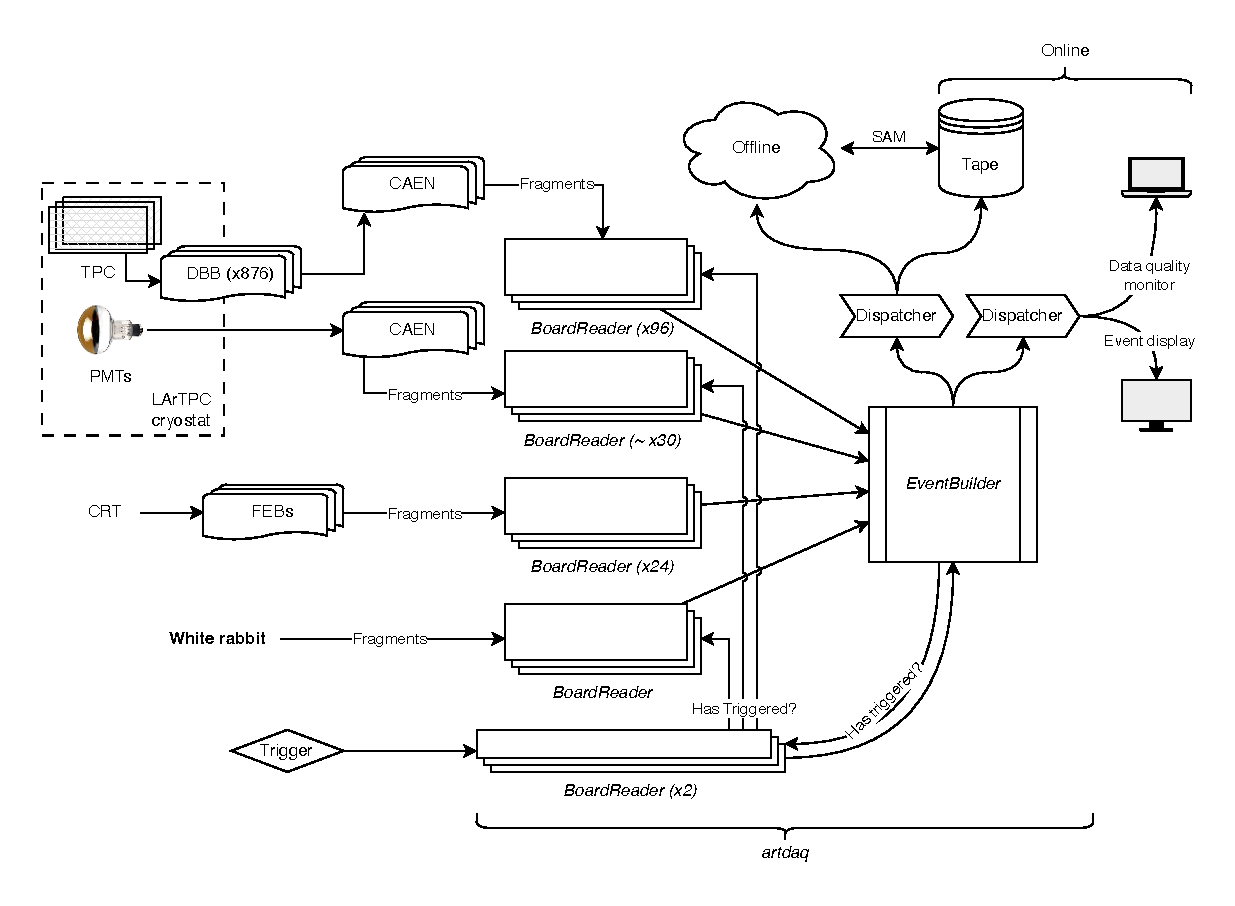
\includegraphics[width=\linewidth]{detector/DAQ_simplified.pdf}
    \caption[ICARUS DAQ illustration]{Simplified illustration of the ICARUS DAQ system. Further information is found in \autoref{sec:DAQ}. The number of parallel \emph{EventBuilder} instances could be defined $\geq1$, to allow for faster processing.}
    \label{fig:DAQ}
\end{figure}

\paragraph{TPC data} The TPC data input to the DAQ EventBuilder corresponds to the digitised waveforms from each TPC readout channel, representing the charge signal (as a function of time) induced by the motion of ionisation electrons drifted by the electric field inside the detector. 

\paragraph{PMT data} Similarly to the TPC data, the data from the PMTs correspond to the digitised waveforms of the readout of every PMT inside the detector. For any event triggered in coincidence with the beam spill, the digitised signals of all 360 PMTs are recorded in \SI{26}{\us} long time intervals, sampled at \SI{500}{\mega\hertz}. In addition to this data, whenever an off-time cosmic ray event crosses the volume, triggering scintillation light acquired by the PMTs in the \SI{+-1}{\ms} around the beam gate, all 180 PMTs belonging to the T300 module containing the interaction are recorded in \SI{10}{\us} long time intervals. 

\paragraph{CRT data} For the CRT system the DAQ acquisition and processing is slightly different \cite{ICARUS:2025rdw,Poppi:2023zmp,Poppi:2022vhg}. The ICARUS CRT components operate in self-trigger mode \cite{arteroponsStudyReconstructionNuMuCC, ICARUS:2025rdw}, whenever a CRT SiPM exceeds the threshold, the data from all 32 SiPM channels for each FEB is stored in internal buffers, holding up to \qtyrange{40}{80}{\ms} depending on which CRT sub-part is considered. The data from the top, bottom and side CRTs, which is a count as a function of time of photons readout by the SiPM at the ends of the scintillating strips, is aggregated within \SI{10}{\us} data fragments in the BoardReaders instances; once the global trigger is activated, \SI{+-25}{\ms} of CRT data fragments are sent from the BoardReader to the EventBuilder instance. 

\paragraph{Saved data} Downstream of the DAQ interface, events are written using the \emph{art} event-processing framework \cite{greenArtFramework2012} also developed at Fermilab, on which the \emph{artdaq} SDK is built. This allows interoperability between the DAQ interface and the offline analysis, without the need to convert the events saved from the DAQ interface into a format compatible with the high-level offline analysis. \emph{art} files are essentially ROOT files \cite{rene_brun_2019_3895860} with custom data types stored in them. The data collected by the ICARUS DAQ system are written in different file streams based on their specific acquisition mode, including the beam source (if on-beam), the specific trigger configuration active and its specific setting.

After a period of intense tests and validation of the system, the DAQ system allowed stable acquisition of high data rates up to \SI{5}{\hertz}. This is, however, larger than the amount of data input foreseen for the system with both BNB and NuMI beams and with the majority-based trigger configuration: the data throughput corresponds to ${\sim}\SI{1}{\hertz}$.

% In order to handle the large volumes of data stored on tape, the Fermilab-based SAM (serial access to metadata) system is exploited. This system associates a set of metadata information with each data file using Python scripts. This metadata is useful in offline analysis to create large datasets of files, identifying whether the files contain raw or processed data, run configuration, run number and so on.

% \section{ICARUS data processing}

% The output data files contain the aggregated data coming from all the \emph{BoardReader} instances in an event. For the TPC,  For the CRT system the DAQ acquisition and processing is slightly different \cite{ICARUS:2025rdw,Poppi:2023zmp,Poppi:2022vhg}. The ICARUS CRT components operate in self-trigger mode \cite{arteroponsStudyReconstructionNuMuCC, ICARUS:2025rdw}, whenever a CRT SiPM exceeds the threshold, the data from all 32 SiPM channels for each FEB is stored in internal buffers, holding up to \qtyrange{40}{80}{\ms} depending on which CRT sub-part is considered. The data from the top, bottom and side CRTs, which is a count as a function of time of photons readout by the SiPM at the ends of the scintillating strips, is aggregated within \SI{10}{\us} data fragments in the \emph{BoardReader}s instances; once the global trigger is activated, \SI{+-25}{\ms} of CRT data fragments are sent from the \emph{BoardReader} to the \emph{EventBuilder} instance. 

\section{ICARUS Data processing}

The output of all ICARUS sub-detectors is common across LArTPC detectors, which might have different TPC geometry and light collection configurations but share the same underlying technology. The \emph{art}-based \emph{LArSoft} framework \cite{Church:2013hea,Snider:2017wjd,Pordes:2017BL} is the common software development kit providing software infrastructure and algorithms for processing the collected data, and additionally providing tools that enable the simulation of the physics events and the detectors response, as well as the downstream event reconstruction. 

LArSoft allows to process the data by applying different algorithm, called modules, to the data stored in the \emph{art}/ROOT files. The modules are steered by configuration files that allow a great degree of flexibility. 
% The key to \emph{LArSoft} is the use of real-time configuration files that employ the \emph{Fermilab Hierarchical Configuration Language}, or \emph{FHiCL}, which specify how different modules of the processing chain should be run. 

The data processing and event reconstruction proceeds in two steps. First the raw data collected by the ICARUS DAQ is processed to produce a simpler representation of the signal, so from the raw digitized waveforms, \emph{hits} objects are created. Hits are objects containing the same information as the raw waveform, but in a more manegeable format. Inside this step, the signal on the wires, the signal from the PMTs and from the CRTs is analysed and translated into different hit types, depending on the subsystem. This step is commonly referred to as \emph{Stage0}. Once the data is processed, a second stage, referred to as \emph{Stage1}, aims at building a complete picture of the physics interaction happening inside the detector. This encompass, for example, the creation of the reconstructed interaction and its indetification from the hits reconstructed from the TPC wires. 

% When an event is saved from DAQ to data files and stored to tape, it is then available to be processed. The ICARUS data processing chain is split, like for many other LArTPC detectors, into two \emph{stages}, usually named \emph{Stage0} or \emph{reco1} and \emph{Stage1} or \emph{reco2}. Processing the raw collected data is a mandatory step in order for it to be properly analysed. 

% In the \emph{Stage0/reco1} step, all data  from the three sub-detectors is processed to produce a ``simpler'' description of the raw signal. This means to decode the raw signal and translate it into objects in the \emph{LArSoft} format for offline reconstruction. It also performs signal processing of the waveforms to identify physical signals, hits, that can then be used as input to the higher-level event reconstruction tools implemented in the \emph{Stage1/reco2} steps. 

\begin{figure}
    \centering
    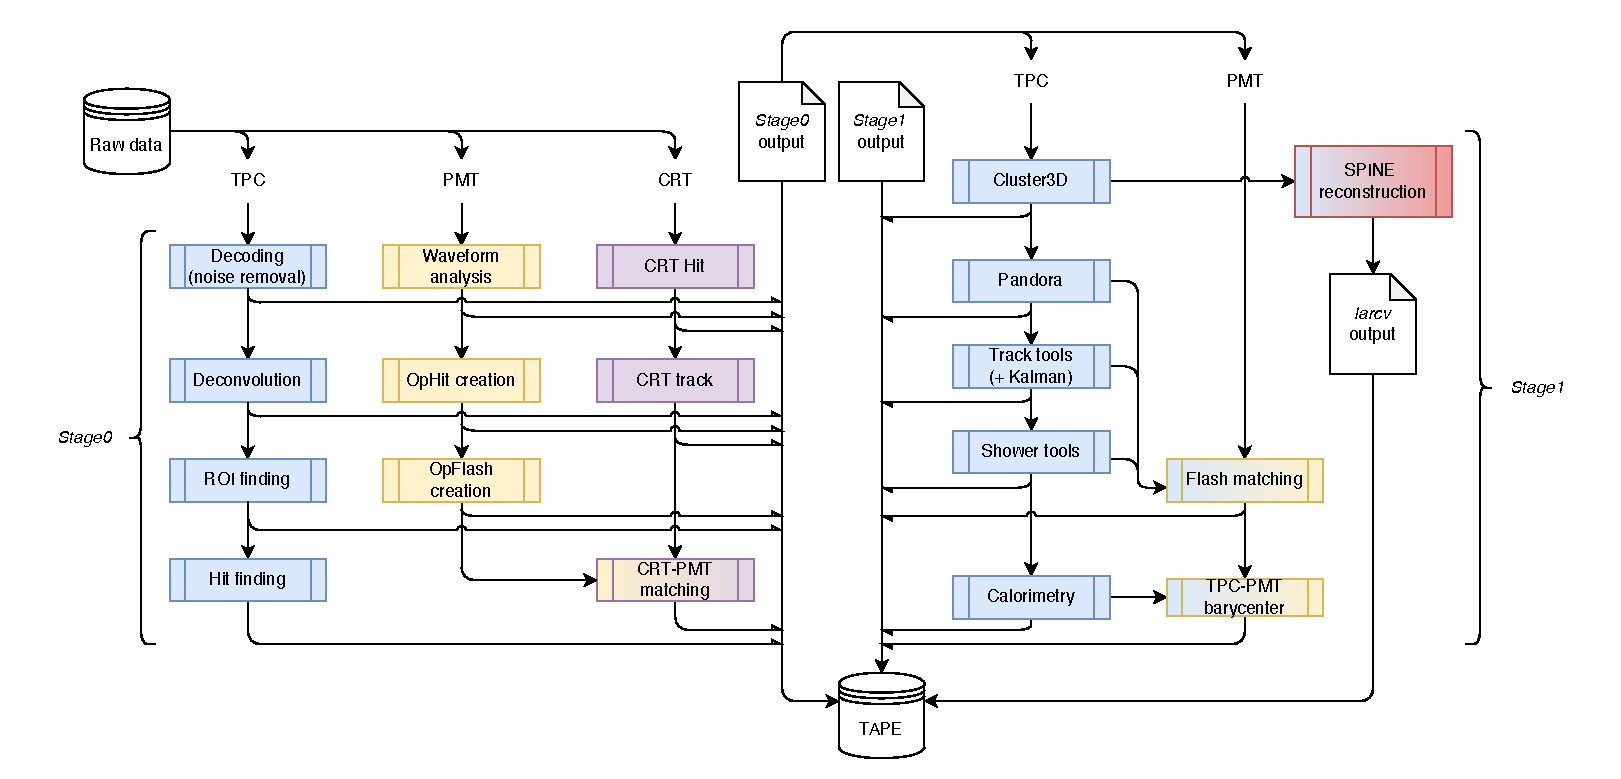
\includegraphics[width=\linewidth]{detector/data_processing_pipeline.pdf}
    \caption[\emph{Stage0} and \emph{Stage1} data processing pipeline]{Illustration of the data processing pipeline used in the ICARUS detector showing the steps involved in both \emph{Stage0} and \emph{Stage1}. }
    \label{fig:reco_stages}
\end{figure}

\autoref{fig:reco_stages} pictures the overall \emph{Stage0/Stage1} chain which is applied to the data files produced by the ICARUS DAQ. A detailed description of these steps follows in the next paragraphs. 

\subsection{Light reconstruction}

One of the first steps in \emph{Stage0} reconstruction addresses the reconstruction of the light signal. Reconstruction of the light signal associated with the event of interest is based on the recorded PMT signals in the events.

Light reconstruction starts from the identification of the PMT signal, using a threshold-based approach. To do so, a ``pedestal'' is defined, step which is performed using a sliding window, and mediating the photo electron counts to define the central value. The pedestal is subtracted from the raw signal, and the pedestal-subtracted waveform is used to identify the signal over the threshold, using three thresholds defining the start, tail and end time points of the PMT hit, called \emph{OpHit}. Once the three time values are identified, to OpHit is created. In a OpHit the start, end and tail timestamps are saved, and the area under the curve between these three points is computed. The integral of the waveform is proportional to the integral collected charge of the PMT that is protortional to the the collected light. If a start threshold is reached before the end of a previoud \emph{OpHit} the hit is truncated. \autoref{fig:PMT_reco}(a) shows the example of a PMT with a clear single \emph{OpHit}. 

After individual optical hits are reconstructed, they are clustered together into higher-level objects, called \emph{OpFlashes}, corresponding to multiple optical hits happening in proximity inside the detector, likely belonging to the same physical event inside the volume. \autoref{fig:PMT_reco}(b) shows the signal from multiple PMTs whose \emph{OpHit} will be clustered into a single \emph{OpFlash}.

All data products created in the \emph{Stage0} PMT processing are saved using the same \emph{LArSoft}-based structure to ROOT files. 

\begin{figure}
    \centering
    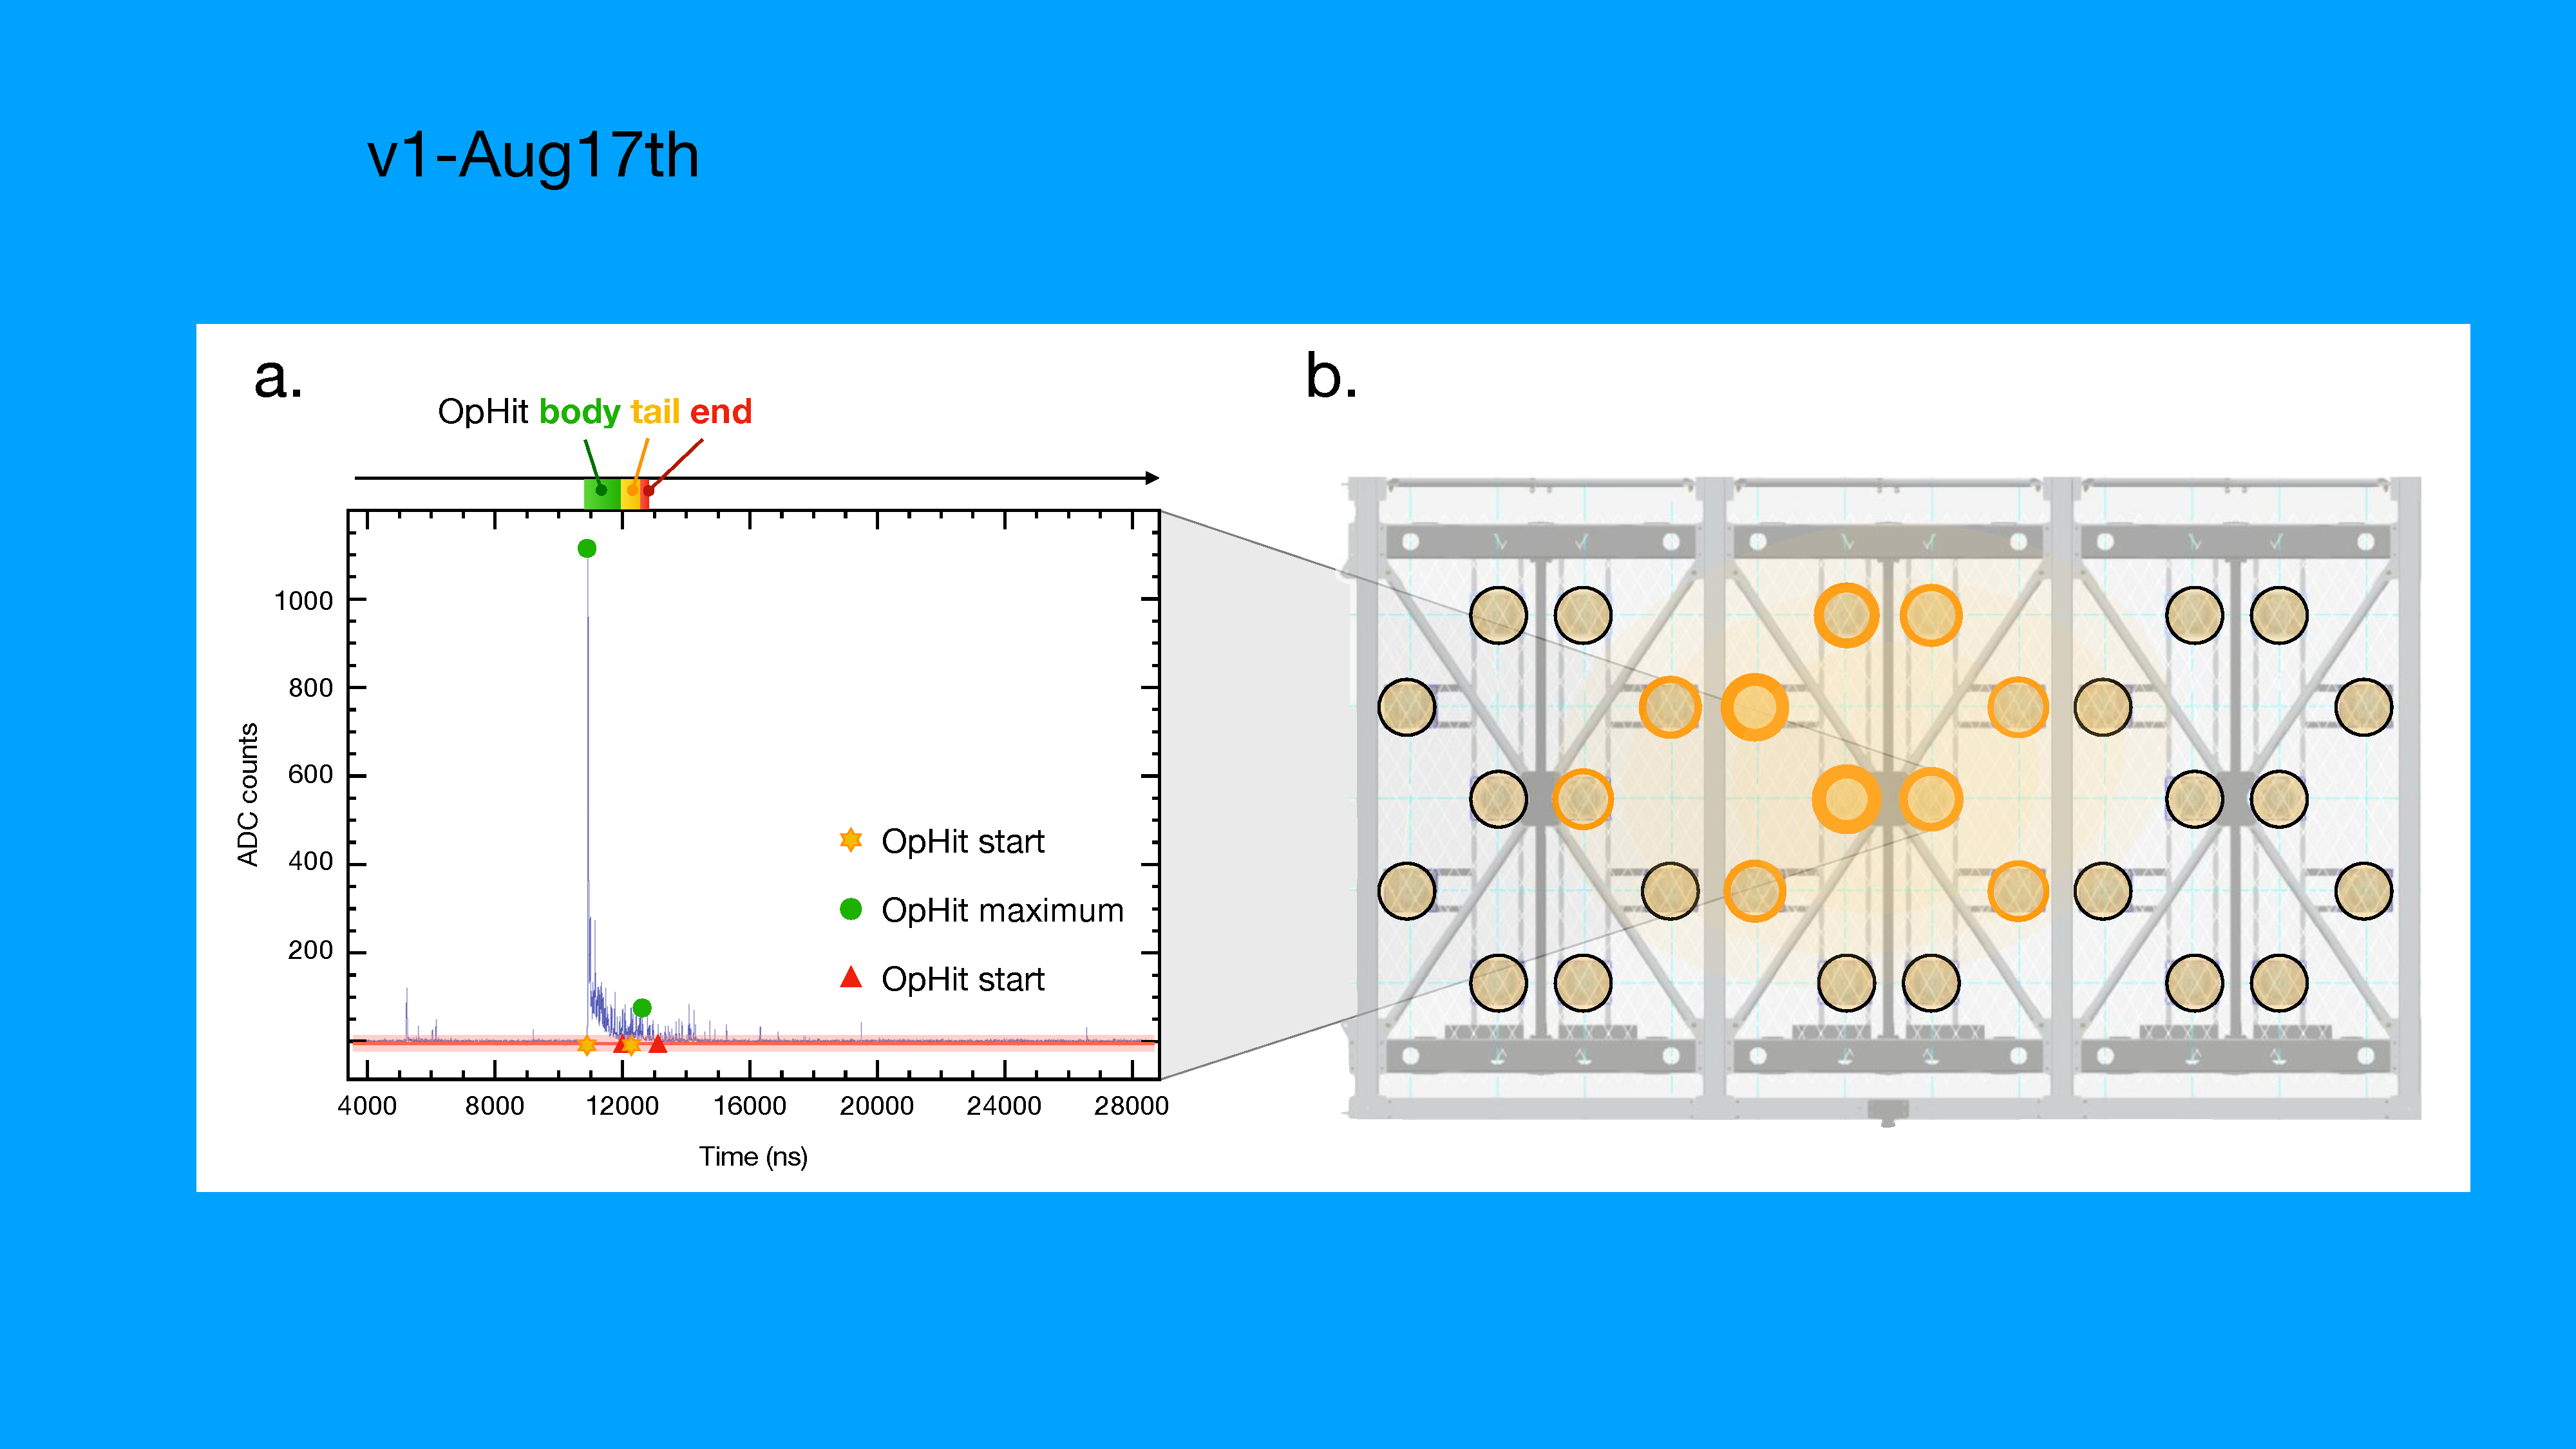
\includegraphics[width=\linewidth,trim={5.5cm 7cm 3.5cm 9cm},clip]{detector/PMT_reco.pdf}
    \caption[PMT reconstructed \emph{OpHits}]{Illustration of an interaction as seen by the PMTs inside the detector volume. (a) shows the pedestal-subtracted waveform produced by a single fired PMT, where the \emph{OpHit} information is marked on top, with the three regions (body, tail and end) highlighted. (b) shows all the PMTs activated during an event in the TPC volume; the PMTs collecting a light signal above the defined threshold are indicated in yellow. Their signal is used to build the so called \emph{OpFlash} object.}
    \label{fig:PMT_reco}
\end{figure}

\subsection{Cosmic ray tagger reconstruction} 

The first step in the reconstruction of the CRT signal is the extraction of the number of photoelectrons $n_\mathrm{p.e.}$. This is done starting from the raw ADC counts, subtracting the pedestal and correcting for the amplification gain \begin{equation}
    n_\mathrm{p.e.} = \frac{\mathrm{\#ADC} - \mathrm{ped}}{G}. 
\end{equation} 

A preliminary selection for the side CRT data is performed, requiring each signal to be above a \SI{7.5}{pe} threshold. Top CRT data are instead selected with a different requirement, i.e. a ``quadruple'' signal coincidence is necessary to generate a hit as shown in \autoref{fig:CRT_reco}(a). At this point it is possible to create the CRT \emph{Hit} objects for side and top CRTs. Two timestamps are associated to each hit: $T_0$ identifying the global timing of the recorded hit and provided by the White Rabbit switch system, and $T_1$ which identifies the relative timing of the hit with respect to the trigger. Additionally each CRT hit object has its position in the detector reference frame associated. Due to the differences in the CRT modules between side and top CRT, the position computation is slightly different. 

\begin{figure}
    \centering
    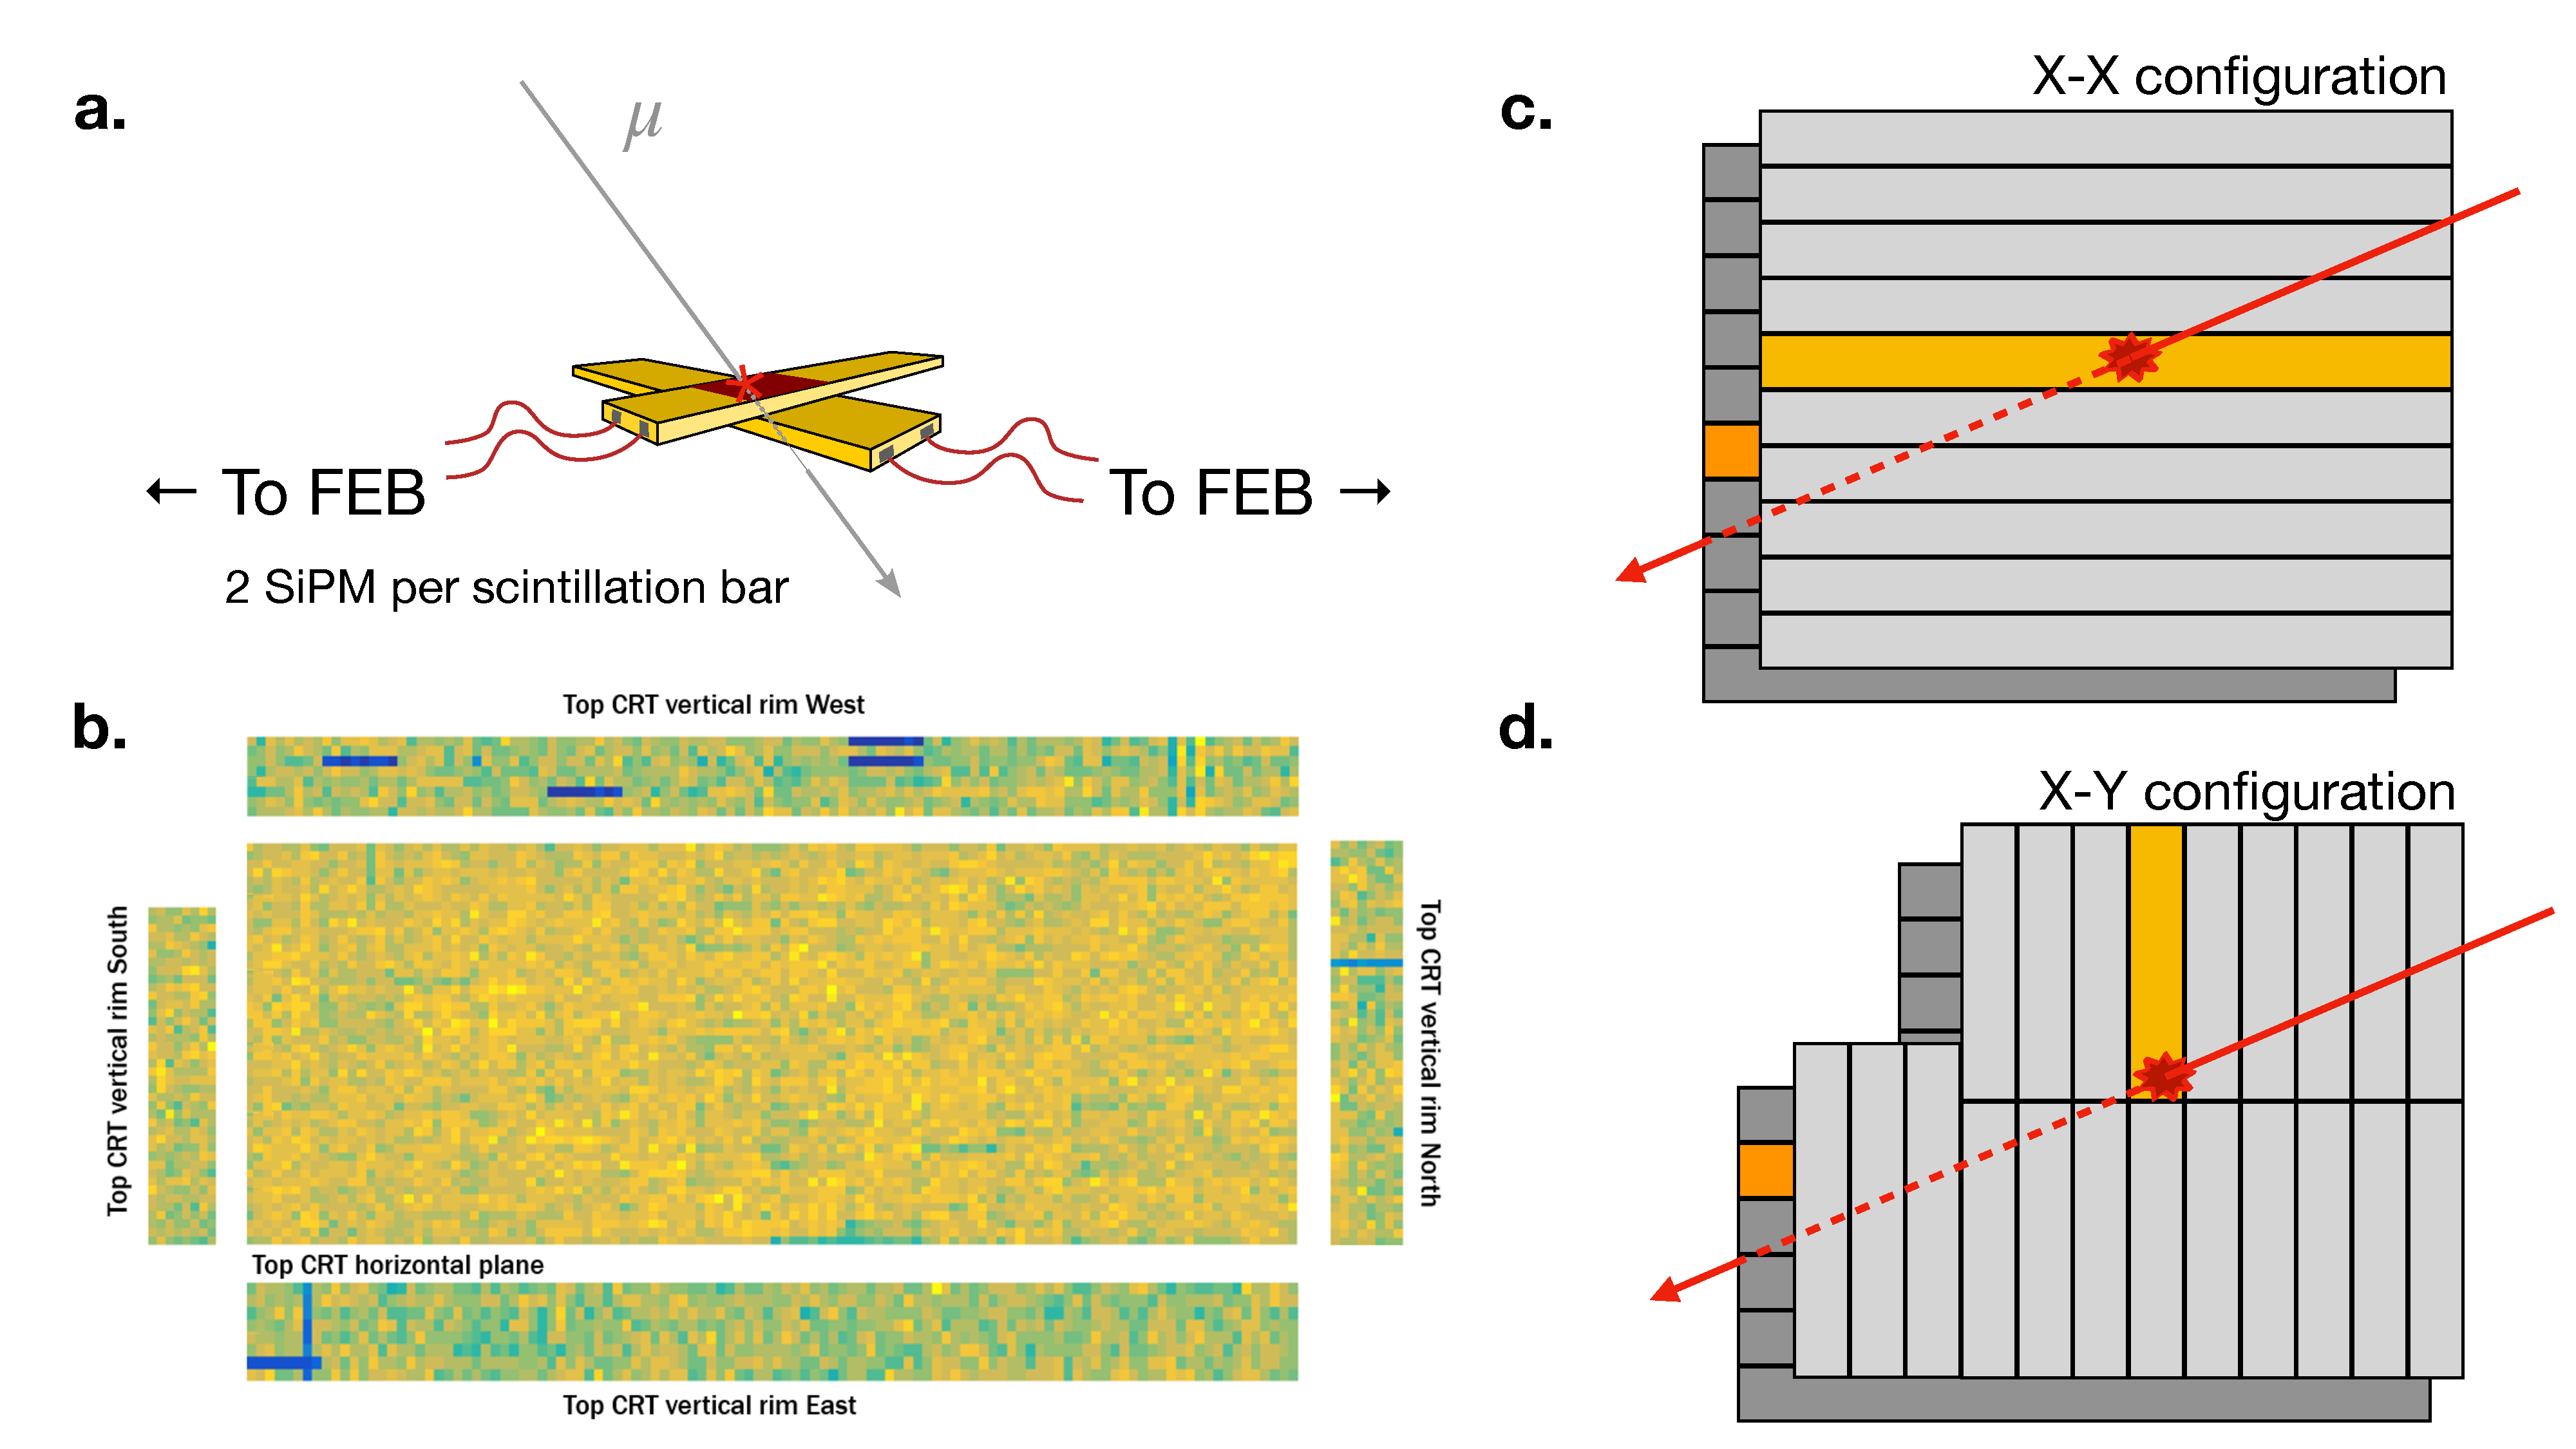
\includegraphics[width=\linewidth]{detector/CRT_all.pdf}
    \caption[CRT Hit reconstruction in space]{Illustration of CRT hit position reconstruction. (a) shows the reconstruction for the top CRT modules, where the coincidence between two scintillation bars is required. (b) shows the distribution of the CRT hits reconstructed in the different regions of the Top CRT. Blue regions correspond to malfunctioning channels. (c) and (d) show respectively the configuration fo the east/west and north side CRT, and south CRT modules. (b) is taken from \cite{Poppi:2023zmp}, (a), (c) and (d) are adapted from \cite{arteroponsStudyReconstructionNuMuCC}.}
    \label{fig:CRT_reco}
\end{figure}

By using the quadruple coincidence, the position of top CRT hits in each module is known with a granularity of \qtyproduct[product-units=power]{23x23}{\cm}. \autoref{fig:CRT_reco}(b) shows the distribution of the CRT hits using a collected calibration run. 

For the side CRT modules the position in the detector (reference) frame is reconstructed with a slightly different approach. The coincidence of adjacent layers is reconstructed offline via software because the same modules are being read by multiple FEBs. Hit scintillator strips are identified by selecting in each FEB the channel that generated the FEB trigger signal, which is the one with the highest charge amplitude. \autoref{fig:CRT_reco}(c) and d show two of the configurations of the CRT side module strips. The triggering strip is shown in yellow, and the red star shows the interaction point. The north, east and west side CRTs have the X-X configuration shown in \autoref{fig:CRT_reco}(c). For these components, if two opposite SiPM signals are collected within \SI{150}{\ns}, and read out by two FEBs, the longitudinal position (across the strip) can be computed with respect to the centre position of the strip by comparing the $T_0$ timestamps recorded by each FEB:     \begin{equation}
    z = \qty(T_B - T_A)/2 \cdot v_\mathrm{wls}, 
\end{equation} where $T_A$ and $T_B$ are, respectively, the two timestamps recorded by the FEBs  and $v_\mathrm{wls}$ is the group velocity of the light signal inside the wavelength shifter fibre. The south CRT wall instead was built with the X-Y configuration shown in \autoref{fig:CRT_reco}(d). In this case, a coincidence offline software-based approach similar to that used for the top CRT component is employed, by exploiting the orthogonal relative position of the outer and the inner strips. 

The last step performed in \emph{Stage0} concerns the temporal matching of the light and CRT information. This step is crucial, especially for higher-level processing, where it can be exploited to improve the efficiency by which correct interactions are selected inside the detector, rejecting out-of-time activity using the CRT-PMT match. 

\subsection{Wireplanes signal reconstruction}

The wire data is the waveform readout of the \num{53248} individual wires. The first step of the wire signal processing happens online directly on the readout cards installed in the TPC online computers, and aims at removing the coherent noise from the wires \cite{MicroBooNE:2017qiu}. Only minimal further processing is performed online, which leaves more scope for reprocessing the raw data using improved signal processing tools. The recorded waveforms are in ADC count/tick units, where the amplitude of the signal is expressed in ADC counts and the time information in ticks, each corresponding to \SI{0.4}{\us} in the ICARUS TPC timing. \autoref{fig:TPC_signal} shows a sample of the data collected by the three planes, exhibiting the characteristic bipolar shape for the two induction wire planes and a unipolar signal for the collection plane. 

\begin{figure}
    \centering
    \subfloat[]{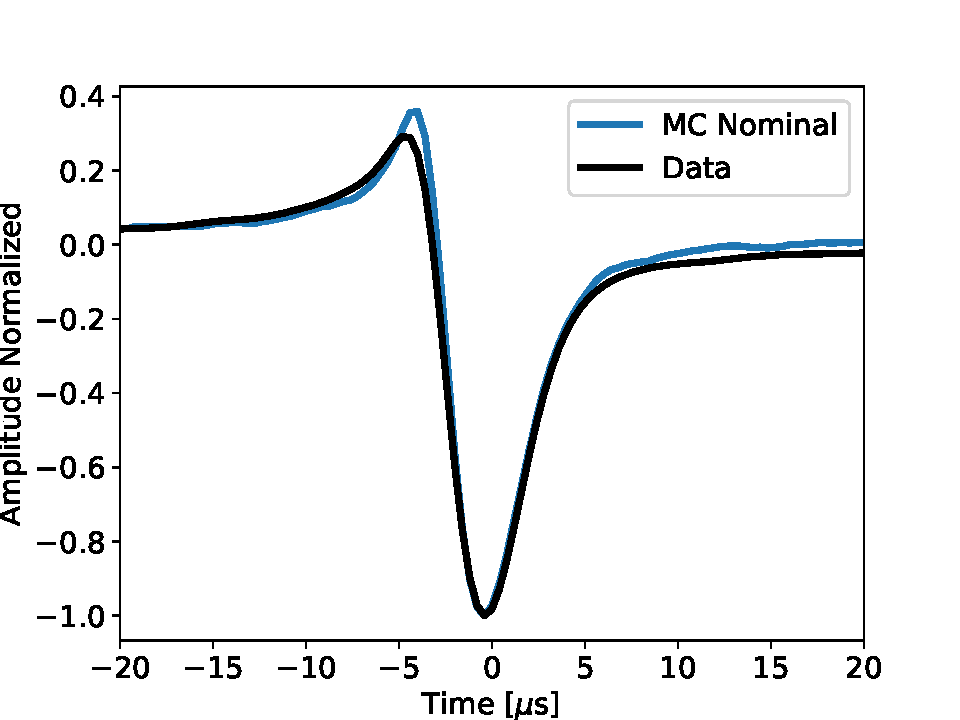
\includegraphics[width=0.3\linewidth]{detector/wvf_data_MCNominal_a20_P0.pdf}\label{fig:TPC_wire_i1}}
    \subfloat[]{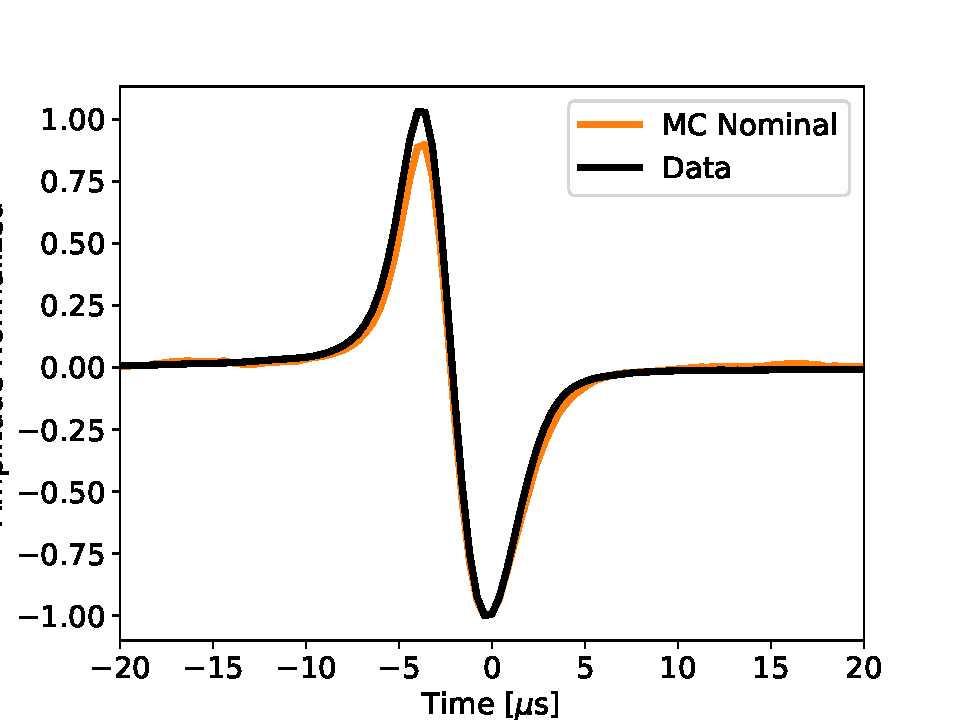
\includegraphics[width=0.3\linewidth]{detector/wvf_data_MCNominal_a20_P1.pdf}\label{fig:TPC_wire_i2}}
    \subfloat[]{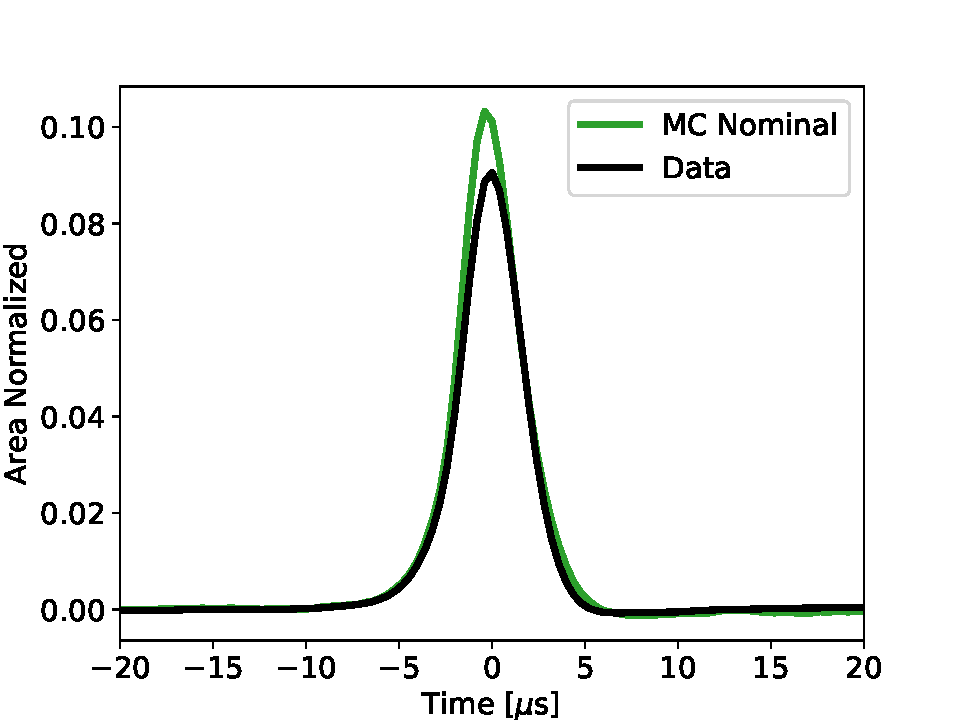
\includegraphics[width=0.3\linewidth]{detector/wvf_data_MCNominal_a20_P2.pdf}\label{fig:TPC_wire_c}}
    \caption[TPC plane signal]{Typical \emph{raw} signal captured by the three planes (induction-1 \ref{sub@fig:TPC_wire_i1}, induction-2 \ref{sub@fig:TPC_wire_i2} and collection \ref{sub@fig:TPC_wire_c}) showing the characteristic bipolar signal for the two induction plane and the unipolar shape for the collection plane. The signal is averaged in the $\theta_{xw}$ angle, where $x$ is the drift coordinate, and $w$ is the orientation of the wires in the $w$ plane. Picture taken from \cite{ICARUS:2024hmk}. }
    \label{fig:TPC_signal}
\end{figure}

In order to deconvolve the TPC wire signal from the deformation induced on the true signal by the electric field effects and shaping effects coming from the front end electronic, three major steps are addressed in \emph{Stage0}: \begin{inparaenum}
    \item the wire signals are deconvolved from the TPC electronic response functions, so that all three wire signal are also unipolar in shape;
    \item the signal is analysed in order to define the region-of-interest (ROI) with a threshold-based algorithm; 
    \item each ROI is finally fit using a Gaussian function, whose area is proportional to the number of drift electrons generating the signal. 
\end{inparaenum} Given the relevance of these steps of the processing chains, we will briefly describe them in the next paragraphs.

\paragraph{Wire signal deconvolution} The wire signal shape can provide information on the deposited charge of drift electrons and subsequently of the depositd enrgy of the particle interactiong in LAr. However, in order to explain such dependency, the effects related to the distorsion of the true signal, due to the drifting electric field and the electronic response, must be deconvolved from the readout signal. The readout signal $R(t)$ on the wires can be expressed as the convolution of serial effects of signal formation, electron propagation, electrostatic field response around the wires and processing by the DAQ to the true electronic signal, so that each wire channel response function can be factorised as \begin{equation}
    \begin{aligned}
        R(t, t')&=\mathrm{Ionization\ \otimes\ Recombination\ \otimes\ Diffusion\ and\ Attachment\ \otimes} \\
        &\quad \quad \quad \mathrm{Field\ response\ \otimes\ Electronic\ response\ \otimes\ Electronic\ noise}
    \end{aligned} 
\end{equation} In order to recover the desired ionisation electron yield, useful to measure the deposited energy per wire inside the detector as a function of time, it is necessary to unfold these effects. 

The ICARUS experiment exploits a signal processing chain similar to other LArTPC experiments, performing a deconvolution in time of the signal waveforms. Ideally, after the deconvolution step, the signal pulse produced by a charged track on the wire would be Gaussian-shaped, with an integral area proportional to the deposited charge, i.e. a proxy of the energy, inside LAr. The signal recorded on the wires is the convolution of the response function $R$ with the ``true'' $S$ signal, \begin{equation}
    M(t') = \int_{-\infty}^{+\infty} R(t,t')\ S(t)\ \dd t;
\end{equation} Using the properties of the Fourier transforms, this can be written in the frequency domain as $\mathcal M(\omega) = \mathcal R(\omega)\cdot \mathcal S(\omega)$, which can be inverted to extract the true wire signal $\mathcal S(\omega)$. This approach, referred to as ``one-dimensional'' deconvolution, is currently employed in most of LArTPC detectors. However, this assumes that the charge distribution on each wire is independent from the charge distribution on the wires in its vicinity. However, as shown in \cite{MicroBooNE:2018swd,MicroBooNE:2018vro}, it was demonstrated that this is not always true. Furthermore, while in general accounting for this effect implies small additional corrections to the overall deposited charge there are cases where wire channel correlations are non negligible. For example, for isochronous tracks (i.e. tracks lying parallel to the wires, which is frequent for the induction-1 wires given the specific ICARUS geometry), nearby wire channels correlation effects can create destructive interference patterns.

\begin{figure}
    \centering
    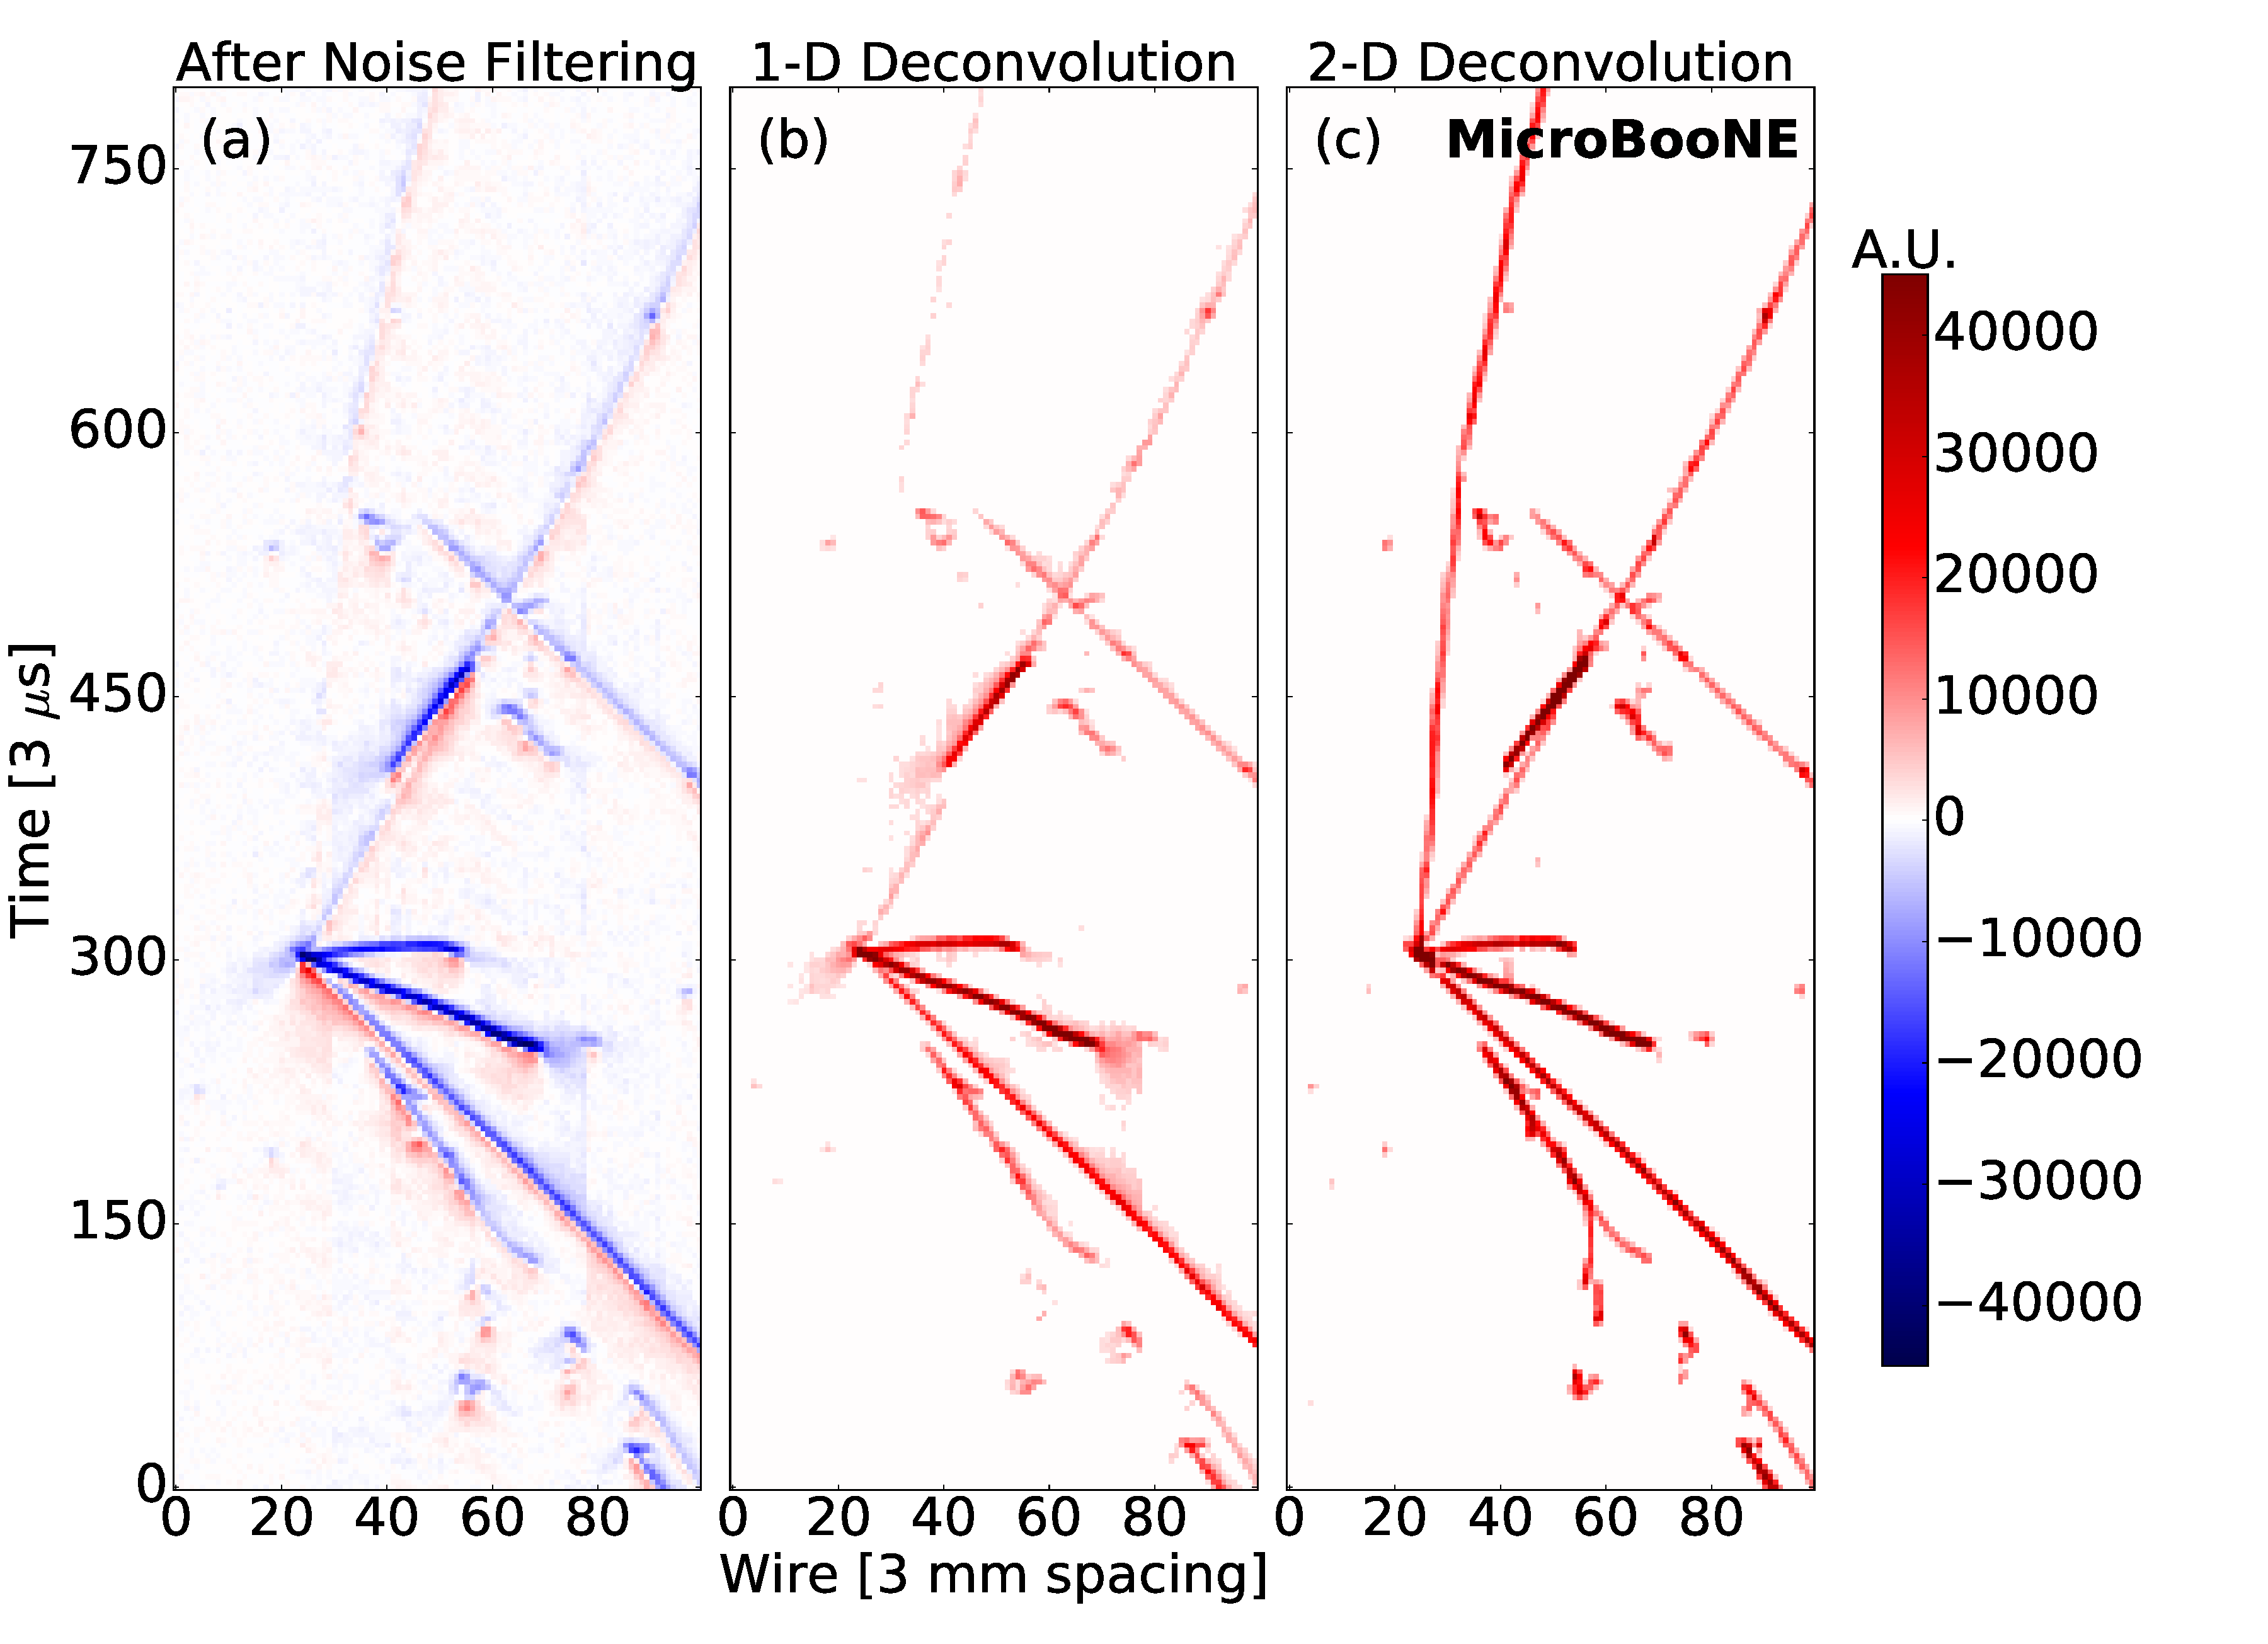
\includegraphics[width=0.85\linewidth]{detector/noiseVs1DVs2D.pdf}
    \caption[TPC signal processing]{Example of the effect of signal processing using the one-dimensional deconvolution approach employed in ICARUS (b) with respect to the noise-filtered data (a). Figure (c) shows the same event using a two-dimensional deconvolution approach, i.e. performing the deconvolution both in the time direction as well as in the direction of the wires. Picture taken from \cite{MicroBooNE:2018swd}. }
    \label{fig:uBooNE_signalProc}
\end{figure}

In \cite{MicroBooNE:2018swd,MicroBooNE:2018vro} a solution to this issue is presented: it consists in the application of two-dimensional deconvolution techniques where both time and wire channel are taken into account. This provides a strong and computationally efficient method to better extract the distribution of ionisation electrons. \autoref{fig:uBooNE_signalProc} shows the result of the 1D and 2D approaches as tested by the MicroBooNE experiment. Efforts aimed at adapting two-dimensional deconvolution techniques to ICARUS TPC raw data and testing their impact on the reconstruction performance are currently ongoing. Preliminary results indicate a remarkable enhancement in reconstruction efficiency specifically for track-like particle trajectories.

\paragraph{ROI finding} After the deconvolution, we need to identify interesting regions of the TPC wire signals as function of time. With a threshold-based algorithm we find the interesting regions (ROIs) to look for the signal hits, i.e. segments of waveform corresponding to the signal. ROIs can be actually relevant to iteratively improve the performances of the 1D/2D deconvolution steps, by minimising the time-domain region over which the deconvolution is performed. Once ROIs are identified, a baseline ADC counts value can be assigned to all the remaining times in the waveform, thereby drastically reducing the size of these data products inside the data files. 

\paragraph{Gaussian \emph{Hit} creation} Upon the identification of ROIs, the final step is the creation of the \emph{Hit}s objects. A \emph{Hit} is a two-dimensional object representing a cluster of electric drift charges, arriving at a certain time on a certain wire. The hit-finding algorithm runs under the assumption the distribution of the drift charges is Gaussian. Operating on the deconvolved ROI segments of the waveforms, it tries to fit one or multiple Gaussian distributions onto the signal shape. The parameters derived from the Gaussian fit are properties of the hits and include the area under the Gaussian(s), mean and FWHM of the distribution and its multiplicity. The area corresponds to the cumulative charge deposited by the electrons and proportional to the deposited energy inside the detector; the mean and the FWHM represent the hit peak time and its width. 

At this point, a collection of 2D hits for each plane of wires is available. For each reconstructed event, the three 2D views of the planes are stored and used as input for the event reconstruction taking place inside \emph{Stage1}. 

\section{TPC event reconstruction} \label{sec:TPC_reco_gen}

\emph{Stage1} is dedicated to performing the high-level event reconstruction, taking the \emph{Hit} objects created by the modules of \emph{Stage0} and transforming them to build the full interaction picture. This part of the event reconstruction interests primarily the information extracted from TPC and PMT sub-detectors, since it is expected for most neutrino interactions (${\sim}\SI{80}{\percent}$) to be contained inside the LAr volume, hence not expected to generate a CRT signal. 

To perform the event reconstruction inside the TPC, the starting point is given by the three collections of 2D hits created in \emph{Stage0}.

The hit-finding algorithm, providing the collections of 2D hits, is optimised to prefer efficiency over purity, reaching an efficiency greater than \SI{99}{\percent}; this might, however, lead to the creation of non-physical hits, especially in very noisy regions, that might cause failures in the pattern recognition steps. To prevent such problems, the collection of 2D hits produced by the hitfinding algorithm are filtered using the \emph{Cluster3D} algorithm. This preliminary step of the \emph{Stage1} reconstruction runs over the set of wires of the three planes and, exploiting the common $x$ drift coordinate, looks for time-correlated hits across the three planes. If matches are not found, or hits are isolated, then they are filtered out. The resulting filtered collection of hits is used as the input for the subsequent high-level reconstruction tools that are, in the contex of the ICARUS experiment, the Pandora topological reconstruction \cite{MicroBooNE:2017xvs} and the SPINE machine-learning-based recontruction \cite{Drielsma:2021jdv}. 

% This thesis focuses on developing tools for the event reconstruction process briefly described below, which is referred to as ``Pandora event reconstruction'' within the collaboration. However, recent inroads in Computer Vision (CV) and Machine Learning (ML) have motivated a new approach to the analysis of particle imaging detector data. Additionally, having multiple different approaches to event reconstruction can be crucial in proving the robustness of each one. 

% This thesis is mostly geared toward the Pandora event reconstruction, of which an in-depth description is provided in \autoref{sec:Pandora} and subsequent sections. In \autoref{sec:SPINE} is also provided a description of the SPINE reconstruction framework. 

Pandora has been the baseline for the event reconstruction within the SBN program since its first days. The Pandora reconstruction chain takes the three 2D hits produced by the hit-finding algorithm as input, filtered by the cluster3D tool, performing a topological reconstruction of the tracks and showers taking part in the interaction to allow a hiearchical reconstruction of the neutrino candidate events. It specifically promotes the idea of a multi-algorithm approach to solving pattern-recognition problems. In this approach, the input building blocks (hits) describing the pattern recognition problem are considered by large numbers of decoupled algorithms. Each algorithm targets a specific event topology and controls operations such as collecting hits together in clusters, merging or splitting clusters, or collecting clusters in order to build a representation of reconstructed particles in the detector. The algorithms gradually build up a picture of the underlying events and collectively provide a robust reconstruction. % Further details are provided in \autoref{sec:Pandora}. 


Recent inroads in Computer Vision (CV) and Machine Learning (ML) have motivated a new approach to the analysis of particle imaging detector data, and efforts within the ICARUS collaboration have been made to develop a machinel-learning-based approach to the event recosntruction. SPINE (Scalable Particle Identification with Neural Embeddings) project serve this purpose. Unlike the Pandora reconstruction, which starts from the 2D colection of hits on the readout planes, the SPINE reconstruction leverage a fully three-dimensional reconstruction starting from the 3D space points created by the cluster3D algorithm. This way ambiguities that might arise in the Pandora reconstruction are resolved. However, this approach introduces other difficulties, as will be addressed in dedicated paragraphs. 

This thesis has the aim of performing a detailed validation study of the Pandora-based event reconstruction, and so a more detailed descritpion is given in the sections following \autoref{sec:Pandora}. The SPINE approach to the event reconstruction is briefly presented and discussed in \autoref{sec:SPINE}.

\subsection{Geometry of the ICARUS detector}

The Pandora reconstruction --- as any reconstruction paradigm for LArTPC would do --- heavily exploits the geometrical characteristic of the detector. Newer LArTPC detectors employ a common geometry to make it effortless to transition the software codebase from one to another. Being the first of its kind and since its original physical scope extended beyond that of the SBN program, the ICARUS detector TPC geometry is unique. As already mentioned in \autoref{sec:ICARUS_T600}, and illustrated in \autoref{fig:i2_c_planes_wirepitch_detail}, ICARUS wire planes have some peculiarities. First, the wire orientation is different from other LArTPCs currently in use for neutrino experiments, including SBND and ProtoDUNE: for reasons related both to mechanical constraints and topological reconstruction, it is customary to build TPC wire planes with wires oriented \SI{+-60}{\degree} with respect to the vertical direction for the first two induction planes ($u$/$v$), and have the collection ($w$) plane wires vertical, whereas in the ICARUS detector the first induction plane features horizontal wires, and the second induction and collection planes are oriented \SI{+-60}{\degree} with respect to the horizontal. The reason for the horizontal wires was dictated by the target physics analyses for the ICARUS experiment at LNGS, especially for the detection of cosmic-induced particles. Due to mechanical limitations, however, it was not possible to have \SI{18}{\metre} long wires kept at the tension needed for the detector operation, so they had to be split into two 9-meter-long sections. 

The geometrical parameter that is core for the Pandora software when performing the 3D reconstruction of the wire planes 2D projections is the angle at which the wire planes are oriented. This information is used to perform the spatial reconstruction of the hits collected in the different planes, using projective geometry. In Pandora each plane is associated to a so called view and each view has associated the angle at which wires are oriented. In most LArTPCs the mapping between views and planes is univocal. For example, considering the SBND APA, both East and West APAs feature the $u$ plane at $+\SI{60}{\degree}$, the $v$ plane at $-\SI{60}{\degree}$ and the $w$ plane at \SI{0}{\degree} with respect to the vertical direction. In the ICARUS TPC, however, the requirement to have the induction-2 and collection plane's wire angle oriented in the same direction if seen in the drifting direction (see, for reference, \autoref{fig:i2_c_planes_wirepitch_detail}) means that the mapping is not unique and depends on which TPC of each T300 module is being considered. As the association between the readout plane and view is not guaranteed in the ICARUS geometry, except for the induction-1 plane, there are some caveats with the Pandora reconstruction. This is the case, for example, when the reconstruction assumes that the $w$ view is the collection plane. For some steps of the current reconstruction, this step has been addressed. 

\subsection{Pandora approach to the event reconstruction} \label{sec:Pandora}

As already anticipated, Pandora takes an innovative approach to the topological event reconstruction, splitting the problem of pattern recognition among the action of smaller, decoupled algorithms. The Pandora framework is embedded inside \emph{LArSoft} and accessed via the \emph{LArPandora} module, that handles the Pandora event reconstruction. The ICARUS detector consists of two separated T300 modules; thus, two parallel instances of the Pandora reconstruction are run on each event, corresponding to the east and west cryostats. Each Pandora instance runs the full list of algorithms on the corresponding T300 module. 

The inputs are the collections of 2D hits in the $x$--wire plane, with $x$ representing the drift time and the second coordinate being the wire number. The $x$ coordinate is common across the views and thus is exploited to match the hits from different planes. The output of the pattern recognition algorithms are the Particle Flow Particles, or PFParticles, objects; each PFParticle correspond to a distinct track or shower, and, through the action of subsequent algorithms, is associated to a list of 2D clusters, which are groups of hits on the same plane belonging to the same reconstructed object. Each PFParticle is also associated with a set of 3D positions (named SpacePoints) corresponding to the reconstructed 3D trajectory and with a vertex position, defining its interaction point or its first energy deposition. PFParticles are finally arranged in a hierarchy, which identifies parent-daughter relationships for a given interaction candidate. For each interaction defined as neutrino-like, one empty PFParticle is created, identifying the neutrino PFParticle, and thus associated with the primary interaction vertex. \autoref{fig:LArPandora_dependencies} shows all data products produced by Pandora and their interdependency. 

\begin{figure}
    \centering
    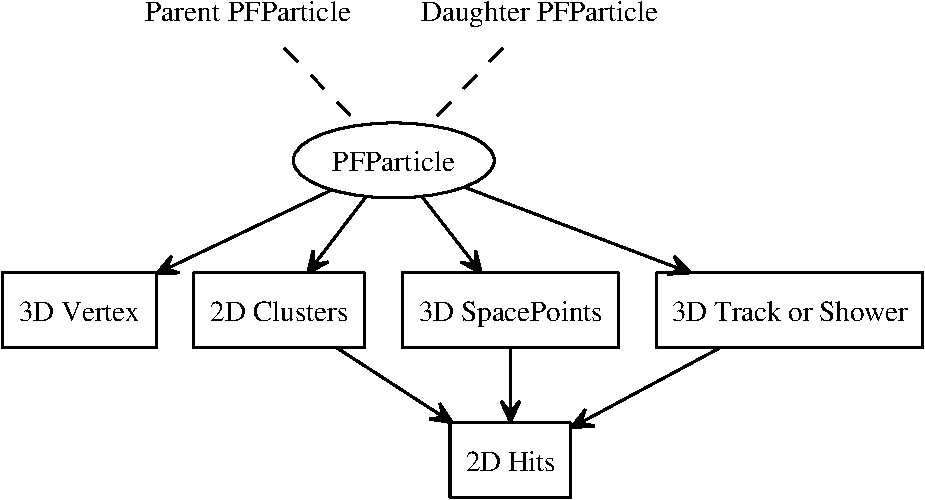
\includegraphics[width=0.75\linewidth]{pandora/LArSoftOutput.pdf}
    \caption[LArPandora output data products]{The Pandora output data products. Navigation along PFParticle hierarchies is achieved using the PFParticle interface, represented by dashed lines. Navigation from PFParticles to their associated objects is represented by solid arrows. Picture taken from \cite{MicroBooNE:2017xvs}. }
    \label{fig:LArPandora_dependencies}
\end{figure}

Three Pandora multi-algorithm reconstruction paths have been created for use in the analysis of ICARUS data: PandoraFastReco, PandoraCosmic and PandoraNeutrino. The last two are, as the names suggest, aimed at the reconstruction of precise interaction topologies; namely,  PandoraCosmic is optimised for the reconstruction of cosmic-ray muons and their daughter delta-rays, whereas PandoraNeutrino is optimised for the reconstruction of neutrino interactions. The PandoraFastReco path is run prior to both PandoraNeutrino and PandoraCosmic, with the precise aim of identifying and excluding from further processing steps \emph{unambiguous} cosmic-ray muons, employing a faster reconstruction pipeline. The output of the PandraFastReco path corresponds to a list of candidate cosmic rays. This list is then examined by a tagging module which identifies unambiguous cosmic-ray muons, based on their topological features, and removes their hits from the list. This enables an initial coarse separation of candidate signal events from background, thereby restricting the use of complex topological reconstruction algorithms to the most interesting events and reducing the overall computational cost of the reconstruction chain. \autoref{fig:pandora} illustrates the subsequent steps applied to each event by the Pandora reconstruction. 

% \begin{sidewaysfigure}
%     \centering
%     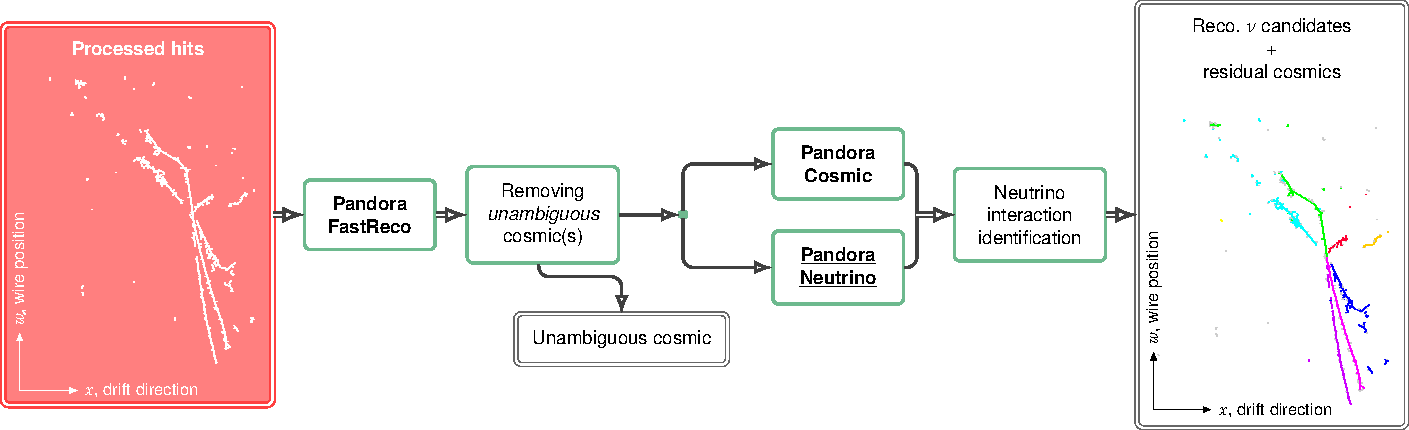
\includegraphics[width=\linewidth]{pandora/figure_Pandora/pandora.pdf}
%     \caption[Overview of the Pandora reconstruction chain]{Illustration of the Pandora reconstruction chain. Starting from a set of image-like collections of 2D hits, as shown in the left red panel, the approach is to first address a fast and rough reconstruction, aimed at removing the particles that are clearly cosmic-ray muons. Then each interaction inside the detector is passed through both PandoraCosmic and PandoraNeutrino chains to refine its reconstruction. }
%     \label{fig:pandora}
% \end{sidewaysfigure}

\begin{figure}[p]
    \centering
    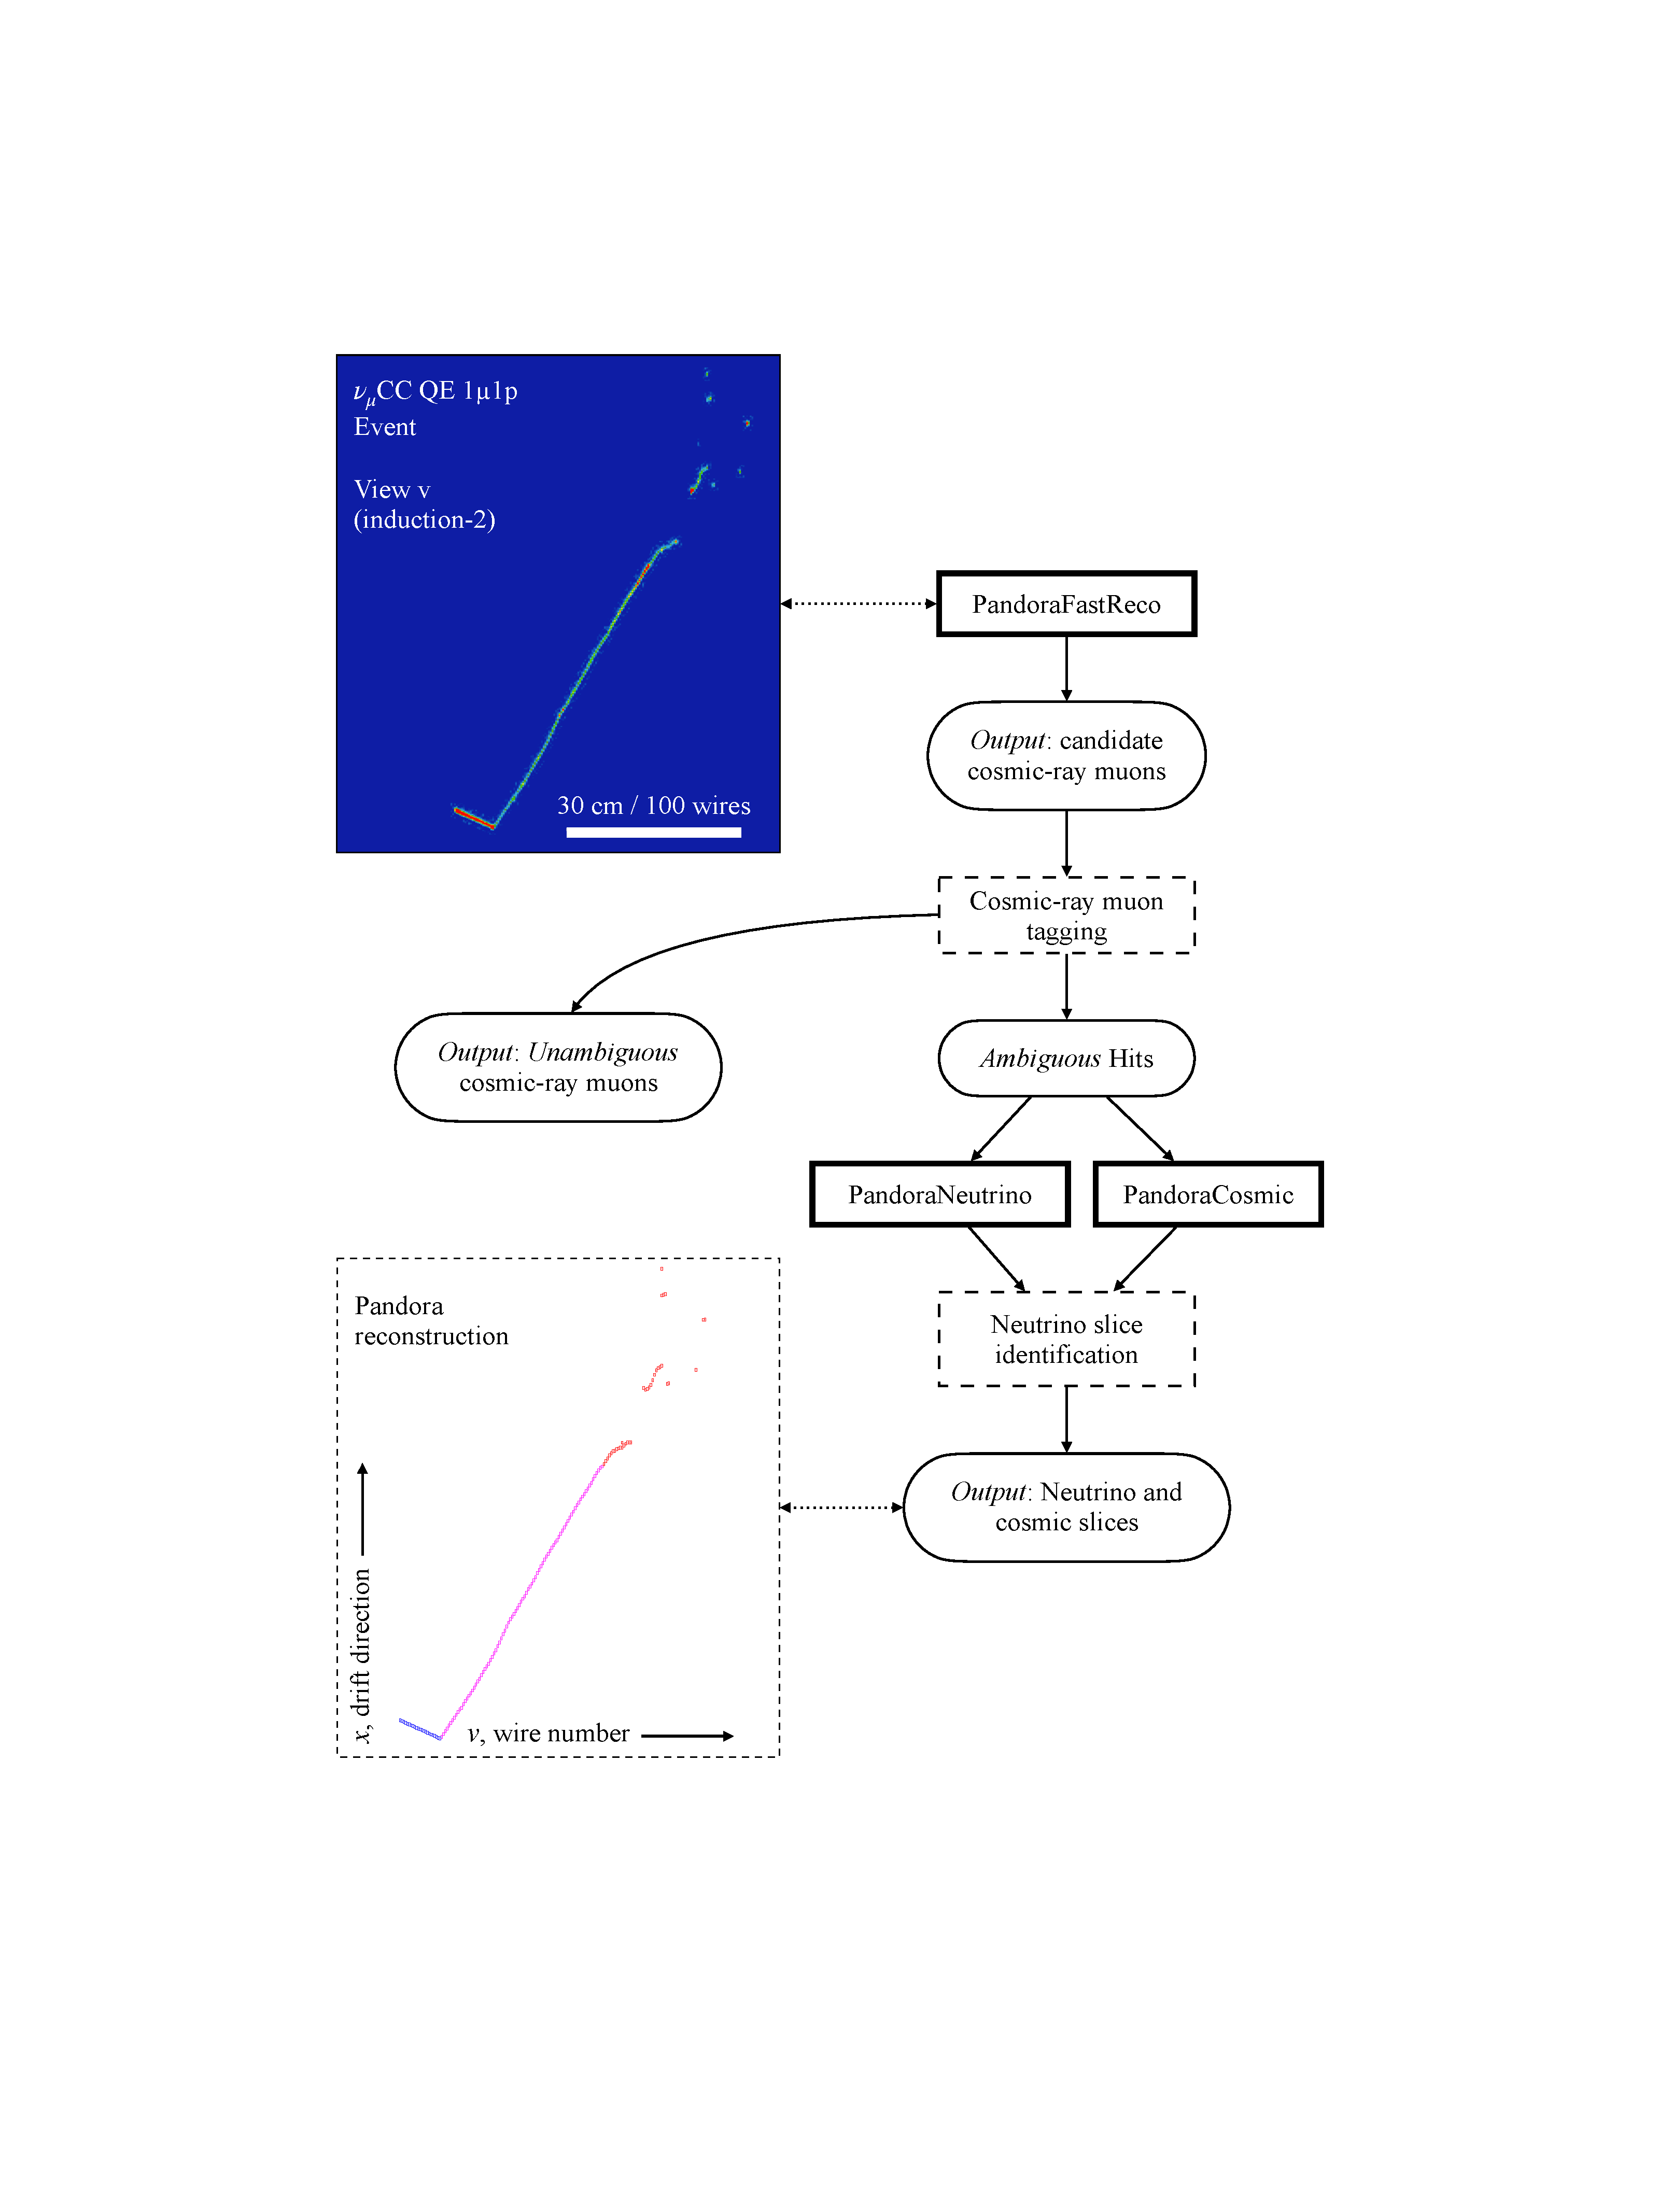
\includegraphics[width=0.95\linewidth, trim={9cm 14cm 9cm 12cm}, clip]{pandora/figure_Pandora/PandoraFull.pdf}
    \caption[Overview of the Pandora reconstruction chain]{Illustration of the Pandora reconstruction chain. Starting from a set of image-like collections of 2D hits, as shown in the event display in the top panel, the approach is to first address a fast and rough reconstruction (PandoraFastReco), aimed at removing the particles that are clearly cosmic-ray muons. Then each interaction inside the detector is passed through both PandoraCosmic and PandoraNeutrino chains to refine its reconstruction. }
    \label{fig:pandora}
\end{figure}

\subsection{PandoraFastReco: \emph{unambiguous} cosmic hits removal} \label{sec:fast_reco}

The first Pandora reconstruction path applied to the events consists of a set of tools aimed at performing a coarse reconstruction of all the hits identified during the readout window. This way, long straight tracks coming from muons crossing the detector volume are identified. A list of ``unambiguous'' cosmic-ray particle is created, using a classification of these reconstructed objects on the basis of topological considerations. The PandoraFastReco step shares most of the algorithms with the PandoraCosmic reconstruction path, since the goal is similar and entails the reconstruction of interactions characterised by a long straight track, usually crossing the full detector volume. The path, illustrated in \autoref{fig:PandoraFastReco}, is composed of four main stages, that are the subject of the next paragraphs. 

\begin{figure}
    \centering
    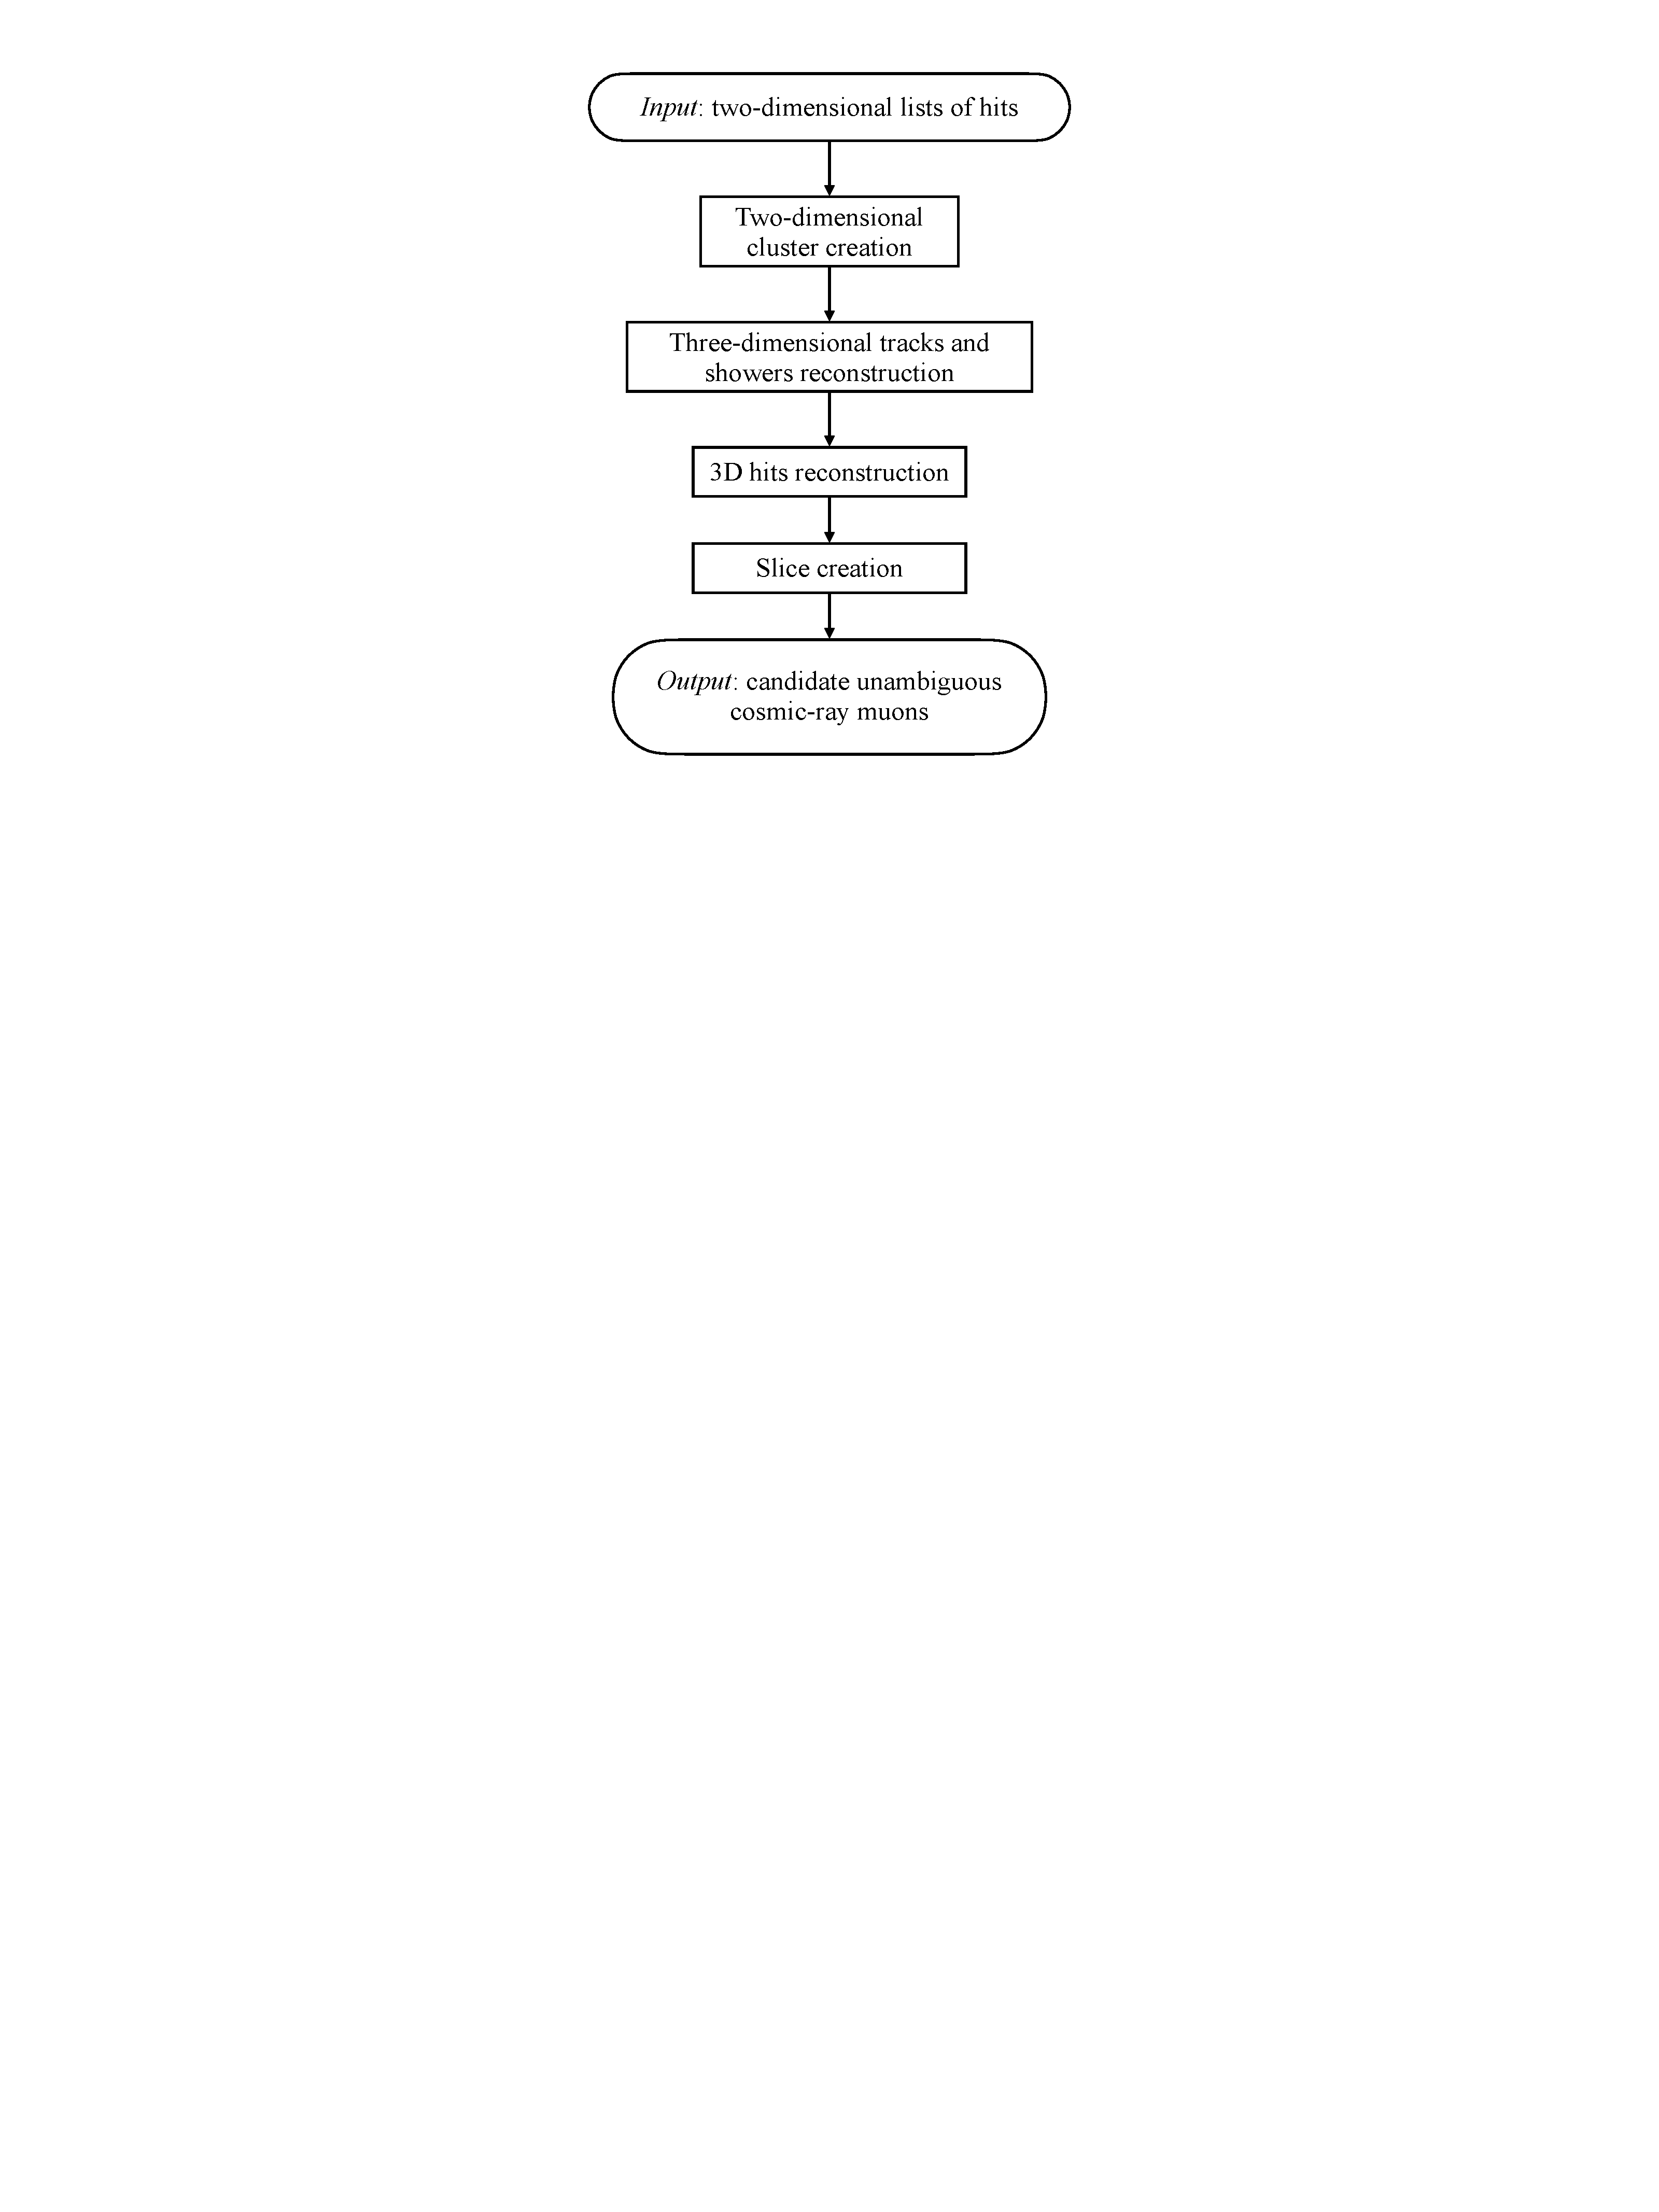
\includegraphics[width=0.5\linewidth,trim={16cm 47cm 16cm 1.5cm}, clip,page=1]{pandora/Pandora.pdf}
    \caption[PandoraFastReco path illustration]{Illustration of the main steps of the PandoraFastReco path, which is applied as a first coarse reconstruction. This path aims at creating unambiguous cosmic-ray muon candidates that are then flagged and whose hits are excluded from further processing. Figure adapted from \cite{MicroBooNE:2017xvs}}
    \label{fig:PandoraFastReco}
\end{figure}

\subsubsection{Two-dimensional reconstruction}

The first step takes as input the three separate lists of two-dimensional hits, corresponding to the three views or wire planes. For each, the TrackClusterCreation algorithm creates bidimensional clusters of hits, representing continuous lines of hits. Bifurcations, kinks or any topological branch-like feature stop the creation of a cluster and start the creation of another cluster. This approach ensures that clusters of hits created at this level have high purity, meaning a high number of correctly associated hits at the expense of completeness, meaning that a single true particle could be split into multiple clusters. At this point, cluster-merging algorithms identify associations between different 2D algorithms, improving the track completeness and affecting its purity in a minor way. Additionally, algorithms aimed at stitching together clusters that are split due to unresponsive wires or hits under the reconstruction threshold (that are not reconstructed) come into play at this level. 

To improve purity, cluster splitting algorithms refine the selection by breaking simple clusters if topological features indicate that there are ``spurious'' hits inside the cluster. 

\subsubsection{Three-dimensional reconstruction}

After 2D clusters are created, they are collected together with the aim of creating groups of 2D clusters that represent the same individual track particle. The challenge these algorithms need to address is to identify consistent groupings of clusters from the different views. The 3D track reconstruction is performed by three main algorithms: the ThreeDTransverseTracks algorithm, the ThreeDLongitudinalTracks algorithm and the ThreeDTrackFragments. The former algorithm has the biggest impact on three-dimensional track reconstruction.

The ThreeDTransverseTracks algorithm identifies all the suitable combinations of clusters from the three readout planes and inspects these combinations to identify cluster-matching ambiguities. These ambiguities are then used to improve the 2D cluster iteratively and remove them. The groupings of three clusters from the three readout planes are created by exploiting the common $x$ drift coordinate. On each view sliding fits are performed on the clusters; given a point on the $x$ coordinate, then the position of the sliding fit on two of the three views can be extracted, for example, the position on the $u$ and $v$ views. These positions, together with the coordinate transformation plugin, can be used to predict the position of the third cluster --- in the example shown in \autoref{fig:PandoraThreeDTracks}, in the $w$ view --- at the same $x$ drift coordinate. This prediction can be compared to the sliding fit position on the third view, and the same can be done with all possible combinations --- $u,v\to w$; $v,w\to u$ and $w, u \to v$. By performing such fits, and therefore checking the possible groupings of clusters across the three views, connections between them are created. The goal is to make these connections unambiguous, i.e. no two unique clusters from the same view are associated to the same unique cluster on another view. As described in \cite{MicroBooNE:2017xvs}, multiple tools query the different connection types across the views. Once no ambiguities are observed in the sets of clusters, the algorithm passes a list of sets of two (or three) clusters from different views to the following algorithms. Two examples showing how these tools operate on the 2D clusters are shown in \autoref{fig:PandoraThreeDTracks}. 

\begin{figure}
    \centering
    \subfloat[]{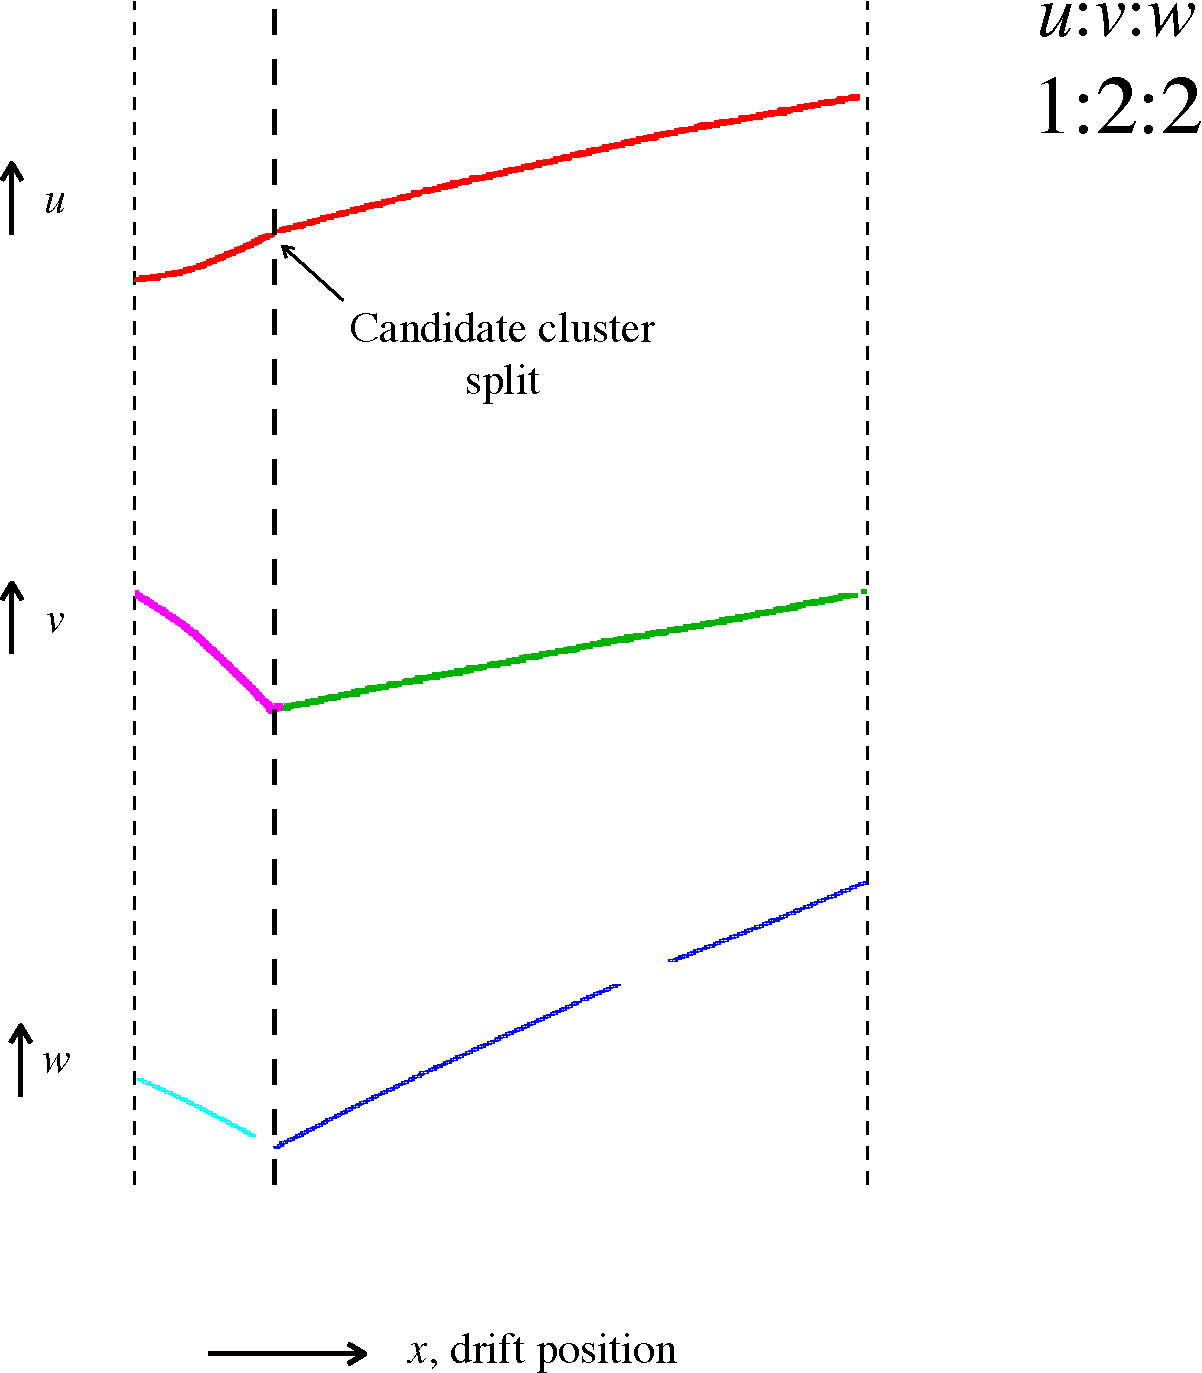
\includegraphics[width=0.5\linewidth]{pandora/ThreeDTracksTools/OvershootTracksTool.pdf}\label{fig:OvershootTracksTool}}
    \subfloat[]{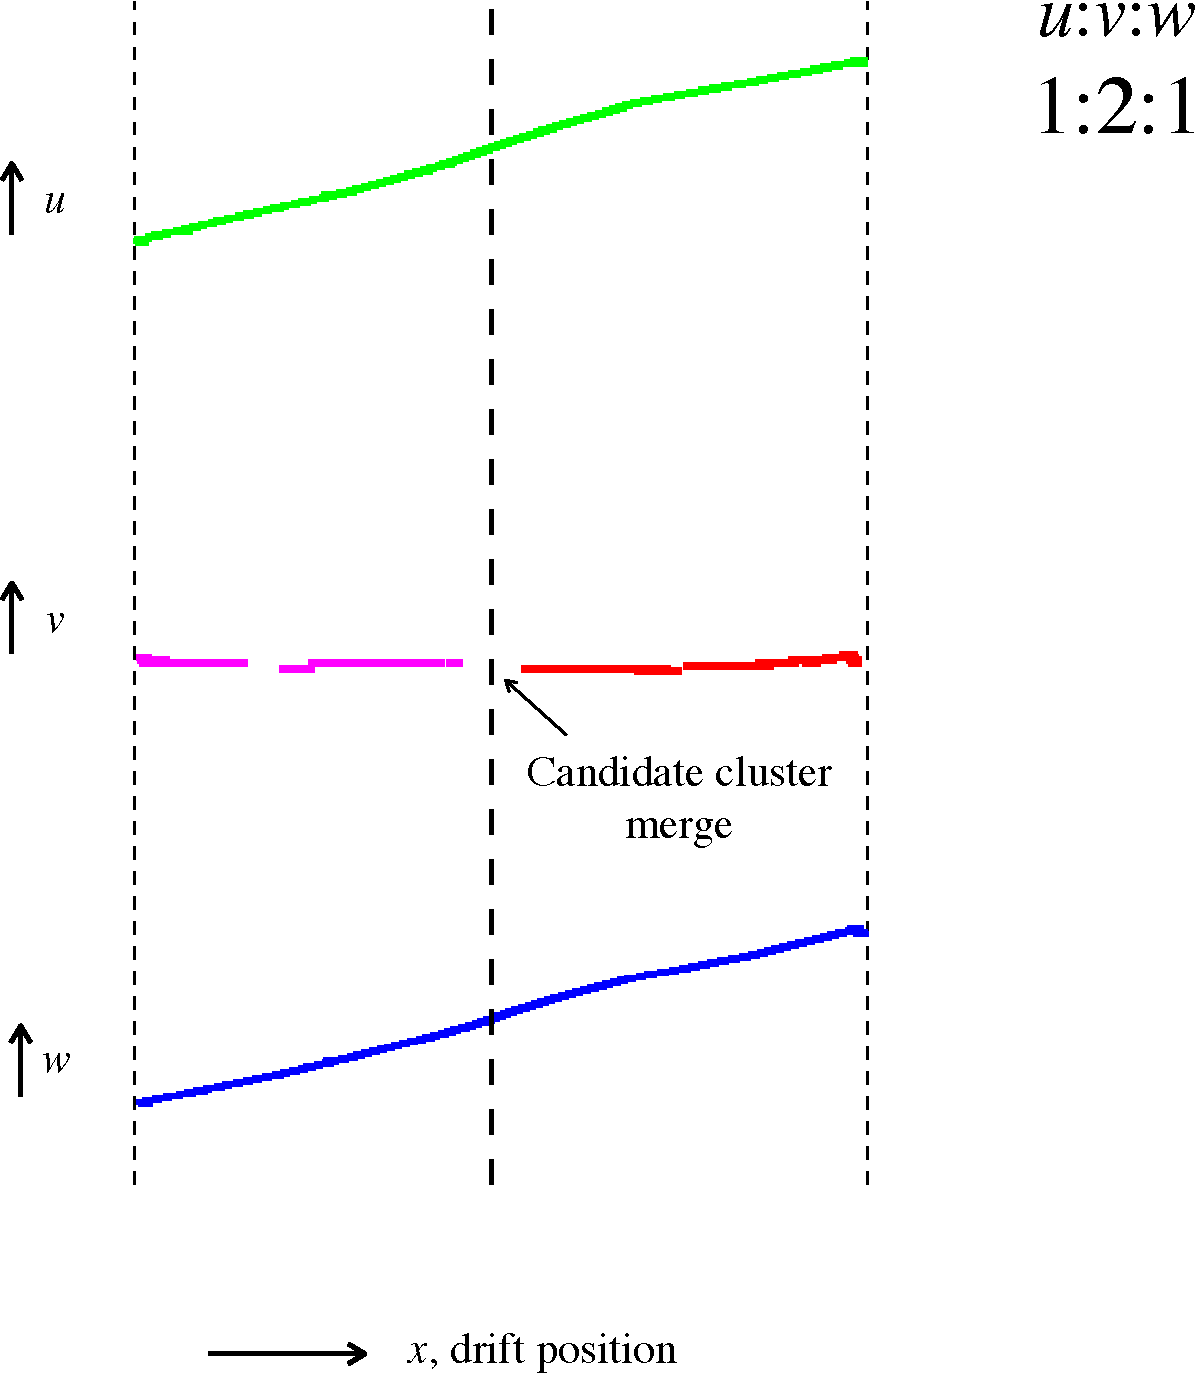
\includegraphics[width=0.5\linewidth]{pandora/ThreeDTracksTools/UndershootTracksTool.pdf}\label{fig:UndershootTracksTool}}
    \caption[Three-dimensional reconstruction helper tools]{Example of two of the tools querying the 2D clusters' connections. \ref{sub@fig:OvershootTracksTool} aims at resolving the ambiguities that arise from one view having two clusters merged into one. This ambiguity is resolved by splitting the cluster with the information from the other two views. \ref{sub@fig:UndershootTracksTool} has the opposite role and has the goal of merging cluster erroneously split into multiple pieces at previous stages. }
    \label{fig:PandoraThreeDTracks}
\end{figure}

\subsubsection{Three-dimensional hit reconstruction}

At this point, the assignment of hits to reconstructed particles is complete, each particle containing hits from two or usually three views. For each 2D hit a 3D point is created, with multiple approaches depending on the cluster topology. In all cases, the common step is the minimisation of a $\chi^2$-like value to get the best $y,z$ values for a given $x$ coordinate. 

After the 3D hit creation, candidate muon cosmic-ray particles are created, and they are tagged to filter out hits belonging to the unambiguously cosmic-ray particles. The remaining filtered hits are passed to subsequent paths of the reconstruction, namely PandoraCosmic and PandoraNeutrino. 

\subsection{PandoraNeutrino: topological neutrino event reconstruction} \label{sec:PandoraNeutrino}

A key requirement for the PandoraNeutrino reconstruction path is that it should be able to deal with the presence of cosmic-ray muon remnants. The approach to address this problem is therefore to run the same 2D clustering, 3D cluster matching and 3D hit reconstruction described in \autoref{sec:fast_reco}. After this path is run, 3D hits are divided into \emph{slices}, which are separate lists of clusters of lists, using proximity-based metrics. For a given event, the idea is to isolate the candidate neutrino interaction from any leftover cosmic-ray induced-tracks. The original 2D hits associated with each slice are then used as an input to the dedicated neutrino reconstruction, which is described in this section. 

The PandoraNeutrino dedicated reconstruction (shown in its entirety in \autoref{fig:PandoraCosmicNeutrino}\ref{sub@fig:PandoraNeutrino}) begins with a track-oriented clustering algorithm and a series of topological algorithms. Before processing the 2D clusters, the interaction vertex is reconstructed. 

\begin{figure}
    \centering
    \subfloat[]{\includegraphics[width=0.5\linewidth,trim={16cm 41cm 16cm 1.5cm}, clip,page=2]{pandora/Pandora.pdf}\label{fig:PandoraCosmic}}
    \subfloat[]{\includegraphics[width=0.5\linewidth,trim={16cm 40cm 16cm 1.5cm}, clip,page=3]{pandora/Pandora.pdf}\label{fig:PandoraNeutrino}}
    \caption[PandoraCosmic and PandoraNeutrino paths illustration]{\ref{sub@fig:PandoraCosmic} illustrates the PandoraCosmic path, applied after the first fast reco pass, in parallel with the neutrino path. \ref{sub@fig:PandoraNeutrino} illustration of the PandoraNeutrino reconstruction steps, applied to each slice in the event not tagged as cosmic induced interaction. Figure adapted from \cite{MicroBooNE:2017xvs}}
    \label{fig:PandoraCosmicNeutrino}
\end{figure}

\subsubsection{Three-dimensional vertex reconstruction}

The reconstruction of the neutrino interaction vertex proceeds via two steps. Firstly, the CandidateVertexCreation algorithm creates a list of possible vertices. Comparing pairs of 2D clusters and ensuring that they belong to different views and have a certain overlap as far as $x$ coordinate is concerned, the algorithm creates up to four neutrino vertex candidates for each 2D clusters pair, one for each endpoint of the 2D clusters. 

After the identification of the candidate neutrino vertices, it is necessary to identify the most probable vertex candidate. This step is achieved by means of a BDT algorithm, which assigns each vertex a score. The vertex candidate with the highest score is finally selected as the correct neutrino interaction vertex. 

The variables used to perform the classification and identify the most suitable vertex candidate include both properties of the reconstructed event and features of the candidate vertices. The former variables include the total number of hits, clusters and vertex candidates associated to the event, the fraction of hits likely originating from an electromagnetic shower based on cluster length and true associated particle, an estimate of the energy and of the 2D extent of the event, extracted from the total clusters span along $x$ and $z$ directions and an estimate of how longitudinal the event is with respect to the beam direction. 

This is the first of the three stages where Machine Learning techniques are employed within Pandora-based event reconstruction. 

\subsubsection{Three-dimensional track and shower reconstruction}

The PandoraNeutrino reconstruction, after the vertex creation stage, proceeds to reconstruct the three-dimensional tracks in the same way as described in previous sections. PandoraNeutrino, however, attempts also to reconstruct primary electromagnetic showers, arising from electrons and photons interacting in LAr. 

Using a set of topological cuts, 2D clusters are first classified either as track-like or shower-like. Existing track particles that are now deemed to be shower-like are dissolved, to allow assessment of the cluster as a shower candidate. At this point, on each view clusters representing shower branches candidates are merged. Showers are grown from the candidate shower spines adding shower branches where association is plausible. 

Following the 2D shower reconstruction, the ThreeDShowers algorithm builds the 3D hits in a similar way as for track-like particles. 

After the 3D showers are finally built, a second pass of the 3D track reconstruction is applied to recover any inefficiencies associated with dissolving track particles to examine their potential as showers. Once both 3D tracks and 3D showers are consolidated, particle refinement algorithms try to improve on both hit completeness and purity, dissolving unassociated 2D clusters or, especially in the case of showers, adding 2D clusters that were left from previous steps of the reconstruction. 

\subsubsection{Particle hierarchy reconstruction}

After the 3D reconstruction, the next step in the PandoraNeutrino reconstruction is to organise the reconstructed particles into a hierarchy. This follows some subsequent steps, namely \begin{itemize}
    \item An object associated to the neutrino particle is created and associated with the 3D interaction vertex.
    \item The 3D reconstructed particles deemed to be associated with the interaction vertex are added as primary daughters of the neutrino particle.
    \item Further event ramification takes place by associating secondary particles (if any) to the existing primary daughters of the neutrino, e.g., a decay electron could be associated to a primary muon particle decaying in the active detector volume.
    \item 3D vertex position and particle trajectory endpoints are calculated for each of the particles in the neutrino hierarchy. This is the neutrino interaction vertex for primary particles, and the point of closest approach to their parents for secondaries
\end{itemize}

The last step of the PandoraNeutrino reconstruction handles the classification, by means of a BDT algorithm, of reconstructed particles as tracks or showers. The classification is performed relying on a set of topological and calorimetric variables. Dedicated work on this step of the event reconstruction was performed as part of a summer internship at Fermilab, and details are in Ref. \cite{Sotgia:2024d}. 
% A detailed description of the variables, the training process and the classification efficiency is discussed in \autoref{chap:mva_internship}, as part of the work performed during an internship at Fermilab. 

\subsection{PandoraCosmic: cosmic-ray muon reconstruction}

In parallel with to the neutrino-interaction reconstruction path, PandoraNeutrino, the PandoraCosmic path is also run, on the same set of hits, with the precise aim to reconstruct the remaining cosmic-ray interactions with greater detail compared to previous steps of the chain. 

The PandoraCosmic path is very similar to the PandoraFastReco path since it aims as well at the reconstruction of clear cosmic-ray muon particles. The only differences are the lack of the slice creation step, unique to the PandoraFastReco path, and the addition of the delta-ray reconstruction stage. This specific reconstruction path is illustrated in \autoref{fig:PandoraCosmicNeutrino}\ref{sub@fig:PandoraCosmic}. 

\subsubsection{Delta-ray reconstruction}

Unique to the PandoraCosmic path, before actually performing the creation of the 3D position inside the detector volume (see, for reference, \autoref{fig:PandoraCosmicNeutrino}\ref{sub@fig:PandoraCosmic}), a delta-ray reconstruction step deals with any 2D clusters that have not been assigned to any reconstructed particle. The assumption for these algorithms is that these clusters likely represent fragments of delta-ray showers. The hits leftover from previous reconstruction steps are reclustered and the between-views match is performed primarily exploiting the common $x$ coordinate. Parent cosmic ray particles are identified via comparisons of intra-cluster distances. 

\section{Calorimetry and particle identification} \label{sec:calorimetryAndCalibration}

Following the topological event reconstruction performed by Pandora's set of algorithms, calorimetric information is computed with the use of multiple LArSoft modules. 

Once 3D trajectories, made of 3D space-points, have been reconstructed, using the relevant quantities associated with the hits --- hit area, hit time, and the track pitch lenght --- the target is reconstructing the energy loss as a function of residual range, i.e. $\dv*{E}{x}$, which is core to the  subsequent particle identification. The energy loss is computed for each hit from the $\dv*{Q}{x}$, expressed in ADC counts per centimeter. This in turn is obtained from the ratio of the area under the hit ($\dd Q$) and the track pitch ($\dd x$).  The latter is computed using the direction of the track taking into account that that the wire pitch for the ICARUS detector is of \SI{3}{\mm} and thus $\dd x = \SI{3}{\mm}/\cos\gamma$, where $\gamma$ is the three-dimensional angle between the local direction of the track and the wire direction. 

Calorimetry measurements require an accurate understanding of the charge response of the wires inside a LArTPC. The $\dv*{Q}{x}$ measured on the wires might substantially differ from the original $\dv*{Q}{x}$ at the location where the ionisation occurred; hence, it needs to be corrected before charge deposition is converted into energy loss. The process consisting in removing these charge response effects takes the name of ``charge equalisation''. This process is done in three separate steps: \begin{enumerate}
    \item charge equalisation in the drift direction $x$;
    \item the equalisation on the wireplane direction $y$ and $z$; and 
    \item the equalisation across the four TPCs in the ICARUS detector. 
\end{enumerate} Charge equalisation is performed using a dataset containing cosmic rays from off-beam events with muons crossing the LAr volume and leaving a signal in the CRT system.

The main effects that affect the $\dv*{Q}{x}$ in the ICARUS detector are \begin{itemize}
    \item Argon impurities: when electrons drift toward the anode, they can be captured by the electronegative impurities (mainly $\mathrm{O_2}$ and $\mathrm{H_2O}$). Since the electron attachment is modeled as an exponential decay, the measured $\dv*{Q}{x}$ is corrected as \begin{equation}
        \eval{\dv{Q}{x}}_\mathrm{corrected} = \eval{\dv{Q}{x}}_\mathrm{measured} \exp(\frac{t_\mathrm{hit}-t_0}{\tau}),
    \end{equation} where $\tau$ is the electron lifetime. The electron lifetime measured in the ICARUS detector in a range between 4 and \SI{8}{\ms}. For the second ICARUS data taking run, the electron lifetime was measured to be ${\sim}\SI{4}{\ms}$ for the East and ${\sim}\SI{7}{\ms}$ for the West cryostat. 

    \item Drift field distortions: the ionisation process inside liquid argon, other than producing a plethora of free electrons, gives rise to Ar ions. They in turn contribute to to disuniformities of the drift electric field. Additionally, the ICARUS cathode plane is not completely flat, and this also produces disuniformities of the field. Absolute variations were found to vary from \qtyrange{-6}{13}{\mm} in the East cryostat, while West cryostat reported values between \SI{+-9}{\mm} \cite{arteroponsStudyReconstructionNuMuCC}. This impacts the electric field uniformity and results in a difference of the drift time of about ${\sim}\SI{8}{\us}$. 

    \item Diffusion: electrons do not drift following perfectly linear trajectories to the anodes but get diffused by elastic interaction in LAr. 
\end{itemize} Details on the countermeasures adopted to account for such effects are provided in \cite{arteroponsStudyReconstructionNuMuCC}. 

As part of the calibrations steps, to convert the $\dv*{Q}{x}$ into a deposited energy value, we need to take into account the fraction of electrons that survive the recombination process, $\mathcal{R}$, the amount of energy that is required to ionise an argon atom, $W_\mathrm{ion} = \SI{23.6}{eV}$ \cite{navasReviewParticlePhysics2024} and the electronic gain $\mathcal{G}$ that converts ADC counts into the number of drifted electrons collected on the readout planes. With these details, it is possible to compute the $\dv*{E}{x}$ like \begin{equation}
    \dv{E}{x} = \frac{W_\mathrm{ion}}{\mathcal{R\cdot G}} \dv{Q}{x}. 
\end{equation}

From the reconstructed energy deposition per centimeter, it is possible to compute the full deposited energy like \begin{equation}
    E = \sum_i^\mathrm{all\ hits} \qty(\dv{E}{x} )_i \cdot \dd x_i. 
\end{equation}

Using the calorimetric information, it is possible to develop a $\chi^2$-like score that helps us identify the particle species. The underlying assumption is that, if the particle stops inside the TPC active volume, the $\dv*{E}{x}$ energy loss versus the residual range\footnote{Residual range is defined as the distance of an energy deposition within a track from the track's endpoint.} is a means to distinguish charged particles. In the $\chi^2$ score definition, the measured $\dv*{E}{x}$ for a given reconstructed track is compared, on a hit basis, with the average response predicted under different particle hypotheses from the Bethe formula, including protons, charged kaons, charged pions and muons as viable options. The PID score is defined as this value, divided by the number of hits in the track \cite{arteroponsStudyReconstructionNuMuCC} \begin{equation}
    \mathrm{PID} = \chi^2/\mathrm{ndof} = \sum_\mathrm{hit} \qty(\frac{{\dv*{E}{x}}_\mathrm{measured} - {\dv*{E}{x}}_\mathrm{theory}}{\sigma_{\dv*{E}{x}}})^2 \Big/ n_\mathrm{hits}. \label{eq:PID}
\end{equation} where $\sigma_{\dv*{E}{x}}$ is an estimate of the resolution on the measured $\dv*{E}{x}$ per hit (${\sim}\SI{3}{\percent}$) and was evaluated in dedicated studies by ArgoNeuT \cite{ArgoNeuT:2013kpa}.

\section{SPINE: machine learning particle identification} \label{sec:SPINE}

Inside the ICARUS collaboration, an effort to develop an ML-based end-to-end reconstruction chain started and has now reached a mature stage, at which the performances and the robustness of the tools allow for analyses to be performed. This approach, named SPINE (Scalable Particle Imaging with Neural Embedding) \cite{Drielsma:2021jdv}, consists of a hierarchical set of neural networks that are part of an optimisible end-to-end reconstruction chain.

A schematic representation of the SPINE sequence is shown in \autoref{fig:SPINE}. 

The starting point for the reconstruction are the three-dimensional space points processed by the Cluster3D algorithm. The hits that come out of the Cluster3D algorithm are passed through a UResNet architecture that aims at removing the so-called ghost hits. These are 3D hits resulting from an incorrect combination of 2D hits. Filtered positions are referred to as ``deghosted'' 3D space points. 

\begin{figure}
    \centering
    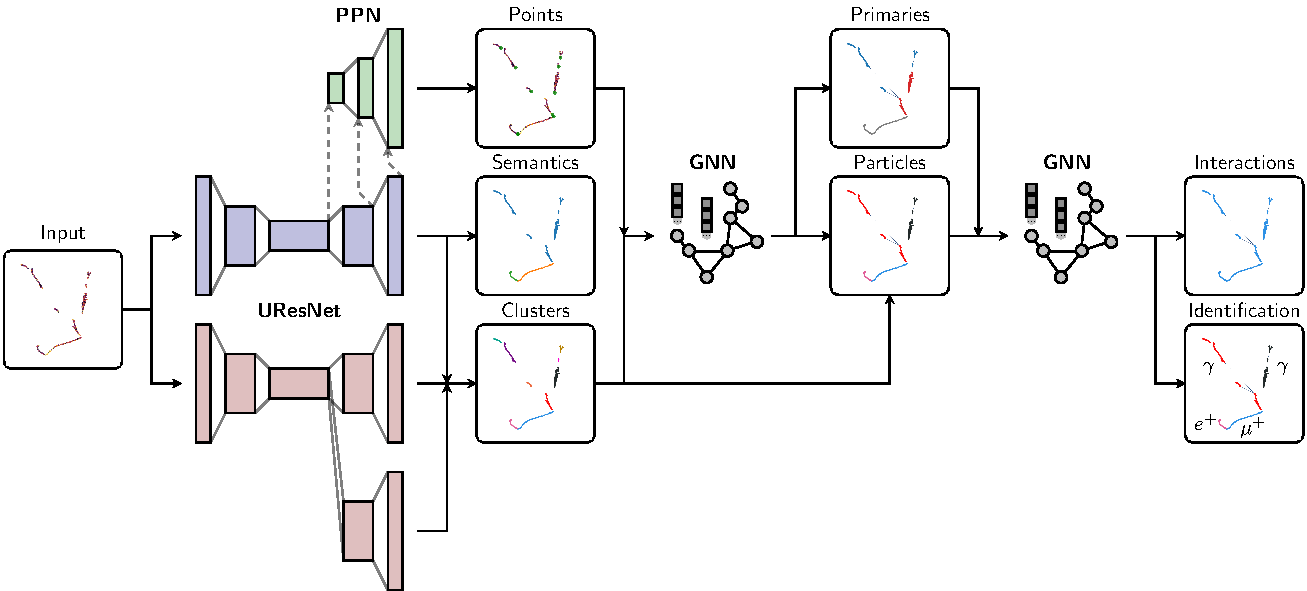
\includegraphics[width=\linewidth]{detector/mlreco_full_chain.pdf}
    \caption[SPINE end-to-end machine learning approach]{Schematic architecture of the end-to-end, ML-based reconstruction chain for LArTPCs. Picture taken from \cite{Drielsma:2021jdv}. }
    \label{fig:SPINE}
\end{figure}

The next step in the reconstruction chain is the classification of the deghosted 3D hits into categories based on the activity that produced them --- tracks, electromagnetic showers, Michel electrons, delta rays and low-energy depositions. This algorithm (shown in blue in \autoref{fig:SPINE}) uses the same UResNet architecture as the previous step. In parallel with this (shown in red in \autoref{fig:SPINE}) is a similar algorithm that aims at identifying and building dense particle clusters. The two outputs are aggregated and then passed as input to the next steps of the reconstruction. 


At this point of the SPINE reconstruction chain, groups of spacepoints corresponding to particle fragments have been identified, with semantic labels assigned to them. Then, a Graph Neural Network (GNN) aims at clustering these groups of hits into particles. Two functionally identical GNNs are employed, called GrapPA-Track and GrapPA-Shower, targeting specific interaction topologies, namely tracks and showers. Details on the implementation and working principle of these algorithms are given in \cite{Drielsma:2021jdv}. 

The final stage of the SPINE reconstruction is to cluster particles into interactions. A given interaction (equivalent to a Pandora slice) is a collection of particles originating from the same interaction vertex. Particles directly associated with the interaction vertex are called primary particles, whereas other particles are labelled as secondaries. In addition to the interaction clustering, the network is also tasked with predicting the particle type (photon, electron, muon, proton, or pion; see \cite{DeepLearnPhysics:2020hut}). The architecture is still that of a GNN. The output of this network is represented by all the interaction primary particles, each with a list of secondary particles, all with their types. 

\section{Simulation of the full detector}

\begin{figure}
    \centering
    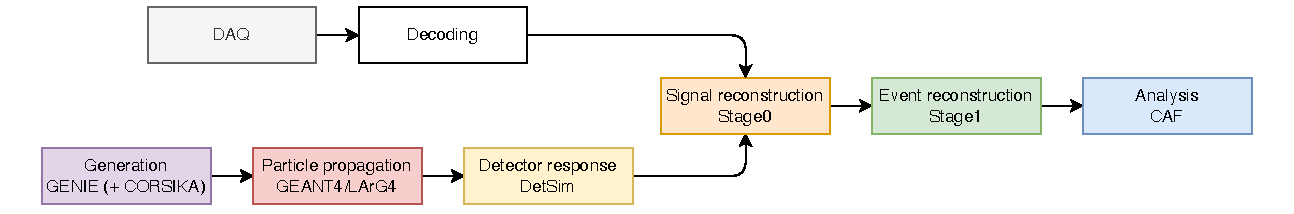
\includegraphics[width=\linewidth]{pandora/LArSoft_all.drawio.pdf}
    \caption[LArSoft complete overview]{Complete processing flow for both data and simulation, from the collection/simulation to the final analysis. }
    \label{fig:LArSoft_flow}
\end{figure}

The LArSoft framework that runs the full event reconstruction is also used to perform event simulation, from the generation of the interaction, performed using the GENIE Monte Carlo neutrino generator \cite{Andreopoulos:2015wxa}, to  particle propagation inside the LAr volume, performed using the GEANT4 package, accessed through the LArG4 framework, to detector simulation, covering all the individual subsystems of the ICARUS detector. The output of the simulation is identical to the real acquired data collected by the detector and therefore can be used to perform Monte Carlo studies on the reconstruction pipeline. Details of the full event simulation are in \cite{arteroponsStudyReconstructionNuMuCC}, and \autoref{fig:LArSoft_flow} shows a full overview of the entire pipeline both for real data, starting from the DAQ (above), to decoding and then signal processing and event reconstruction, as well as for simulated data (below).
% % !TEX root=../main.tex

\chapter{Validating the automatic Pandora-based reconstruction}\label{chap:methods}

% \dictum[M. Sotgia]{Bello studiare, ma anche la pizza}

\section{Data sample and selection}

\section{}
% % !TEX root=../main.tex

\chapter{Conclusions and future outlook}\label{chap:conclusions}

\dictum[Anonymous]{I conclude that when I'm done with my thesis, life will be better}

% \backmatter
\appendix

\chapter{Acronyms}
\stepcounter{page}

Throughout the thesis, multiple acronyms or concepts are presented and used; here are the most common with some context

\begin{abbreviations}
    BNB & Booster Neutrino Beam, the main beam feeding the SBN experiment \\
    BSM & Beyond Standard Model \\
    CC/NC & Charge/neutral current interactions \\
    CKM & Cabibbo-Kobayashi-Maskawa matrix of quark mixing \\
    CNGS & Cern Neutrinos to Gran Sasso beam \\
    Coh. & Coherent neutrino scattering \\
    DaR/DiF & Decay-at-Rest/-in-Flight \\
    DIS & Deep inelastic scattering interaction \\
    DUNE & Deep Underground Neutrino Experiment \\
    ES & Elastic scattering interaction \\
    GALLEX \newline GALLEX+GNO & Gallium neutrino observatory at LNGS \\
    ICARUS \newline \emph{or SBN-FD} & \emph{Imaging Cosmic And Rare Underground Signals}, as it was called in the Gran Sasso era, now Far Detector in the SBN experiment \\
    LArTPC & Liquid Argon Time Projection Chamber \\
    LSND & Liquid Scintillator Neutrino Detector \\
    LEP & Large Electron Positron collider \\
    LNGS & Laboratori Nazionali del Gran Sasso \\
    Mini(Micro)BooNE & Mini(micro) Booster Neutrino Experiment \\ 
    MSW & Mikheyev-Smirnov-Wolfenstein oscillation of neutrinos in matter effect \\ 
    NO/NH \newline \emph{and} IO/IH & Normal and inverted ordering/hierarchy of neutrino masses \\
    NOvA & NuMI Off-axis $\PGne$ Appearance \\
    NuMI & Neutrinos at the Main Injector \\
    PMNS & Pontecorvo-Maki-Nakagawa-Sakata matrix of neutrino oscillation \\
    PMT & Photomultiplier tubes \\
    QE & Quasielastic interactions \\
    Res. & Resonant pion production interaction \\
    SAGE & Soviet-American Gallium experiment \\
    SBN & The Short Baseline Neutrino experiment, consisting of the three detectors on the BNB baseline \\
    SBND & Short Baseline neutrino Near Detector \\ 
    SK & Super Kamiokande \\ 
    SM & the Standard Model of particle physics \\
    SNO & Sudbury Neutrino Observatory \\
    S$\Pp\PAp$S & Super Proton (anti)Proton Synchrotron \\ 
\end{abbreviations}


% % !TEX root=../main.tex

\chapter{Cheating the track/shower MVA module}

Pandora developers already provide a valid module that cheat the true information for the track/shower classification stage. This fills the PFO metadata with the correct pdg, i.e. assigns pdg $= \pm 13$ \emph{iff} the particle is \PGmpm; 

For the analysis performed in this work the 

\lstinputlisting[style=xmlstyle, language=XML]{7_listings/PandoraSettings_Neutrino_cMva.xml}


\bibliographystyle{5_bsts/utphys}
% \bibliography{4_references/references, 4_references/bibsets, 4_references/Theses}
\bibliography{thesis/4_references/EXPERIMENTAL/experimentalICARUS,thesis/4_references/THEORY/theoryNeutrinos, thesis/4_references/THEORY/theorySterile, thesis/4_references/THEORY/theoryThesis} 

\end{document}
